%  LaTeX support: latex@mdpi.com 
%  For support, please attach all files needed for compiling as well as the log file, and specify your operating system, LaTeX version, and LaTeX editor.

%=================================================================
\documentclass[futureinternet,review,accept,pdftex,moreauthors]{Definitions/mdpi} 
% For posting an early version of this manuscript as a preprint, you may use "preprints" as the journal and change "submit" to "accept". The document class line would be, e.g., \documentclass[preprints,article,accept,moreauthors,pdftex]{mdpi}. This is especially recommended for submission to arXiv, where line numbers should be removed before posting. For preprints.org, the editorial staff will make this change immediately prior to posting.
\usepackage{ wasysym }
\usepackage{ amssymb }
%%%%Update on 23 December 2021%%%
\usepackage[normalem]{ulem} % For using the command \uuline{} in the \abstract 
\usepackage{amsfonts} % Use for some special math mark
%%\usepackage{pxfonts} % Use for some special math mark 
\usepackage{wasysym} % Use for some special mark
%\usepackage{subfigure} % For some paper the use \subfigure
\usepackage{mathcomp} % For permille mark
\usepackage{CJKutf8} % For Chinese font
\usepackage{pifont} % For some special mark 
\usepackage{bm} % Forr math enviroment bold format
\graphicspath{{./Definitions/}} % Use for import path the figures paper used

% For advanced cross-references for floats for XML2PDF
\usepackage{cleveref}
\crefname{figure}{Figure}{Figures}
\crefname{table}{Table}{Tables}
\crefrangelabelformat{figure}{#3#1#4--#5#2#6}
\crefrangelabelformat{table}{#3#1#4--#5#2#6}
\crefname{section}{Section}{Sections}
\crefname{paragraph}{Section}{Sections}
\crefrangelabelformat{section}{#3#1#4--#5#2#6}
\crefname{appendix}{Appendix}{Appendices}
\crefrangelabelformat{appendix}{#3#1#4--#5#2#6}
\crefname{scheme}{Scheme}{Schemes}
\crefrangelabelformat{scheme}{#3#1#4--#5#2#6}
\crefname{chart}{Chart}{Charts}
\crefrangelabelformat{chart}{#3#1#4--#5#2#6}
\newcommand{\fig}[1]{Figure~\ref{#1}}
\newcommand{\sect}[1]{Section~\ref{#1}}
\newcommand{\tabref}[1]{Table~\ref{#1}}
\newcommand{\sche}[1]{Scheme~\ref{#1}}
\newcommand{\equ}[1]{\ref{#1}}
\newcommand{\boxref}[1]{Box~\ref{#1}}
\newcommand{\app}[1]{Appendix~\ref{#1}}
\newcommand{\cchart}[1]{Chart~\ref{#1}}

% I don't what the below codes are for?
\makeatletter
\def\T@n@@nc@d@ngM@cr@M@d{}
\def\LY@n@@nc@d@ngM@cr@M@d{}
\makeatother

\let\orignewcommand\newcommand  % Store the original \newcommand
\let\newcommand\providecommand  % Make \newcommand behave like \providecommand
\usepackage{verse}
\let\newcommand\orignewcommand  % Use the original `\newcommand` in future
\makeatletter
\renewcommand*{\theHpoemline}{\arabic{verse@envctr}.\arabic{poemline}} % Use the original definition from verse.sty
\makeatother

% Define a matrix envrioment
\newsavebox\foobox
\newcommand{\slantbox}[2][.2]{\mbox{%
        \sbox{\foobox}{#2}%
        \hskip\wd\foobox
        \pdfsave
        \pdfsetmatrix{1 0 #1 1}%
        \llap{\usebox{\foobox}}%
        \pdfrestore
}}

%\setlength{\fboxsep}{0cm}

% Define triangledown mark
\let\oldblacktriangledown\blacktriangledown

% Define \dagger using unicode
\renewcommand{\dagger}{\mathchar"2279}
\renewcommand{\ddagger}{\mathchar"227A}

% Define italic In, Max
\newcommand{\mmathit}[1]{
  \ifthenelse{\equal{#1}{\ln}}{\mathit{ln}}{
    \ifthenelse{\equal{#1}{\max}}{\mathit{max}}{\mathit{#1}}
  }
}
\makeatother
\robustify{\footnote} % I don't know what it is for? Maybe for Chicago journal footnote?

\pdfstringdefDisableCommands{% % I don't know what it is for?
\def\footnote#1{}%
}


\DeclareUnicodeCharacter{1E45}{\.{n}}
\DeclareUnicodeCharacter{1E41}{\.{m}}
\DeclareUnicodeCharacter{2003}{\quad}
%\DeclareUnicodeCharacter{0177}{\^{y}}
%\DeclareUnicodeCharacter{101}{\={a}}
\DeclareUnicodeCharacter{2009}{\thinspace}
\DeclareUnicodeCharacter{2002}{\enspace{}}
\DeclareUnicodeCharacter{2005}{\thinspace}
\DeclareUnicodeCharacter{0263}{\textipa{G}}
%\DeclareUnicodeCharacter{117}{\.{e}}
\DeclareUnicodeCharacter{A0}{~}
\DeclareUnicodeCharacter{2460}{\textcircled{\scriptsize{1}}}
\DeclareUnicodeCharacter{2461}{\textcircled{\scriptsize{2}}}
\DeclareUnicodeCharacter{2462}{\textcircled{\scriptsize{3}}}
\DeclareUnicodeCharacter{2463}{\textcircled{\scriptsize{4}}}
\DeclareUnicodeCharacter{2464}{\textcircled{\scriptsize{5}}}
\DeclareUnicodeCharacter{2465}{\textcircled{\scriptsize{6}}}
\DeclareUnicodeCharacter{2466}{\textcircled{\scriptsize{7}}}
\DeclareUnicodeCharacter{2467}{\textcircled{\scriptsize{8}}}
\DeclareUnicodeCharacter{2468}{\textcircled{\scriptsize{9}}}
\DeclareUnicodeCharacter{2070}{\textsuperscript{0}}
\DeclareUnicodeCharacter{2074}{\textsuperscript{4}}
\DeclareUnicodeCharacter{2075}{\textsuperscript{5}}
\DeclareUnicodeCharacter{2076}{\textsuperscript{6}}
\DeclareUnicodeCharacter{2077}{\textsuperscript{7}}
\DeclareUnicodeCharacter{2078}{\textsuperscript{8}}
\DeclareUnicodeCharacter{2079}{\textsuperscript{9}}
\DeclareUnicodeCharacter{02C2}{<}
\DeclareUnicodeCharacter{2033}{''}
\DeclareUnicodeCharacter{0229}{\c{e}}
\DeclareUnicodeCharacter{016F}{\r{u}}
%\DeclareUnicodeCharacter{0218}{\cb{S}}
%\DeclareUnicodeCharacter{0219}{\cb{s}}
%\DeclareUnicodeCharacter{021B}{\cb{t}}
\DeclareUnicodeCharacter{3AC}{\relax\ifmmode\acute{\alpha}\else $\acute{\alpha}$\fi}
\DeclareUnicodeCharacter{3AD}{\relax\ifmmode\acute{\varepsilon}\else $\acute{\varepsilon}$\fi}
\DeclareUnicodeCharacter{3AE}{\relax\ifmmode\acute{\eta}\else $\acute{\eta}$\fi}
\DeclareUnicodeCharacter{3AF}{\relax\ifmmode\acute{\iota}\else $\acute{\iota}$\fi}
\DeclareUnicodeCharacter{3CC}{\relax\ifmmode\acute{o}\else $\acute{o}$\fi}
\DeclareUnicodeCharacter{3CD}{\relax\ifmmode\acute{\upsilon}\else $\acute{\upsilon}$\fi}
\DeclareUnicodeCharacter{3CE}{\relax\ifmmode\acute{\omega}\else $\acute{\omega}$\fi}
\DeclareUnicodeCharacter{391}{A}
\DeclareUnicodeCharacter{392}{B}
\DeclareUnicodeCharacter{395}{E}
\DeclareUnicodeCharacter{396}{Z}
\DeclareUnicodeCharacter{397}{H}
\DeclareUnicodeCharacter{399}{I}
\DeclareUnicodeCharacter{39A}{K}
\DeclareUnicodeCharacter{39C}{M}
\DeclareUnicodeCharacter{39D}{N}
\DeclareUnicodeCharacter{39F}{O}
\DeclareUnicodeCharacter{3A1}{P}
\DeclareUnicodeCharacter{3A4}{T}
\DeclareUnicodeCharacter{3A7}{X}

\DeclareUnicodeCharacter{27E6}{\relax\ifmmode \llbracket \else $\llbracket$\fi}
\DeclareUnicodeCharacter{27E7}{\relax\ifmmode \rrbracket \else $\rrbracket$\fi}

\DeclareUnicodeCharacter{1D434}{\relax\ifmmode A \else $A$\fi}
\DeclareUnicodeCharacter{1D435}{\relax\ifmmode B \else $B$\fi}
\DeclareUnicodeCharacter{1D436}{\relax\ifmmode C \else $C$\fi}
\DeclareUnicodeCharacter{1D437}{\relax\ifmmode D \else $D$\fi}
\DeclareUnicodeCharacter{1D438}{\relax\ifmmode E \else $E$\fi}
\DeclareUnicodeCharacter{1D439}{\relax\ifmmode F \else $F$\fi}
\DeclareUnicodeCharacter{1D43A}{\relax\ifmmode G \else $G$\fi}
\DeclareUnicodeCharacter{1D43B}{\relax\ifmmode H \else $H$\fi}
\DeclareUnicodeCharacter{1D43C}{\relax\ifmmode I \else $I$\fi}
\DeclareUnicodeCharacter{1D43D}{\relax\ifmmode J \else $J$\fi}
\DeclareUnicodeCharacter{1D43E}{\relax\ifmmode K \else $K$\fi}
\DeclareUnicodeCharacter{1D43F}{\relax\ifmmode L \else $L$\fi}
\DeclareUnicodeCharacter{1D440}{\relax\ifmmode M \else $M$\fi}
\DeclareUnicodeCharacter{1D441}{\relax\ifmmode N \else $N$\fi}
\DeclareUnicodeCharacter{1D442}{\relax\ifmmode O \else $O$\fi}
\DeclareUnicodeCharacter{1D443}{\relax\ifmmode P \else $P$\fi}
\DeclareUnicodeCharacter{1D444}{\relax\ifmmode Q \else $Q$\fi}
\DeclareUnicodeCharacter{1D445}{\relax\ifmmode R \else $R$\fi}
\DeclareUnicodeCharacter{1D446}{\relax\ifmmode S \else $S$\fi}
\DeclareUnicodeCharacter{1D447}{\relax\ifmmode T \else $T$\fi}
\DeclareUnicodeCharacter{1D448}{\relax\ifmmode U \else $U$\fi}
\DeclareUnicodeCharacter{1D449}{\relax\ifmmode V \else $V$\fi}
\DeclareUnicodeCharacter{1D44A}{\relax\ifmmode W \else $W$\fi}
\DeclareUnicodeCharacter{1D44B}{\relax\ifmmode X \else $X$\fi}
\DeclareUnicodeCharacter{1D44C}{\relax\ifmmode Y \else $Y$\fi}
\DeclareUnicodeCharacter{1D44D}{\relax\ifmmode Z \else $Z$\fi}
\DeclareUnicodeCharacter{1D44E}{\relax\ifmmode a \else $a$\fi}
\DeclareUnicodeCharacter{1D44F}{\relax\ifmmode b \else $b$\fi}
\DeclareUnicodeCharacter{1D450}{\relax\ifmmode c \else $c$\fi}
\DeclareUnicodeCharacter{1D451}{\relax\ifmmode d \else $d$\fi}
\DeclareUnicodeCharacter{1D452}{\relax\ifmmode e \else $e$\fi}
\DeclareUnicodeCharacter{1D453}{\relax\ifmmode f \else $f$\fi}
\DeclareUnicodeCharacter{1D454}{\relax\ifmmode g \else $g$\fi}
\DeclareUnicodeCharacter{1D456}{\relax\ifmmode i \else $i$\fi}
\DeclareUnicodeCharacter{1D457}{\relax\ifmmode j \else $j$\fi}
\DeclareUnicodeCharacter{1D458}{\relax\ifmmode k \else $k$\fi}
\DeclareUnicodeCharacter{1D459}{\relax\ifmmode l \else $l$\fi}
\DeclareUnicodeCharacter{1D45A}{\relax\ifmmode m \else $m$\fi}
\DeclareUnicodeCharacter{1D45B}{\relax\ifmmode n \else $n$\fi}
\DeclareUnicodeCharacter{1D45C}{\relax\ifmmode o \else $o$\fi}
\DeclareUnicodeCharacter{1D45D}{\relax\ifmmode p \else $p$\fi}
\DeclareUnicodeCharacter{1D45E}{\relax\ifmmode q \else $q$\fi}
\DeclareUnicodeCharacter{1D45F}{\relax\ifmmode r \else $r$\fi}
\DeclareUnicodeCharacter{1D460}{\relax\ifmmode s \else $s$\fi}
\DeclareUnicodeCharacter{1D461}{\relax\ifmmode t \else $t$\fi}
\DeclareUnicodeCharacter{1D462}{\relax\ifmmode u \else $u$\fi}
\DeclareUnicodeCharacter{1D463}{\relax\ifmmode v \else $v$\fi}
\DeclareUnicodeCharacter{1D464}{\relax\ifmmode w \else $w$\fi}
\DeclareUnicodeCharacter{1D465}{\relax\ifmmode x \else $x$\fi}
\DeclareUnicodeCharacter{1D466}{\relax\ifmmode y \else $y$\fi}
\DeclareUnicodeCharacter{1D467}{\relax\ifmmode z \else $z$\fi}

\DeclareUnicodeCharacter{1E67}{\.{\v s}}
\DeclareUnicodeCharacter{1E11}{\relax\ifmmode \c{d} \else $\c{d}$\fi}
\DeclareUnicodeCharacter{1ECB}{\relax\ifmmode \d{i} \else $\d{i}$\fi}
\DeclareUnicodeCharacter{1D8D}{\relax\ifmmode \textlhookx \else $\textlhookx$\fi}
\DeclareUnicodeCharacter{104}{\relax\ifmmode \k{A} \else $\k{A}$\fi}
\DeclareUnicodeCharacter{211E}{\relax\ifmmode \textrecipe \else $\textrecipe$\fi}
\DeclareUnicodeCharacter{29D}{\relax\ifmmode \textctj \else $\textctj$\fi}

\DeclareUnicodeCharacter{1E2E}{\'{\"I}}
\DeclareUnicodeCharacter{23F}{\textrts}

\DeclareUnicodeCharacter{2C73}{\varw}

\DeclareUnicodeCharacter{2127}{\mho}

\DeclareUnicodeCharacter{28C}{\textturnv}
\DeclareUnicodeCharacter{252}{\textturnscripta}
\DeclareUnicodeCharacter{259}{\schwa}
\DeclareUnicodeCharacter{25B}{\m{e}}
\DeclareUnicodeCharacter{266}{\m{h}}
\DeclareUnicodeCharacter{127}{\B{h}}
\DeclareUnicodeCharacter{27E}{\textfishhookr}
\DeclareUnicodeCharacter{281}{\textinvscr}


\usepackage{hyperref}
%\makeatletter
%\g@addto@macro{\UrlBreaks}{\UrlOrds}
%\makeatother
\makeatletter
\def\UrlAlphabet{%
\do\a\do\b\do\c\do\d\do\e\do\f\do\g\do\h\do\i\do\j%
\do\k\do\l\do\m\do\n\do\o\do\p\do\q\do\r\do\s\do\t%
\do\u\do\v\do\w\do\x\do\y\do\z\do\A\do\B\do\C\do\D%
\do\E\do\F\do\G\do\H\do\I\do\J\do\K\do\L\do\M\do\N%
\do\O\do\P\do\Q\do\R\do\S\do\T\do\U\do\V\do\W\do\X%
\do\Y\do\Z}
\def\UrlDigits{\do\1\do\2\do\3\do\4\do\5\do\6\do\7\do\8\do\9\do\0}
\g@addto@macro{\UrlBreaks}{\UrlOrds}
\g@addto@macro{\UrlBreaks}{\UrlAlphabet}
\g@addto@macro{\UrlBreaks}{\UrlDigits}
\makeatother

%--------------------
% Class Options:
%--------------------
%----------
% journal
%----------
% Choose between the following MDPI journals:
% acoustics, actuators, addictions, admsci, adolescents, aerospace, agriculture, agriengineering, agronomy, ai, algorithms, allergies, alloys, analytica, animals, antibiotics, antibodies, antioxidants, applbiosci, appliedchem, appliedmath, applmech, applmicrobiol, applnano, applsci, aquacj, architecture, arts, asc, asi, astronomy, atmosphere, atoms, audiolres, automation, axioms, bacteria, batteries, bdcc, behavsci, beverages, biochem, bioengineering, biologics, biology, biomass, biomechanics, biomed, biomedicines, biomedinformatics, biomimetics, biomolecules, biophysica, biosensors, biotech, birds, bloods, blsf, brainsci, breath, buildings, businesses, cancers, carbon, cardiogenetics, catalysts, cells, ceramics, challenges, chemengineering, chemistry, chemosensors, chemproc, children, chips, cimb, civileng, cleantechnol, climate, clinpract, clockssleep, cmd, coasts, coatings, colloids, colorants, commodities, compounds, computation, computers, condensedmatter, conservation, constrmater, cosmetics, covid, crops, cryptography, crystals, csmf, ctn, curroncol, currophthalmol, cyber, dairy, data, dentistry, dermato, dermatopathology, designs, diabetology, diagnostics, dietetics, digital, disabilities, diseases, diversity, dna, drones, dynamics, earth, ebj, ecologies, econometrics, economies, education, ejihpe, electricity, electrochem, electronicmat, electronics, encyclopedia, endocrines, energies, eng, engproc, ent, entomology, entropy, environments, environsciproc, epidemiologia, epigenomes, est, fermentation, fibers, fintech, fire, fishes, fluids, foods, forecasting, forensicsci, forests, foundations, fractalfract, fuels, futureinternet, futureparasites, futurepharmacol, futurephys, futuretransp, galaxies, games, gases, gastroent, gastrointestdisord, gels, genealogy, genes, geographies, geohazards, geomatics, geosciences, geotechnics, geriatrics, hazardousmatters, healthcare, hearts, hemato, heritage, highthroughput, histories, horticulturae, humanities, humans, hydrobiology, hydrogen, hydrology, hygiene, idr, ijerph, ijfs, ijgi, ijms, ijns, ijtm, ijtpp, immuno, informatics, information, infrastructures, inorganics, insects, instruments, inventions, iot, j, jal, jcdd, jcm, jcp, jcs, jdb, jeta, jfb, jfmk, jimaging, jintelligence, jlpea, jmmp, jmp, jmse, jne, jnt, jof, joitmc, jor, journalmedia, jox, jpm, jrfm, jsan, jtaer, jzbg, kidney, kidneydial, knowledge, land, languages, laws, life, liquids, literature, livers, logics, logistics, lubricants, lymphatics, machines, macromol, magnetism, magnetochemistry, make, marinedrugs, materials, materproc, mathematics, mca, measurements, medicina, medicines, medsci, membranes, merits, metabolites, metals, meteorology, methane, metrology, micro, microarrays, microbiolres, micromachines, microorganisms, microplastics, minerals, mining, modelling, molbank, molecules, mps, msf, mti, muscles, nanoenergyadv, nanomanufacturing, nanomaterials, ncrna, network, neuroglia, neurolint, neurosci, nitrogen, notspecified, nri, nursrep, nutraceuticals, nutrients, obesities, oceans, ohbm, onco, oncopathology, optics, oral, organics, organoids, osteology, oxygen, parasites, parasitologia, particles, pathogens, pathophysiology, pediatrrep, pharmaceuticals, pharmaceutics, pharmacoepidemiology, pharmacy, philosophies, photochem, photonics, phycology, physchem, physics, physiologia, plants, plasma, pollutants, polymers, polysaccharides, poultry, powders, preprints, proceedings, processes, prosthesis, proteomes, psf, psych, psychiatryint, psychoactives, publications, quantumrep, quaternary, qubs, radiation, reactions, recycling, regeneration, religions, remotesensing, reports, reprodmed, resources, rheumato, risks, robotics, ruminants, safety, sci, scipharm, seeds, sensors, separations, sexes, signals, sinusitis, skins, smartcities, sna, societies, socsci, software, soilsystems, solar, solids, sports, standards, stats, stresses, surfaces, surgeries, suschem, sustainability, symmetry, synbio, systems, taxonomy, technologies, telecom, test, textiles, thalassrep, thermo, tomography, tourismhosp, toxics, toxins, transplantology, transportation, traumacare, traumas, tropicalmed, universe, urbansci, uro, vaccines, vehicles, venereology, vetsci, vibration, viruses, vision, waste, water, wem, wevj, wind, women, world, youth, zoonoticdis 
  \graphicspath{ {figures/}} 

%---------
% article
%---------
% The default type of manuscript is "article", but can be replaced by: 
% abstract, addendum, article, book, bookreview, briefreport, casereport, comment, commentary, communication, conferenceproceedings, correction, conferencereport, entry, expressionofconcern, extendedabstract, datadescriptor, editorial, essay, erratum, hypothesis, interestingimage, obituary, opinion, projectreport, reply, retraction, review, perspective, protocol, shortnote, studyprotocol, systematicreview, supfile, technicalnote, viewpoint, guidelines, registeredreport, tutorial
% supfile = supplementary materials

%----------
% submit
%----------
% The class option "submit" will be changed to "accept" by the Editorial Office when the paper is accepted. This will only make changes to the frontpage (e.g., the logo of the journal will get visible), the headings, and the copyright information. Also, line numbering will be removed. Journal info and pagination for accepted papers will also be assigned by the Editorial Office.

%------------------
% moreauthors
%------------------
% If there is only one author the class option oneauthor should be used. Otherwise use the class option moreauthors.

%---------
% pdftex
%---------
% The option pdftex is for use with pdfLaTeX. If eps figures are used, remove the option pdftex and use LaTeX and dvi2pdf.

%=================================================================
% MDPI internal commands
\firstpage{1} 
\makeatletter 
\setcounter{page}{\@firstpage} 
\makeatother
\pubvolume{14}
\issuenum{2}
\articlenumber{59}
\pubyear{2022}
\copyrightyear{2022}
\externaleditor{Academic Editor: {Eirini Eleni Tsiropoulou}} % pls add it.
\datereceived{21 January 2022 } 
\dateaccepted{3 February 2022} 
\datepublished{15 February 2022} 
%\externaleditor{Academic Editor: Firstname Lastname} % For journal Automation, please change Academic Editor to "Communicated by"
%\datecorrected{} % Corrected papers include a "Corrected: XXX" date in the original paper.
%\dateretracted{} % Corrected papers include a "Retracted: XXX" date in the original paper.
\hreflink{https://doi.org/10.3390/\linebreak fi14020059} % If needed use \linebreak
%\doinum{}
%------------------------------------------------------------------
% The following line should be uncommented if the LaTeX file is uploaded to arXiv.org
%\pdfoutput=1

%=================================================================
% Add packages and commands here. The following packages are loaded in our class file: fontenc, inputenc, calc, indentfirst, fancyhdr, graphicx, epstopdf, lastpage, ifthen, lineno, float, amsmath, setspace, enumitem, mathpazo, booktabs, titlesec, etoolbox, tabto, xcolor, soul, multirow, microtype, tikz, totcount, changepage, attrib, upgreek, cleveref, amsthm, hyphenat, natbib, hyperref, footmisc, url, geometry, newfloat, caption

%=================================================================
%% Please use the following mathematics environments: Theorem, Lemma, Corollary, Proposition, Characterization, Property, Problem, Example, ExamplesandDefinitions, Hypothesis, Remark, Definition, Notation, Assumption
%% For proofs, please use the proof environment (the amsthm package is loaded by the MDPI class).

%=================================================================
% Full title of the paper (Capitalized)
\Title{{Network} %article title is different from susy, please confirm.
Function Virtualization and Service Function Chaining Frameworks: A Comprehensive Review of Requirements, Objectives, Implementations, and Open Research Challenges}

% MDPI internal command: Title for citation in the left column
\TitleCitation{Network Function Virtualization and Service Function Chaining Frameworks: A Comprehensive Review of Requirements, Objectives, Implementations, and Open Research Challenges}

% Author Orchid ID: enter ID or remove command
\newcommand{\orcidauthorA}{0000-0001-5944-8473} % Add \orcidA{} behind the author's name
\newcommand{\orcidauthorB}{0000-0003-0939-378X} % Add \orcidB{} behind the author's name

% Authors, for the paper (add full first names)
\Author{Haruna Umar Adoga~*\orcidA{} and Dimitrios P. Pezaros \orcidB{} }

%\longauthorlist{yes}

% MDPI internal command: Authors, for metadata in PDF
\AuthorNames{Haruna Umar Adoga , Dimitrios P. Pezaros}

% MDPI internal command: Authors, for citation in the left column
\AuthorCitation{Adoga, H.U.; Pezaros, D.P.}
% If this is a Chicago style journal: Lastname, Firstname, Firstname Lastname, and Firstname Lastname.

% Affiliations / Addresses (Add [1] after \address if there is only one affiliation.)
\address[1]{%
School of Computing Science, University of Glasgow, Glasgow G12 8QQ, UK; dimitrios.pezaros@glasgow.ac.uk\\
}

% Contact information of the corresponding author
\corres{\hangafter=1 \hangindent=1em \hspace{-1em} Correspondence: h.adoga.1@research.gla.ac.uk}



% Abstract (Do not insert blank lines, i.e., \\) 
\abstract{Network slicing has become a fundamental property for next-generation networks, especially because an inherent part of 5G standardisation is the ability for service providers to migrate some or all of their network services to a virtual network infrastructure, thereby reducing both capital and operational costs. With network function virtualisation (NFV), network functions (NFs) such as firewalls, traffic load balancers, content filters, and intrusion detection systems (IDS) are either instantiated on virtual machines (VMs) or lightweight containers, often chained together to create a service function chain (SFC).
In this work, we review the state-of-the-art NFV and SFC implementation frameworks and present a taxonomy of the current proposals. Our taxonomy comprises three major categories based on the primary objectives of each of the surveyed frameworks: (1)~resource allocation and service orchestration, (2) performance tuning, and (3) resilience and fault recovery. We also identify some key open research challenges that require further exploration by the research community to achieve scalable, resilient, and high-performance NFV/SFC deployments in next-generation networks.}

% Keywords
\keyword{network function virtualization; service function chaining; software defined networking; next-generation networks; SFC frameworks} 

% The fields PACS, MSC, and JEL may be left empty or commented out if not applicable
%\PACS{J0101}
%\MSC{}
%\JEL{}

%%%%%%%%%%%%%%%%%%%%%%%%%%%%%%%%%%%%%%%%%%
% Only for the journal Diversity
%\LSID{\url{http://}}

%%%%%%%%%%%%%%%%%%%%%%%%%%%%%%%%%%%%%%%%%%
% Only for the journal Applied Sciences:
%\featuredapplication{Authors are encouraged to provide a concise description of the specific application or a potential application of the work. This section is not mandatory.}
%%%%%%%%%%%%%%%%%%%%%%%%%%%%%%%%%%%%%%%%%%

%%%%%%%%%%%%%%%%%%%%%%%%%%%%%%%%%%%%%%%%%%
% Only for the journal Data:
%\dataset{DOI number or link to the deposited data set in cases where the data set is published or set to be published separately. If the data set is submitted and will be published as a supplement to this paper in the journal Data, this field will be filled by the editors of the journal. In this case, please make sure to submit the data set as a supplement when entering your manuscript into our manuscript editorial system.}

%\datasetlicense{license under which the data set is made available (CC0, CC-BY, CC-BY-SA, CC-BY-NC, etc.)}

%%%%%%%%%%%%%%%%%%%%%%%%%%%%%%%%%%%%%%%%%%
% Only for the journal Toxins
%\keycontribution{The breakthroughs or highlights of the manuscript. Authors can write one or two sentences to describe the most important part of the paper.}

%%%%%%%%%%%%%%%%%%%%%%%%%%%%%%%%%%%%%%%%%%
% Only for the journal Encyclopedia
%\encyclopediadef{Instead of the abstract}
%\entrylink{The Link to this entry published on the encyclopedia platform.}
%%%%%%%%%%%%%%%%%%%%%%%%%%%%%%%%%%%%%%%%%%
\begin{document}
%%%%%%%%%%%%%%%%%%%%%%%%%%%%%%%%%%%%%%%%%%
%\setcounter{section}{-1} %% Remove this when starting to work on the template.
%\endnote{This is an endnote.} % To use endnotes, please un-comment \printendnotes below (before References). Only journal Laws uses \footnote.

% The order of the section titles is: Introduction, Materials and Methods, Results, Discussion, Conclusions for these journals: aerospace,algorithms,antibodies,antioxidants,atmosphere,axioms,biomedicines,carbon,crystals,designs,diagnostics,environments,fermentation,fluids,forests,fractalfract,informatics,information,inventions,jfmk,jrfm,lubricants,neonatalscreening,neuroglia,particles,pharmaceutics,polymers,processes,technologies,viruses,vision


\section{Introduction}
\label{sec:introduction}
With the advent of software-defined networking (SDN) and network function virtualization (NFV), middlebox functionality is increasingly being virtualized and provided in software, which can reduce power consumption, resource usage, and operational costs for service providers~\cite{herrera2016resource, cherrared2019survey}. This paradigm is a departure from the use of hardware middleboxes, which are often proprietary,  and thus not easily extendable by service providers. By abstracting network functionalities and implementing them in software, network operators can create network functions that suit their service level agreement (SLA) and service models~\cite{paganelli2021tenant}. 

NFV helps network operators by providing the right environment for the rapid deployment and scaling of virtual network functions (vNFs)~\cite{laghrissi2018survey},  which are chained together in what is known as the service function chaining (SFC) architecture. Unlike the typical routing technique employed by middleboxes, where packets are simply forwarded directly from source to destination, SFC routes packets through a chain of network functions before reaching the destination (depending on the type of service and policy in use). Thus, one of the major goals of SFC is the flexibility it offers by allowing traffic to traverse diverse network functions along the service chain. 

Heterogeneous network services deployed using SFC and virtual functions are installed on multiple virtual machines, sometimes combined with containers~\cite{bujari2019service, santos2020towards}, which are chained together to provide services to users. SFC is generally considered as one of the important use cases of NFV and SDN architectures~\cite{li2016survey}, which is also made possible using a centralised network controller that has a \textit{global} logical view of the entire network infrastructure, and handles tasks such as the creation of service chains and orchestration of traffic between vNFs~\cite{haleplidis2014forces}. In terms of the location of network functions in a service chain, the virtualized infrastructure can span multiple datacentres, which calls for inter-data-centre networking or within the same data centre, which results in an intra-data-centre network (see Section \ref{SFC-environments}).

We generally expect the SFCs to be adaptive and dynamic; service chains should have the feature of readjusting to the unpredictable nature of service requests, and to offer better quality of service (QoS) for the end user~\cite{liu2017dynamic, chua2016stringer}. If we consider network security as an example, such a service may consist of network functions such as firewalls, deep packet inspection (DPI), intrusion prevention or detection modules installed as software, which are chained together~\cite{bhamare2017optimal}.

Several implementation frameworks have been proposed in the literature, some of which have been adopted and deployed at a commercial scale, while others are in the experimental state of development. In this paper, we put together these frameworks while highlighting their contributions and how they solve research problems associated with realising NFV/SFC in service provider network environments. 

Experts from both academia and industry are putting a lot of effort in the research and development of SFC. While NFV/SFC has developed over the years, developments in this domain are so substantial that it makes a survey now quite different and valuable from a (hypothetical) survey put together a few years ago. Unlike previous surveys in this area, our work (layout in Figure \ref{Paper-Structure}) also shows how SDN, NFV, and SFC are combined in the provisioning, operations, and management of next-generation networks. We further explain how our work differs from previous efforts by presenting related surveys in Section~\ref{MOTIVATION}; thus, our contributions are threefold:

%%%%%%%%%%%%%%%%%%%%%%%%
\begin{figure}[H]%[H]
%\centering
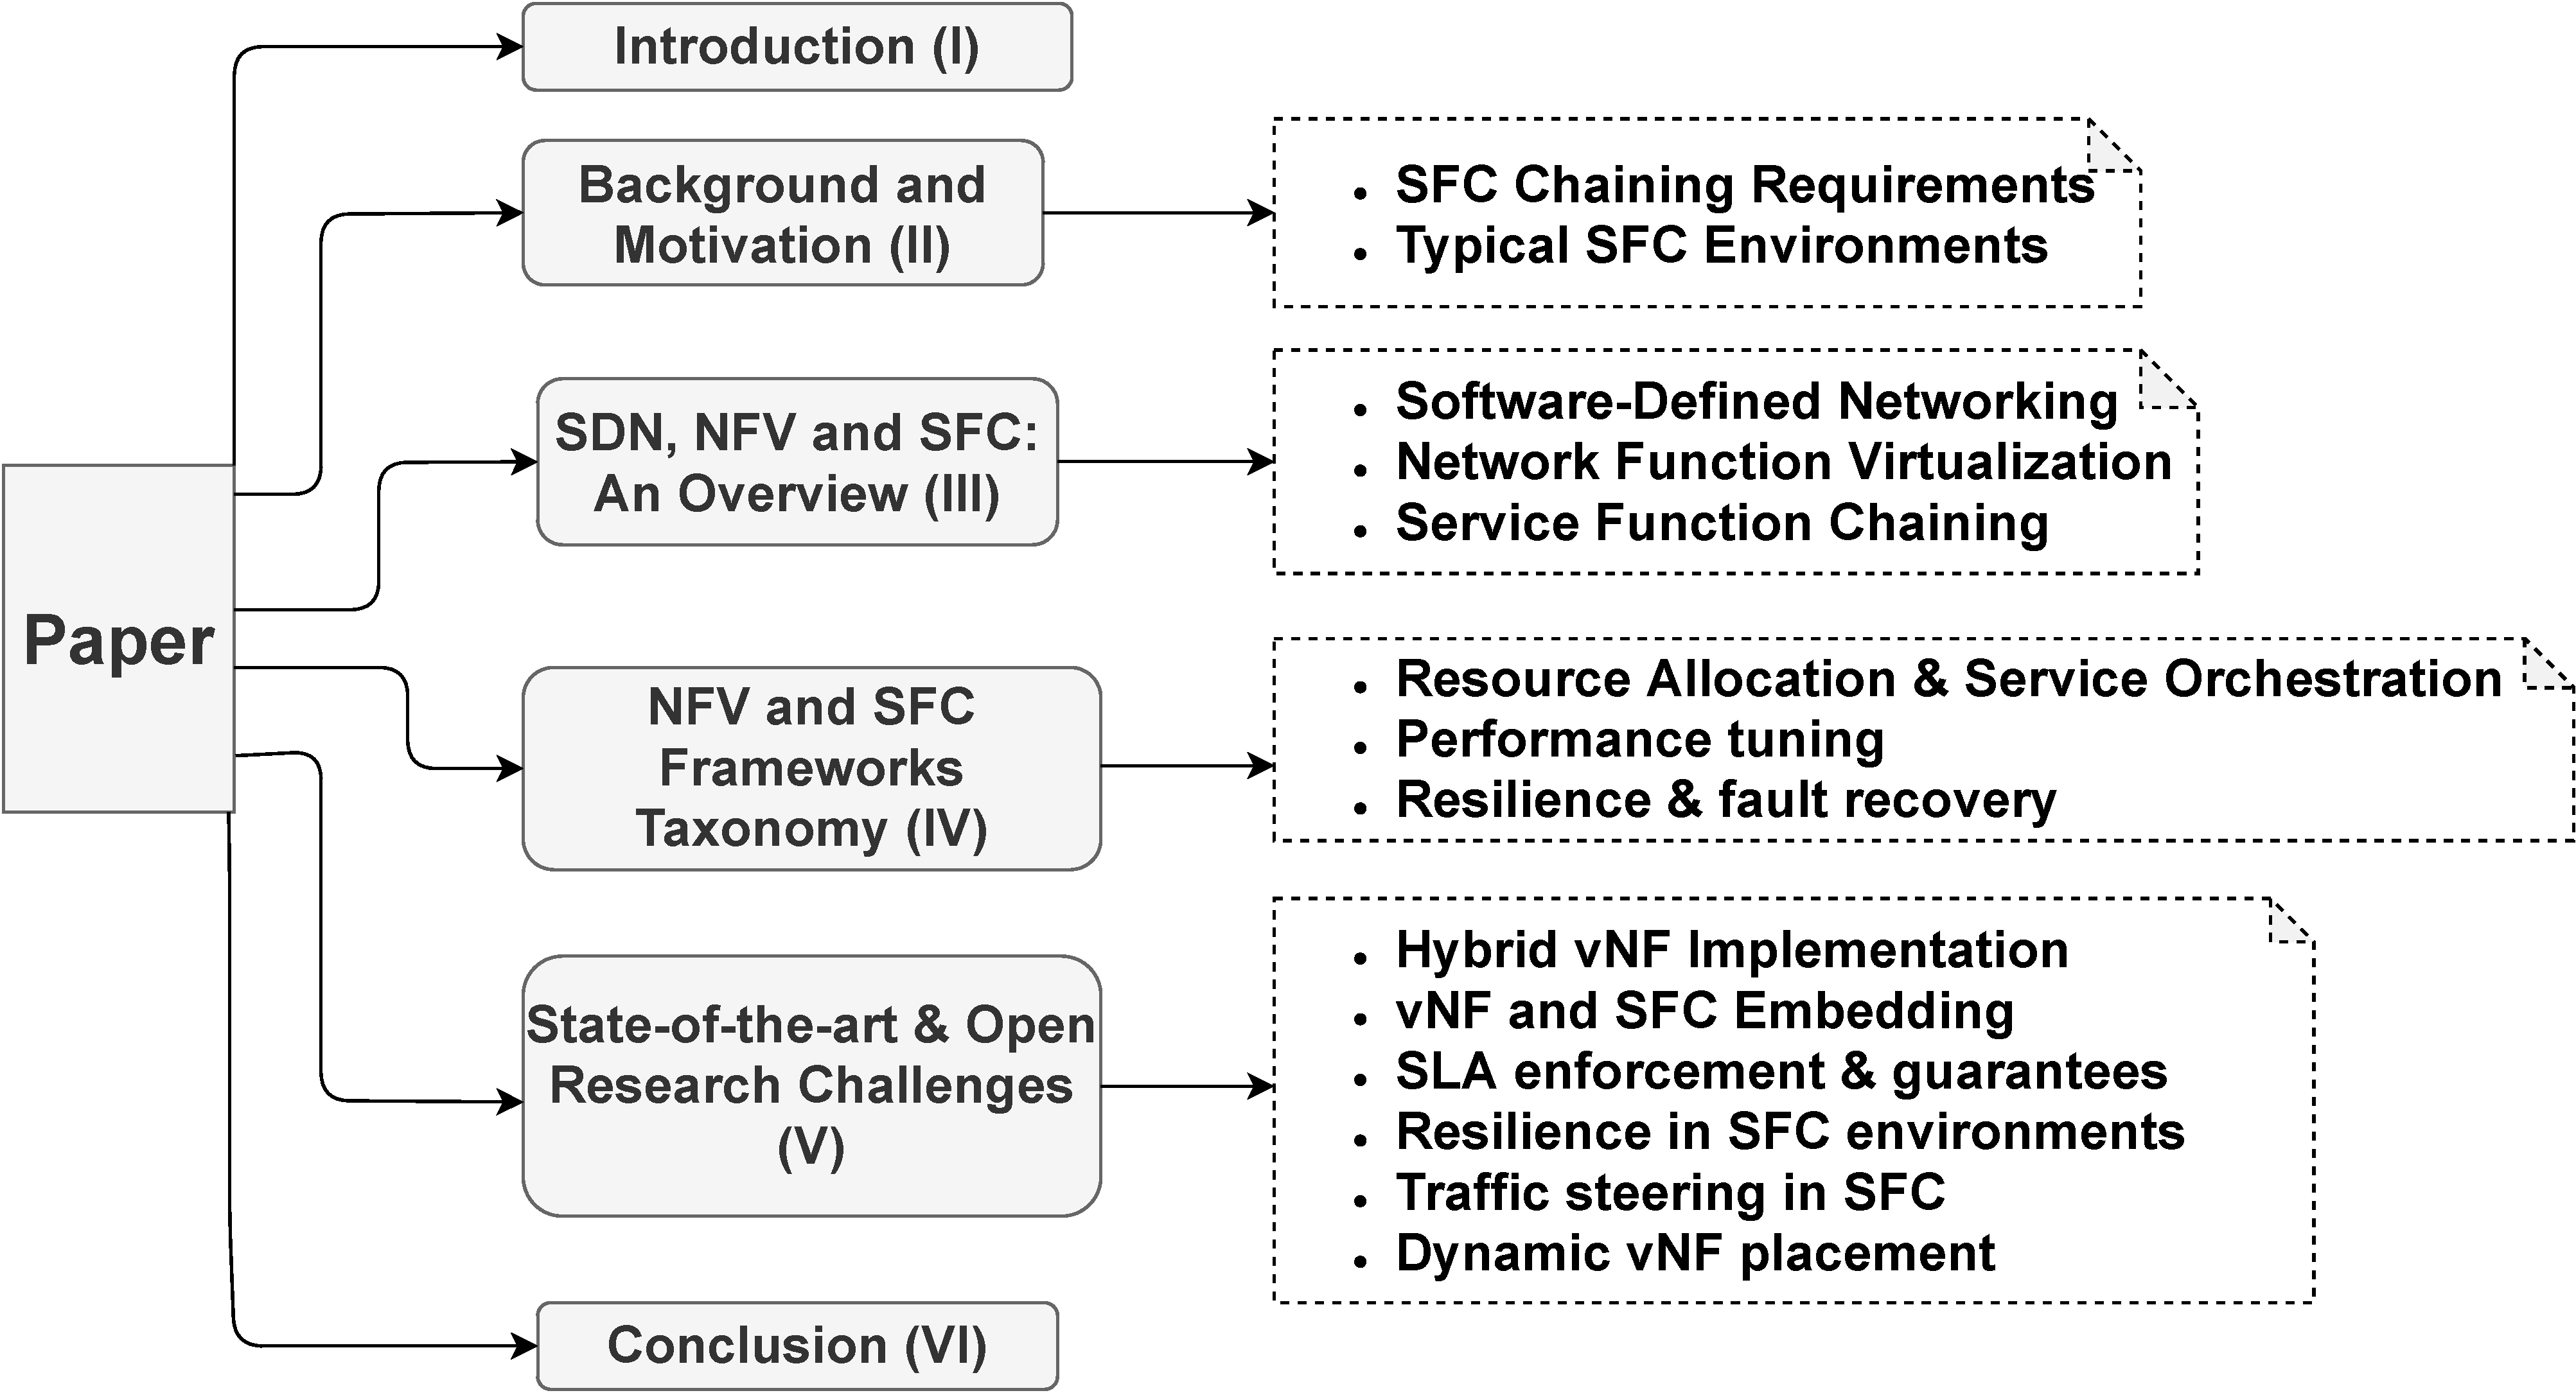
\includegraphics[width=0.9\columnwidth]{Paper_Structure.pdf}
\caption{High-level paper structure.}
\label{Paper-Structure}
\end{figure}
%%%%%%%%%%%%%%%%%%%%%%
%contributions!
\begin{itemize}
    \item We present the vNF chaining requirements (Section \ref{SFC-requirements}) and how they relate to SFC implementations in service provider networks, thus some use cases for the SFC paradigm (Section \ref{SFC-environments}) are presented. An overview of the current state-of-the-art SDN, NFV, and SFC (Section \ref{SDN-NFV-SFC}) is also presented as the foundation for the frameworks reviewed in this paper;
    
    \item We present a comprehensive survey of the state-of-the-art NFV frameworks for building and implementing vNFs, particularly frameworks that have been proposed for use in SFC environments. We also present a taxonomy of SFC implementation frameworks,  focusing on each SFC-related challenge, each one addressing the approaches used (Section \ref{SFC implementation frameworks}); %please verify
    
    \item Finally, we identify and discuss the main open research challenges associated with NFV and SFC environments in the next generation networks (Section \ref{Open-challenges}). 
\end{itemize} 

The remainder of this paper is structured as follows: Section \ref{MOTIVATION} presents the background and motivation of this survey, considering what has been done in the literature and  highlighting the uniqueness of our approach and reflections on the state of the art approaches. %please verify
Section 
\ref{SDN-NFV-SFC} briefly discusses the underlying technological advancements that make NFV possible. Section
\ref{SFC implementation frameworks} contains a taxonomy of the implementation frameworks considered in this work, classifying the frameworks into three major categories. The problems addressed by the frameworks are presented in {Table} 3 (resource allocation and service orchestration),  {Table} 4 (performance tunning) and {Table} 5 (resilience and fault recovery)  which represent various aspects of the SFC implementation challenges. We present the state-of-the-art SFC and highlight the open research challenges of NFV/SFC environments in Section \ref{Open-challenges}. Finally, Section \ref{Conclusion} concludes the paper.



\subsection*{Research Methodology}
\label{methodology}
Our work covers research performed in recent years in the area of NFV/SFC implementation frameworks. The methodology employed involved a critical review of the relevant contributions in report papers, journals, conference papers, and articles. We systematically queried the most relevant scholarly databases (IEEE, ACM Digital library, Web of Science, Scopus, etc.) to get all the required research papers that are relevant to our work. We started this process with 367 papers, of which 118 papers met our final selection criteria. 

We made use of some basic exclusion criteria (Figure \ref{Data_Extraction-pic}) such as the exclusion of papers that were written in languages other than English, papers with no full text, research papers in duplicates, the year of publication, and the specific area(s) covered such as focusing on research papers in areas related to NFV, SFC, and SDN in service provider network~environments. 

%%%%%%%%%%%%%%%%%%%%%%%%
\begin{figure}[H]%[H]
%\centering
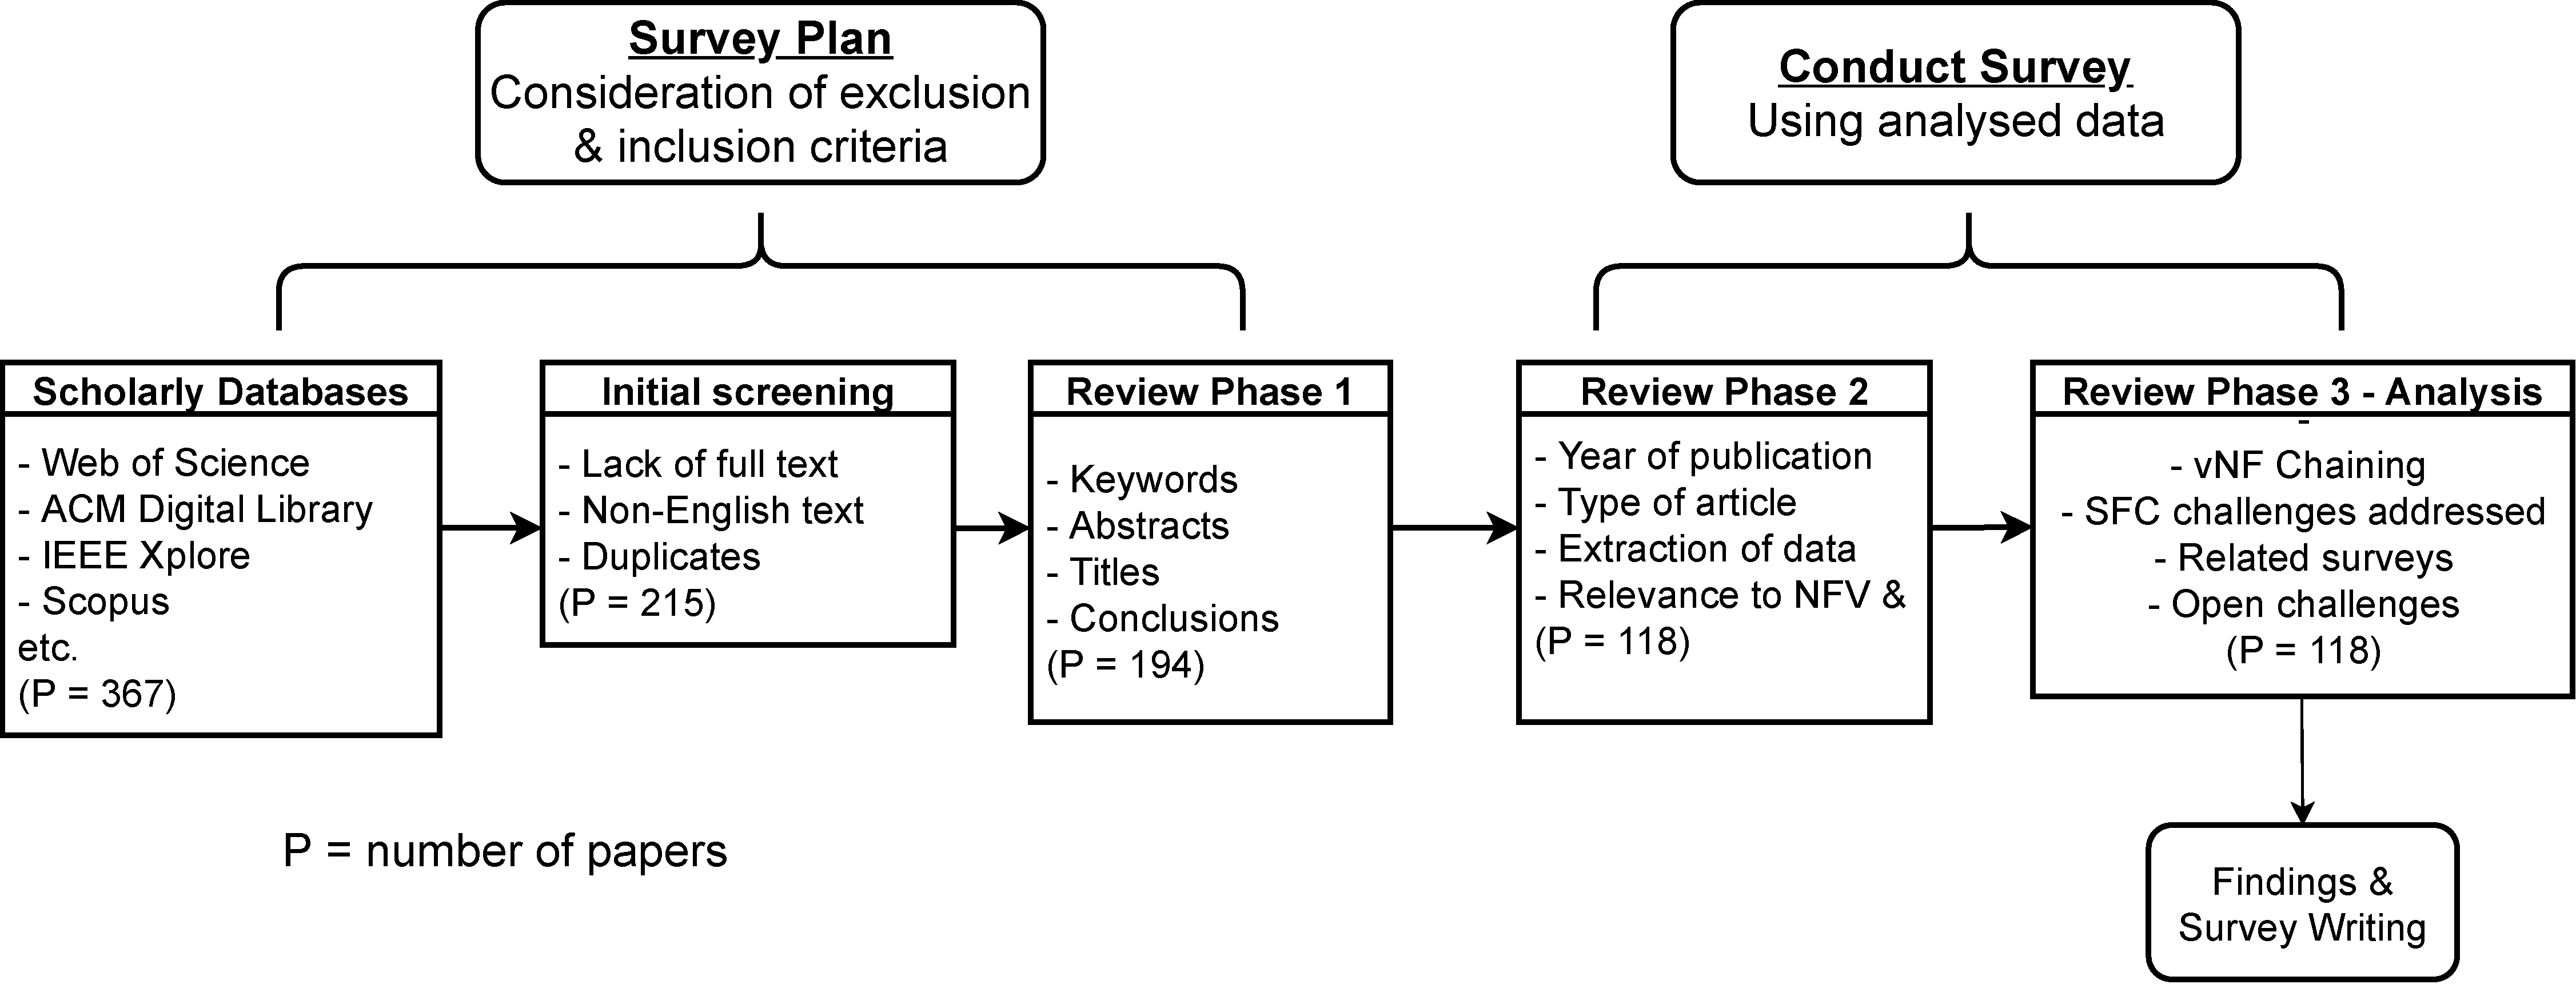
\includegraphics[width=.95\columnwidth]{Data_Extraction.pdf}
\caption{Paper analysis process.}
\label{Data_Extraction-pic}
\end{figure}
%%%%%%%%%%%%%%%%%%%%%%

For the review of papers presented in our proposed taxonomy, we included research papers that present NFV implementation frameworks with some vNF chaining components, representative frameworks that address specific problems in the domain, e.g., vNF orchestration, traffic steering, SFC resilience, modular SFC deployment, etc. A total of 118~papers were finally selected, which include some notable related surveys, and experimental and theoretical works in NFV/SFC. The papers we have cited in our taxonomy cover fundamental equivalence classes of the state-of-the-art in NFV/SFC implementation~frameworks. 

In addition to the more recent research papers presented in our work, we would like to note that some of the papers we considered present both the pioneering efforts for certain equivalence classes of NFV/SFC frameworks and still represent the state-of-the-art; thus, the most recent works (if any) are incremental to what we have presented. As a concrete example that justifies some of our choices (based on current literature), frameworks such as ClickOS~\cite{martins2014clickos}, OpenNetVM~\cite{zhang2016opennetvm}, OpenBox~\cite{bremler2016openbox}, Slick~\cite{anwer2015programming}, SNF~\cite{katsikas2016snf}, Metron~\cite{katsikas2018metron}, NetBricks~\cite{panda2016netbricks}, and GNF~\cite{cziva2015container} constitute some of the notable pioneering efforts in this domain, which are still relevant in designing NFV/SFC frameworks for next generation~networks.

Each of these frameworks represent important aspects such as the use of lightweight packet processing elements, the use of packet acceleration frameworks, the decoupling of network infrastructure into control and data-planes, synthesizing packet processing elements for improved performance, resource allocation, and deploying containerized network functions at the network edge to support the edge computing paradigm. In terms of technological advancements and existing works in the literature, we have covered the core components that are still used in designing and implementing NFV/SFC frameworks to the best of our knowledge.  
%%%%%%%%%%%%%%%%%%%%%%%%%%%%%%%%%%%%%%%%%%

%%%%%%%%%%%%%%%%%%%%%%%%%%%%%%%%%%%%%
%%%%%%%%%%%%%%%%%%%%%%%%%%%%%%%%%%%%%
\section{Background and Motivation} 
\label{MOTIVATION}
There are several existing studies that focus on the general areas of SDN, NFV, and SFC, as summarised in Table \ref{Related Survey}. Each of the related surveys presented in our work explores different aspects such as NFV implementation problems, traffic steering in SFC, NFV deployment acceleration, optimal NFV and SFC concepts, design, and taxonomy of NFV platforms, the placement of network functions, and resource allocation. This section summarises the key contributions made by existing related surveys and provides the foundation for our research.

%%%%%%%%%%%%%%%%%%%%%%%%%%%%%%%%%
%\newpage
\begin{table}[H]
%%\centering
\caption{Existing NFV/SFC Surveys.}
\label{Related Survey}
\tablesize{\footnotesize}
% \resizebox{\textwidth}{!}{%
	\begin{adjustwidth}{-\extralength}{0cm}
		\setlength{\cellWidtha}{\fulllength/4-2\tabcolsep-0.3in}
\setlength{\cellWidthb}{\fulllength/4-2\tabcolsep+1.6in}
\setlength{\cellWidthc}{\fulllength/4-2\tabcolsep-0.1in}
\setlength{\cellWidthd}{\fulllength/4-2\tabcolsep-1.2in}
\scalebox{1}[1]{\begin{tabularx}{\fulllength}{>{\PreserveBackslash\centering}m{\cellWidtha}>{\PreserveBackslash\centering}m{\cellWidthb}>{\PreserveBackslash\centering}m{\cellWidthc}>{\PreserveBackslash\centering}m{\cellWidthd}}

\toprule


\textbf{Survey Reference} & \multicolumn{1}{c}{\textbf{Survey Focus}}&\textbf{Open Challenges Presented} & \textbf{Year} \\ \midrule 

Zoure {et al.}~\cite{zoure2022network} & Network services anomalies in NFV & \ding{52} & 2022 \\ %\hline

Zhang {et al.}~\cite{zhang2020nfv} & NFV platforms, design and taxonomy & \ding{52} & 2021 \\ %\hline

Hamdan {et al.}~\cite{hamdan2021comprehensive} & Load balancing techniques in SDN & \ding{52} & 2021 \\ %\hline
Fei {et al.}~\cite{fei2020paving} & NFV deployment acceleration & \ding{52} & 2020 \\%\hline

Kaur {et al.}~\cite{kaur2020comprehensive} & vNF placement, availability, and load balancing & \ding{52} & 2020\\ %\hline

Hantouti {et al.}~\cite{hantouti2020service} & Service function, 5G and next-generation networks & \ding{52} & 2020 \\ %\hline

Bonfim {et al.}~\cite{bonfim2019integrated} & NFV architectures; NFV/SDN design taxonomy & \ding{52} & 2019 \\ %\hline

Hantouti {et al.}~\cite{hantouti2018traffic} & Traffic steering in SFC; SDN-based chaining evaluation & \ding{52} & 2019\\ %\hline

Laghrissi {et al.}~\cite{laghrissi2018survey} & Service placement survey; vNF placement; existing virtual resource placement solutions & Lessons learned & 2019 \\ %\hline

Mirjalily {et al.}~\cite{mirjalily2018optimal} & Optimal NFV and SFC concepts & \ding{52} & 2018\\ %\hline

Medhat {et al.}~\cite{medhat2016service} & Next Generation Network SFC; SDN approaches in SFC; SFC implementations & Implementation limitations & 2017 \\ %\hline


Bera {et al.}~\cite{bera2017software} & SDN for IoT & \ding{52} & 2017\\ %\hline
Veeraraghavan {et al.}~\cite{veeraraghavan2017network} & NFV survey; selected implementation problems and solutions & \ding{56} & 2017\\ %\hline

Bhamare {et al.}~\cite{bhamare2016survey} & Service function chaining; NFV mobility & \ding{52} & 2016\\ %\hline

Herrera {et al.} ~\cite{herrera2016resource} & NFV resource allocation & \ding{52} & 2016\\ %\hline 

Xie {et al.}~\cite{xie2016service} & Resource allocation in SFC; Existing NFV SFC RA solutions & Lessons learned & 2016\\ 
%\hline

Li {et al.}~\cite{li2016survey} & Network function placement; Selected framework comparison &\ding{52} & 2016\\ %\hline

Yang {et al.}~\cite{yang2015software} & SDN/NFV for mobile and wireless networks & \ding{52} & 2015\\
	\bottomrule
		\end{tabularx}}
	\end{adjustwidth}
\end{table}
%%%%%%%%%%%%%%%%%%%%%%%
\vspace{-6pt}

As one of the most recent survey works in the NFV/SFC space, Fei {et al.}~\cite{fei2020paving} focused their work on the proposals that consider the acceleration of NFV deployments. A taxonomy of the surveyed approaches is presented and discussed, which mainly involves the hardware and software acceleration of NFV deployments. We take a different approach by considering the state-of-the-art NFV implementation frameworks, especially in scenarios where network functions are also chained, as in SFCs.

In their work, Zhang {et al.}~\cite{zhang2020nfv} presented NFV platform design choices. They presented three main open issues in NFV: (1) the use of artificial intelligence in NFV, (2) network slicing, that is, the management of network slices, the communication between slices and placement of network slices, and (3) the integration of NFV with IoT. The taxonomy of NFV platforms presented by Zhang {et al.} consists of prototyping, testing, deployment, management, execution, and integrated NFV platforms. We take a different approach in our work by first presenting the requirements that must be met for the chaining of vNFs and some useful use-cases. This is relevant in understanding the key components involved in creating service function chains in service provider network environments. Our work focuses mainly on NFV frameworks that employ the chaining of network functions for effective service delivery. In addition to the taxonomy of the frameworks presented, we also discuss key open research challenges in these environments.

In the survey presented by Hantouti {et al.}~\cite{hantouti2018traffic}, they discussed the traffic steering approaches used in SFC solutions with SDN. The current traffic steering approaches are classified into three methods: header-based, tag-based, and programmable switch-based methods. They concluded by identifying QoS, scalability, security, and management as some of the challenges in SFC traffic steering. Although their survey is comprehensive in terms of SDN-based traffic steering in SFC, we focus our work not only on traffic steering in SFC, but also on the implementation frameworks used to achieve a scalable, resilient, and high-performance SFC.

Bonfim {et al.}~\cite{bonfim2019integrated} presented a review of integrated NFV/SDN architectures, where they considered implementation frameworks that combined NFV and SDN. They identified vNF scheduling and placement, improving network programmability, and the possibility of deploying multiple SDN controllers to achieve scalability, security, and standardisation of SDN/NFV solutions as some of the open challenges. We extend their contributions by considering proposals that implement NFV/SFC and the challenges that require \mbox{further~research.}

As one of the early attempts in this domain, the survey by Yang {et al.}~\cite{yang2015software} explores the challenges faced in mobile and wireless network (MWN) environments. Their work carefully describes how software-defined wireless networks (SDWNs) and wireless network virtualization (WNV) can be used in addressing the challenges of MWN networks.

A survey on SFC was presented by Herrera {et al.}~\cite{herrera2016resource} and Xie {et al.}~\cite{xie2016service}, where the authors focused on resource allocation approaches in the literature. Medhat {et al.}~\cite{medhat2016service} presented open challenges in service function chaining for next-generation networks. A taxonomy of prior work was presented, where they classified it into data -and control-plane SFC solutions. Our survey considers a broader scope by creating a taxonomy that is beyond control and data-plane solutions, as well as presenting state-of-the-art technologies and open research challenges.

Bhamare {et al.}~\cite{bhamare2016survey} presented a detailed survey of SFC, where the authors identified optimal resource allocation, dynamic service mapping, and policy enforcement, as some of the challenges in these environments. Li {et al.}~\cite{li2016survey} and Laghrissi {et al.}~\cite{laghrissi2018survey} focused on the placement of resources in SFC environments, where the former presented a survey of network function placement in SFC, and the latter focused on the placement of virtual resources. In their survey, Hamdan {et al.}~\cite{hamdan2021comprehensive} explored the traffic load balancing approaches used in SDN network environments. Our work presents the relationship between SDN, NFV, and SFC, as well as a novel taxonomy of implementation frameworks.

Mirjalily {et al.}~\cite{mirjalily2018optimal} presented a survey of SFC and NFV implementation efforts. Some of the future research directions presented by~\cite{mirjalily2018optimal} include SLA and QoS approaches, online chaining of service functions, availability and resilience of chains, security, and energy efficiency. Our survey provides a more technical look into the implementation frameworks by first classifying the state-of-the-art frameworks and the proposed solutions.

The comprehensive survey presented by Bera {et al.}~\cite{bera2017software} focus on SDN technologies employed in network environments such as the data centre, edge, access, and core networks. They present their findings in relation to IoT use cases. They identified open research challenges such as platform independence, policy enforcement, mobility management, and the fully practical implementations of SDN-based solutions in IoT environments. 

In their comprehensive survey, Kaur {et al.}~\cite{kaur2020comprehensive} classified SDN/NFV approaches into availability, placement, and load-balancing solutions. They identified the ordering of SFCs, resiliency, security, topology configuration, and service placement, as some of the challenges related to current SFC implementations. We extend this work by (1) creating a taxonomy that captures state-of-the-art frameworks; (2) presenting frameworks that also capture the chaining of vNFs, which is key to the design of next-generation networks ; and (3) presenting more open challenges that are key to achieving scalability of network functions, resilience, and high performance in NFV/SFC network environments.

 
The survey carried out by Hantouti {et al.}~\cite{hantouti2020service} on SFC challenges covered frameworks that proposed to solve challenges such as path selection, orchestration, security, SFC path composition, QoS, and traffic steering. They concluded by acknowledging that more work needs to be done in developing related technologies (SDN and NFV). We also consider frameworks that focus on areas such as resilience, fault recovery, performance tuning, and resource allocation to extend their contributions.

%Addressing reviewer's concern
To the best of our knowledge, we have summarised the key contributions of notable related surveys and how our work adds to the NFV/SFC domain. Unlike most existing surveys, our research also presents the detailed requirements for chaining virtual network functions in service provider environments, including some important use cases. The taxonomy we created in our work presents the design choices and technologies used for the implementation of different equivalence classes of NFV/SFC frameworks. This focuses on the existing problems in the NFV/SFC domain, that is, we categorise the surveyed frameworks based on their proposed solutions and technological design choices.
 
 Most of the notable related surveys we have presented only discuss the technologies and open challenges in the NFV or SFC domain. Some exceptions to this are the surveys by Bonfim et al., which present a taxonomy of NFV/SDN architectures by categorising them into NFV-side and SDN-side designs, while Zhang et al. presented a taxonomy based on the life cycle of NFV platforms. Kaur et al. presented a taxonomy based on the optimisation approaches used in SFC, such as availability, placement, and load balancing. In contrast to previous surveys, we categorise the surveyed frameworks based on their proposed solutions and technological design choices. 
 
 We carefully describe what each framework has been designed to achieve, what technology and approach have been used, and what performance (or other quality) benchmarks have been performed. We have also highlighted the different methods and technologies used for  implementing each framework. In addition to presenting an extensive list of open research challenges in NFV/SFC, we also discuss some notable early  attempts in the literature aimed at addressing the research challenges identified (Section \ref{Open-challenges}), providing  the reader with knowledge of some existing efforts in this direction. 



\subsection{SFC Chaining Requirements}
\label{SFC-requirements}
When it comes to the chaining of network functions in an SFC environment, the IETF SFC draft~\cite{quinn2014service} provides an architectural framework that captures all the components that are required for SFC implementation in service provider networks.

There are some useful assumptions that need to be considered when creating a chain of network functions: (1) different network functions present their own configuration and description challenges, thus, creating a generalised description for all service functions is not trivial; (2) the implementation environment of the network function affects the list of functions that can exist in a particular domain; (3) the logic employed for the chaining of service functions is not fixed, that is, it is peculiar to any given administrative domain and the requirements of service(s) to be delivered to end users; and (4) the invocation of any service chaining criteria depends on the administrative domain in which the service functions are deployed~\cite{quinn2014service}. 


In terms of chaining requirements, although there are domain-specific requirements that need to be in place when deploying SFCs (based on the network administrative domain), there are also general requirements for the components that are found in most SFC deployments~\cite{gasparakis2016evaluating}. Irrespective of the network environment(s), {\textit{global}} %MDPI: Is the italics necessary?
 components must be in place. These components are the service classifier, which is placed at the entry point of the network (to classify ingress flows). Flow classification helps with the decision-making process of the orchestrator in terms of traffic steering across the service chain.

The service function forwarder (SFF) is another component that forwards received traffic to the right service function (SF), and can be embedded on a physical network component or deployed as a virtual component along the service function path (SFP), which is based on the classification of ingress traffic performed by the SC~\cite{halpern2015service}. The SFF is also responsible for handling any return traffic that needs to be forwarded back to a specific service function or service classifier in the service chain~\cite{quinn2014service}.

Another component is the SFC proxy, which is often optional in SFC implementations and used in scenarios where other components (SF and SFF) are unable to communicate in the chain~\cite{hantouti2020service}. SFC deployments can be fully deployed without the use of any form of proxy component, that is, when SFC-unaware service functions are not deployed in the network infrastructure. In situations where SFC-unaware service functions are part of the service chain, an SFC proxy is used to add or remove encapsulation information; thus, these are considered as {\textit{logical}} components of the SFC architecture~\cite{quinn2014service}. 
Figure \ref{SFC-Components-Figure} depicts some of the core components of the IETF SFC architecture.


%%%%%%%%%%%%%%%%%%%%%%%%
\begin{figure}[H]%[H]
%\centering
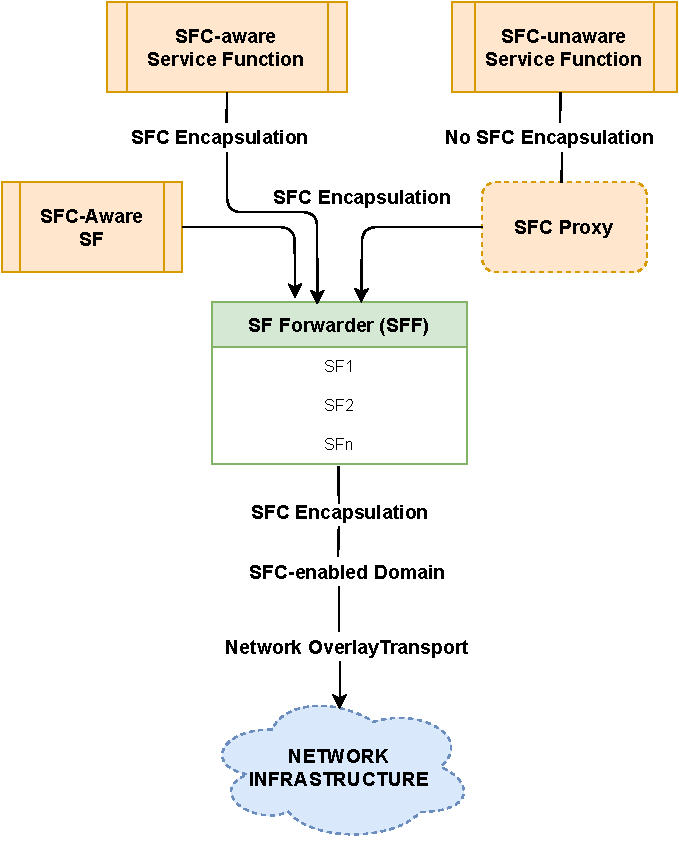
\includegraphics[width=0.5\columnwidth]{SFC-COMPONENTS.pdf}
\caption{IETF SFC Architecture Components.}
\label{SFC-Components-Figure}
\end{figure}
%%%%%%%%%%%%%%%%%%%%%%

%%%%%%%%%%%%%%%%%%%%%%%%%%%%%%%%%%%%%%%%%%%%%%%
%%%%%%%%%%%%%%%%%%%%%%%%%%%%%%%%%%%%%%%%%%%%%%%
\subsection{Typical SFC Environments}
\label{SFC-environments}
As more network operators continue to adopt network slicing, which serves as the enabler for next-generation networks, the chaining of virtual network functions for efficient service delivery has become commonplace. Some common use cases can be found in today's service provider networks. Some available common environments are the Gi-LAN network used by mobile network operators, residential/consumer services, and inter/intra-data-centre networks. Mobile network operators deploy functions such as traffic optimizers, firewalls, carrier-grade network address translation (NAT), load balancers, and DPI, at the core of the network, which is designed for subscribers that access Internet-based services~\cite{gronsund2015solution}. Here, we briefly explore these environments.

%%%%%%%%%%%%%%
\subsubsection{The Gi-LAN Mobile Core Network}
\label{Gi-LAN}
A typical environment in which service function chaining is deployed is the Gi-LAN network, which is a component of mobile networks used by operators to provide fine-grained user-specific services such as traffic optimisation, DPI, and firewalls~\cite{naik2017libvnf}. Gi-LAN implementation by mobile network operators is an emerging use case for SFC architecture~\cite{turk2019implementation}. These services are often chained together and are provided by multiple vendors, and the traffic is steered to the right service functions, which is aimed at meeting service level agreements and policy enforcement~\cite{kaurroad}.

The ability to add or remove a service becomes easier along the processing pipeline, as per-user services can be created for mobile data monetisation~\cite{brown2015service}. In terms of implementation requirements, implementing a service chain that contains a network function such as NAT, for example, requires that the function is placed on the edge sites, which is closer to the users requesting the service~\cite{shojafar2019recent}. Another useful requirement when creating a service chain in a mobile core environment is the consideration of the SLA agreement between multiple vendors. For packet classification requirements, the classifier should be located at the packet gateway. Figure \ref{Gi-LAN-Figure} depicts a high-level description of the SFC in mobile networks, with service functions deployed in the Gi-LAN segment of the network.


\begin{figure}[H]%[h]
%\centering
%\includegraphics[width=0.8\textwidth]{SDN.png}
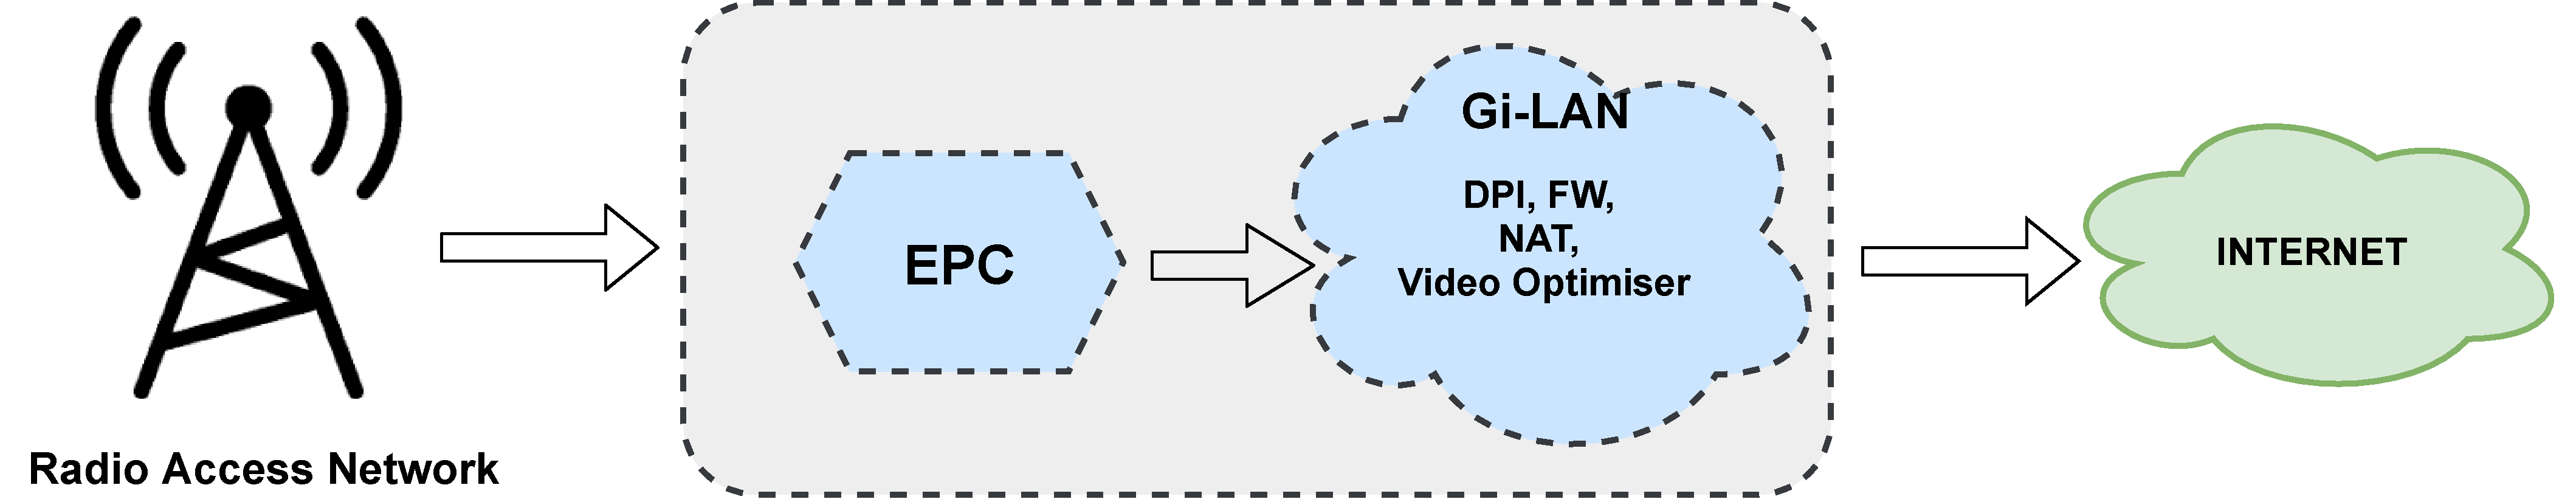
\includegraphics[width=1\columnwidth]{Gi-LAN.pdf}
\caption{Gi-LAN in mobile networks.}
\label{Gi-LAN-Figure}
\end{figure}


%%%%%%%%%%%%%
\subsubsection{Residential and Consumer Services}
Because NFV/SDN allows for the provisioning of highly specialised solutions to meet customers' quality of service requirements, using the concept of service function chaining, service providers can steer residential traffic such as parental control and VoIP-related services. The idea of follow-the-user service deployment in residential environments is an important use case that is achieved using SFC implementations.

Network operators make use of vCPEs to easily create a chain of services that meet user requirements~\cite{cunha2016policy}. Users in these environments are more likely to make use of web-based applications that use HTTP as the de facto protocol~\cite{shojafar2019recent}. One of the requirements for such deployments is to create a service chain that prioritises security~\cite{yan2016security}. A typical example is a service chain which follows the order: firewall $>$ IDS $>$ proxy. Security of users is a priority and an important requirement, especially in this scenario.

%%%%%%%%%%%%%%%%%%
\subsubsection{Inter-and Intra-Data-Centre Networks}
SFC in the inter/intra DC environment allows for the chaining of virtualized enterprise network applications (in the case of intra-data-center) and chaining across multiple locations, or inter-cloud, in the case of inter-data-centre networking. The ability of service functions to be instantiated across multiple datacenters (inter-data-centre networking) is a key requirement for live VM migration. The SFC architecture to be implemented should be designed to dynamically migrate service functions from one VM/container to another without disrupting user service requests~\cite{liu2021disaster}. 

Deploying and managing service function chains in an inter-data-center setting incurs inter-data-centre bandwidth cost, deployment cost, intra-data-centre cost, and vNF costs~\cite{zhong2018service}. In these environments, NFs are also used for policy-based routing of cloud services and enterprise applications~\cite{gronsund2015solution}, which means that service providers can up-sell their services easily using SFC at the enterprise. This can be achieved by making network services user-programmable.



%%%%%%%%%%%%%%%%%%%%%%%%%%%%%%%%%%%%%%%%%%%
%%%%%%%%%%%%%%%%%%%%%%%%%%%%%%%%%%%%%%%%%%%
\section{SDN, NFV, and SFC: An Overview} 
\label{SDN-NFV-SFC}
In service provider networks, the process of creating, deleting, modifying, and steering traffic in SFCs is carried out efficiently by using SDN and NFV technologies~\cite{medhat2016resilient}. These technologies are the key networking paradigms that are at the core of the frameworks surveyed in our study. In this section, we describe these technologies as they relate to NFV/SFC implementation frameworks in service provider network environments, thus showing their interrelation in the operations of next-generation networks. Even though the chaining of hardware middle-boxes is possible, the use of NFV makes it much easier and cheaper~\cite{sarmiento2021decentralized}. Thus, SDN is employed for orchestrating virtual network functions by providing a centralised logical control and the creation of service chains.

%%%%%%%%%%%%%%%%%%%%%%%%%%%%%%%%%%%%%%%%%
\subsection{Software-Defined Networking}
\label{SDN_Overview}
Software-defined networking decouples the control plane from the data plane in the networking devices. Traditional non-SDN networks often have control and data planes integrated on a single device, which brings about challenges such as management complexity and scalability issues. Implementing centralised network control using SDN controllers results in easier service deployment and management~\cite{sarmiento2021decentralized}. This helps service providers to easily steer traffic between NFs by scaling across multiple physical machines. 

%%%%%%%%%%%%%%%%%%%%%%%%%%%%%%%%%%%%%%%%%%%%%%%%%%%%%%%%%%%%%%%%%%%%%%%

%%%%%%%%%%%%%%%%%%%%%%%%%%%%%%%%%%%%%%%%%%%%%%%%%%%%%%%%%%%%%%%%%%%%%%
The functional separation of the network infrastructure into control and data planes, as shown in Figure \ref{SDNseparation}, is the core concept behind SDN. The application layer consists of various network applications, providing network services that use the Northbound Interfaces for sending requests to the control plane (centralised logical control). A global view of the network infrastructure is maintained by an SDN controller such as OpenDaylight~\cite{medved2014opendaylight}, POX~\cite{kaur2014network}, RYU 
{\url{https://ryu-sdn.org/}}  ({accessed} % Please add access date.
on 12 December 2021), or a custom-built controller can be used to manage network functions, which handles requests coming from the network applications, and sends instructions to the data plane of the network for packet processing~\cite{zhang2021performance}.
%%We add the footnote in the text, please confirm.
\begin{figure}[H]%[H]
%\centering
\includegraphics[width=.99\textwidth]{SDNseparation.pdf}
%\includegraphics[width=\columnwidth]{SDNseparation.png}
\caption{OpenFlow SDN and P4 data-plane.}
\label{SDNseparation}
\end{figure}
Using the southbound application programming interfaces (APIs) and the OpenFlow protocol, rules are sent down to devices in the data plane of the network, which is responsible for packet processing and forwarding. Although traditional SDN networks  use the OpenFlow protocol to communicate with the network data plane by inserting flow rules on devices, the network has become more programmable over the years. Programmability allows network operators to define the processing pipeline and how packets are processed using high-level languages such as P4~\cite{bosshart2014p4}.

Figure \ref{SDNseparation} depicts a high-level comparison of the operation of OpenFlow SDN and programmable data planes, where P4 programs are written and compiled and then deployed on programmable switches. This allows for the creation of a highly programmable pipeline, as opposed to a fixed (less flexible) processing pipeline found in OpenFlow SDN. SDN and NFV serve as the building blocks for reaching the goal of deploying a chain of virtual network functions in the service provider network environment.

%%

%%%%%%%%%%%%%%%%%%%%%%%%%%%%%%%%%%%%%%%%%%%%%%%%%

%%%%%%%%%%%%%%%%%%%%%%%%%%%%%


%%%%%%%%%%%%%%%%%%%%%%%%%%%%%%%%%%%%%%%%%%%%%%%%%%%
\subsection{Network Function Virtualization}
\label{NFV}
The use of proprietary network hardware is expensive for service providers in terms of procurement, security, configuration, scalability, and maintenance costs. The European Telecommunications Standards Institute (ETSI)~\cite{etsi2013network} introduced a high-level NFV architectural framework, envisaging the deployment of network functions as software, running on the network function virtual infrastructure (NFVI), which could be a general-purpose server. This proposal was introduced to take advantage of hardware virtualisation~\cite{binu2011virtualization,wray2012network}. The deployment of network services has been greatly simplified by NFV, because the cost of acquiring new hardware middle-boxes is reduced, and several middle boxes can be virtualized and deployed on single or multiple general-purpose servers.
%%%%%%%%%%%%%%%%%%%%%%%%%%%%

%%%%%%%%%%%%%%%%%%%%%%%%%%%%%%%%%%%%%%%%%%%%%

The ETSI architectural framework for NFV depicted in Figure \ref{NFV} shows all the important components that are necessary for deploying NFV. The operations support system (OSS) and business support system (BSS) directly interact with the vNFs. The vNF component is the network functionality, for example, a traffic load balancer, a WAN optimizer, and a firewall, etc. (Table \ref{VNF-Table}). The hardware infrastructure consists of a virtual infrastructure with virtual computing, storage, and network components. This infrastructure is managed by the virtual infrastructure manager (VIM), which is responsible for resource allocation and embedding of virtual network functions on the virtual infrastructure. NFV Orchestrator (NFVO), which is an integral part of the ETSI NFV framework~\cite{etsi2013network}, is responsible for service orchestration and management~\cite{medhat2016service}. One of the functions of the orchestration layer is the mapping of virtual network functions in a service chain to available physical resources. The management and network orchestration (MANO) component is responsible for the orchestration of vNFs and the chaining of services in a scenario where service function chaining is used. As shown in the SFC scenario in Figure \ref{Service Function Chaining}, general-purpose hardware could be a typical high-performance commercial off-the-shelf (COTS) hardware~\cite{etsi2013network}.

\begin{table}[H]
\tablesize{\small}
\caption{Commonly used vNFs in NFV.\label{VNF-Table}}
	\begin{adjustwidth}{-\extralength}{0cm}
		\newcolumntype{C}{>{\centering\arraybackslash}X}
		\begin{tabularx}{\fulllength}{CC}
			\toprule
			\textbf{vNF} & \textbf{Functionality} \\
\midrule
Application gateway & Layer 7 traffic management based on application profile \\ %\hline
Layer 2 forwarder & Packet forwarding based on layer 2 information\\ %\hline
Protocol Analyzer & Packet classification, based on protocol in use \\ %\hline
Flow tracker & Storing, displaying and forwarding ingress flows\\ %\hline
Layer 3 Switch/Router & Traffic routing and switching using IP addresses \\ %\hline
Application Firewall & Layer 3 and layer 7 packet filtering  \\ %\hline
Bridge & Bridging between two networks or host devices \\ %\hline
Carrier Grade NAT & IP address translation for WAN connectivity \\ %\hline
IDS/IPS & Stateful or stateless intrusion detection and prevention \\ %\hline
Protocol converter & Protocol translation between IPv4 to IPv6 \\ %\hline
Encryption gateway & Packet encapsulation and packet encryption/decryption\\ %\hline
ACL & User and application level access control  \\ %\hline
Protocol Accelerators & Performance improvements by ISPs \\ %\hline
VLAN manager & VLAN encapsulation and decapsulation \\
	\bottomrule
		\end{tabularx}
	\end{adjustwidth}
\end{table}
\unskip

\begin{figure}[H]%[H]
%\centering
%\includegraphics[width=0.8\textwidth]{SDN.png}
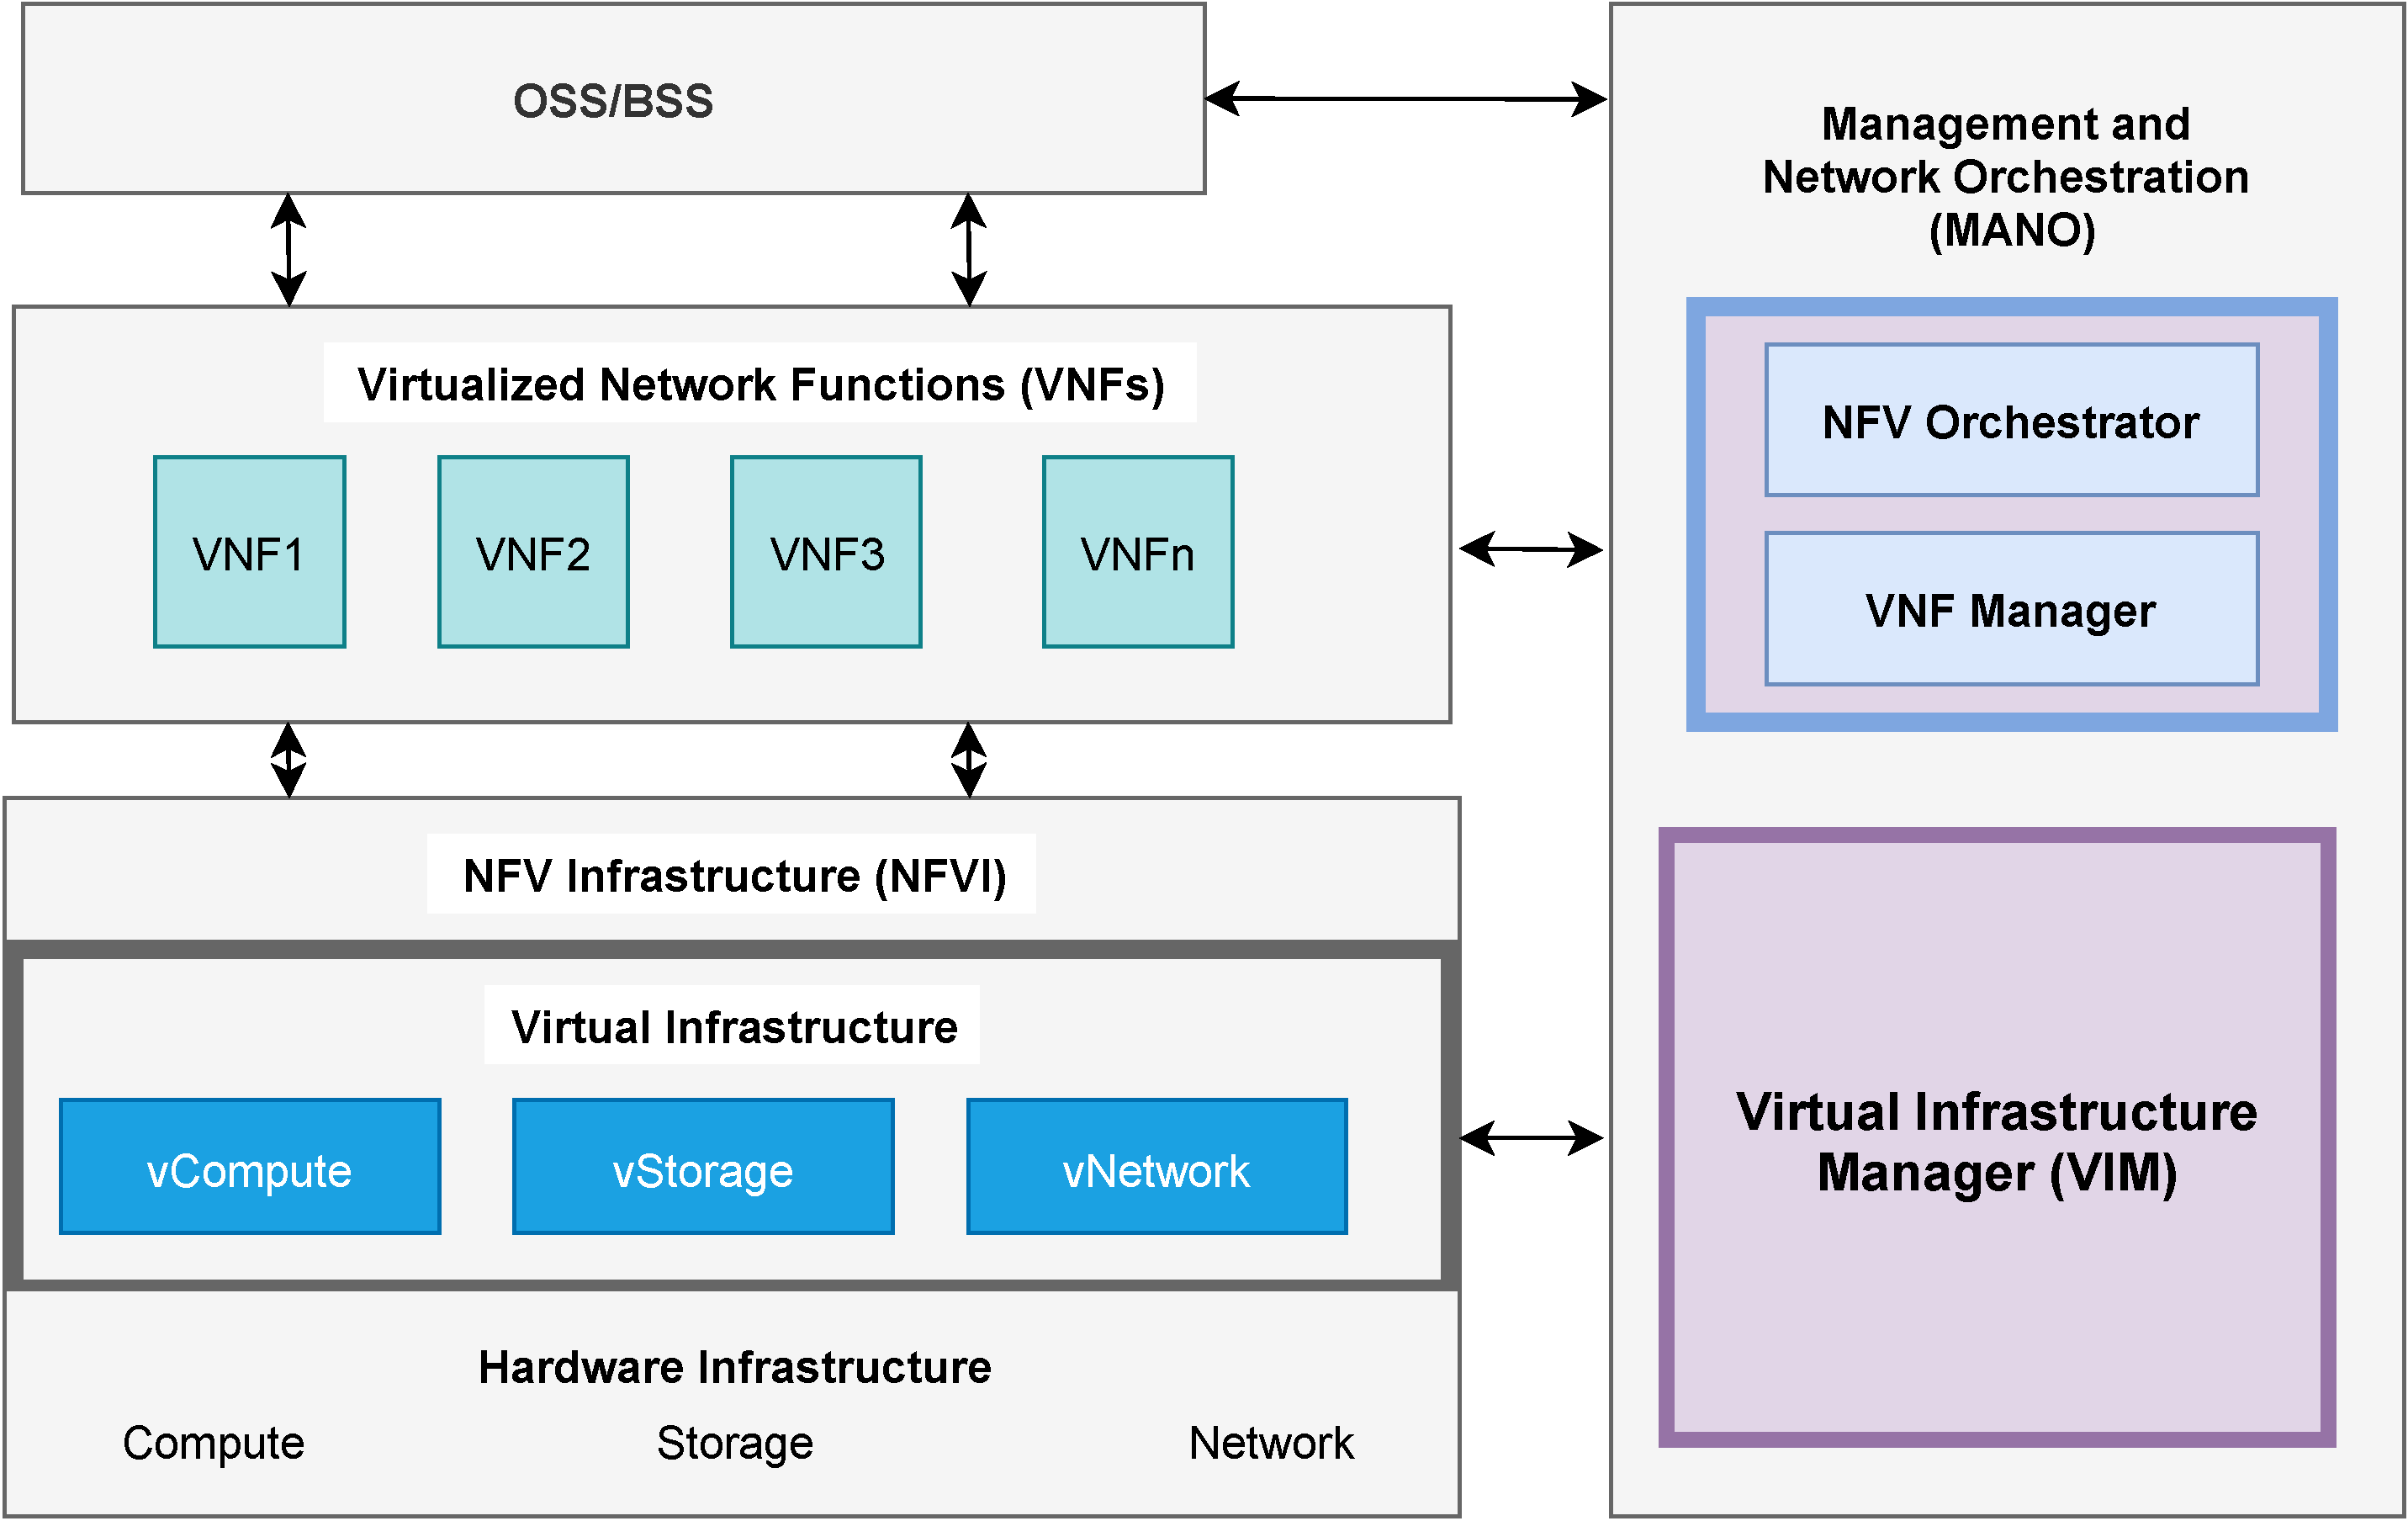
\includegraphics[width=0.78\columnwidth]{NFV.pdf}
\caption{ETSI NFV architectural framework.}
\label{NFV}
\end{figure}\vspace{-12pt}


\begin{figure}[H]%[H]
%\centering
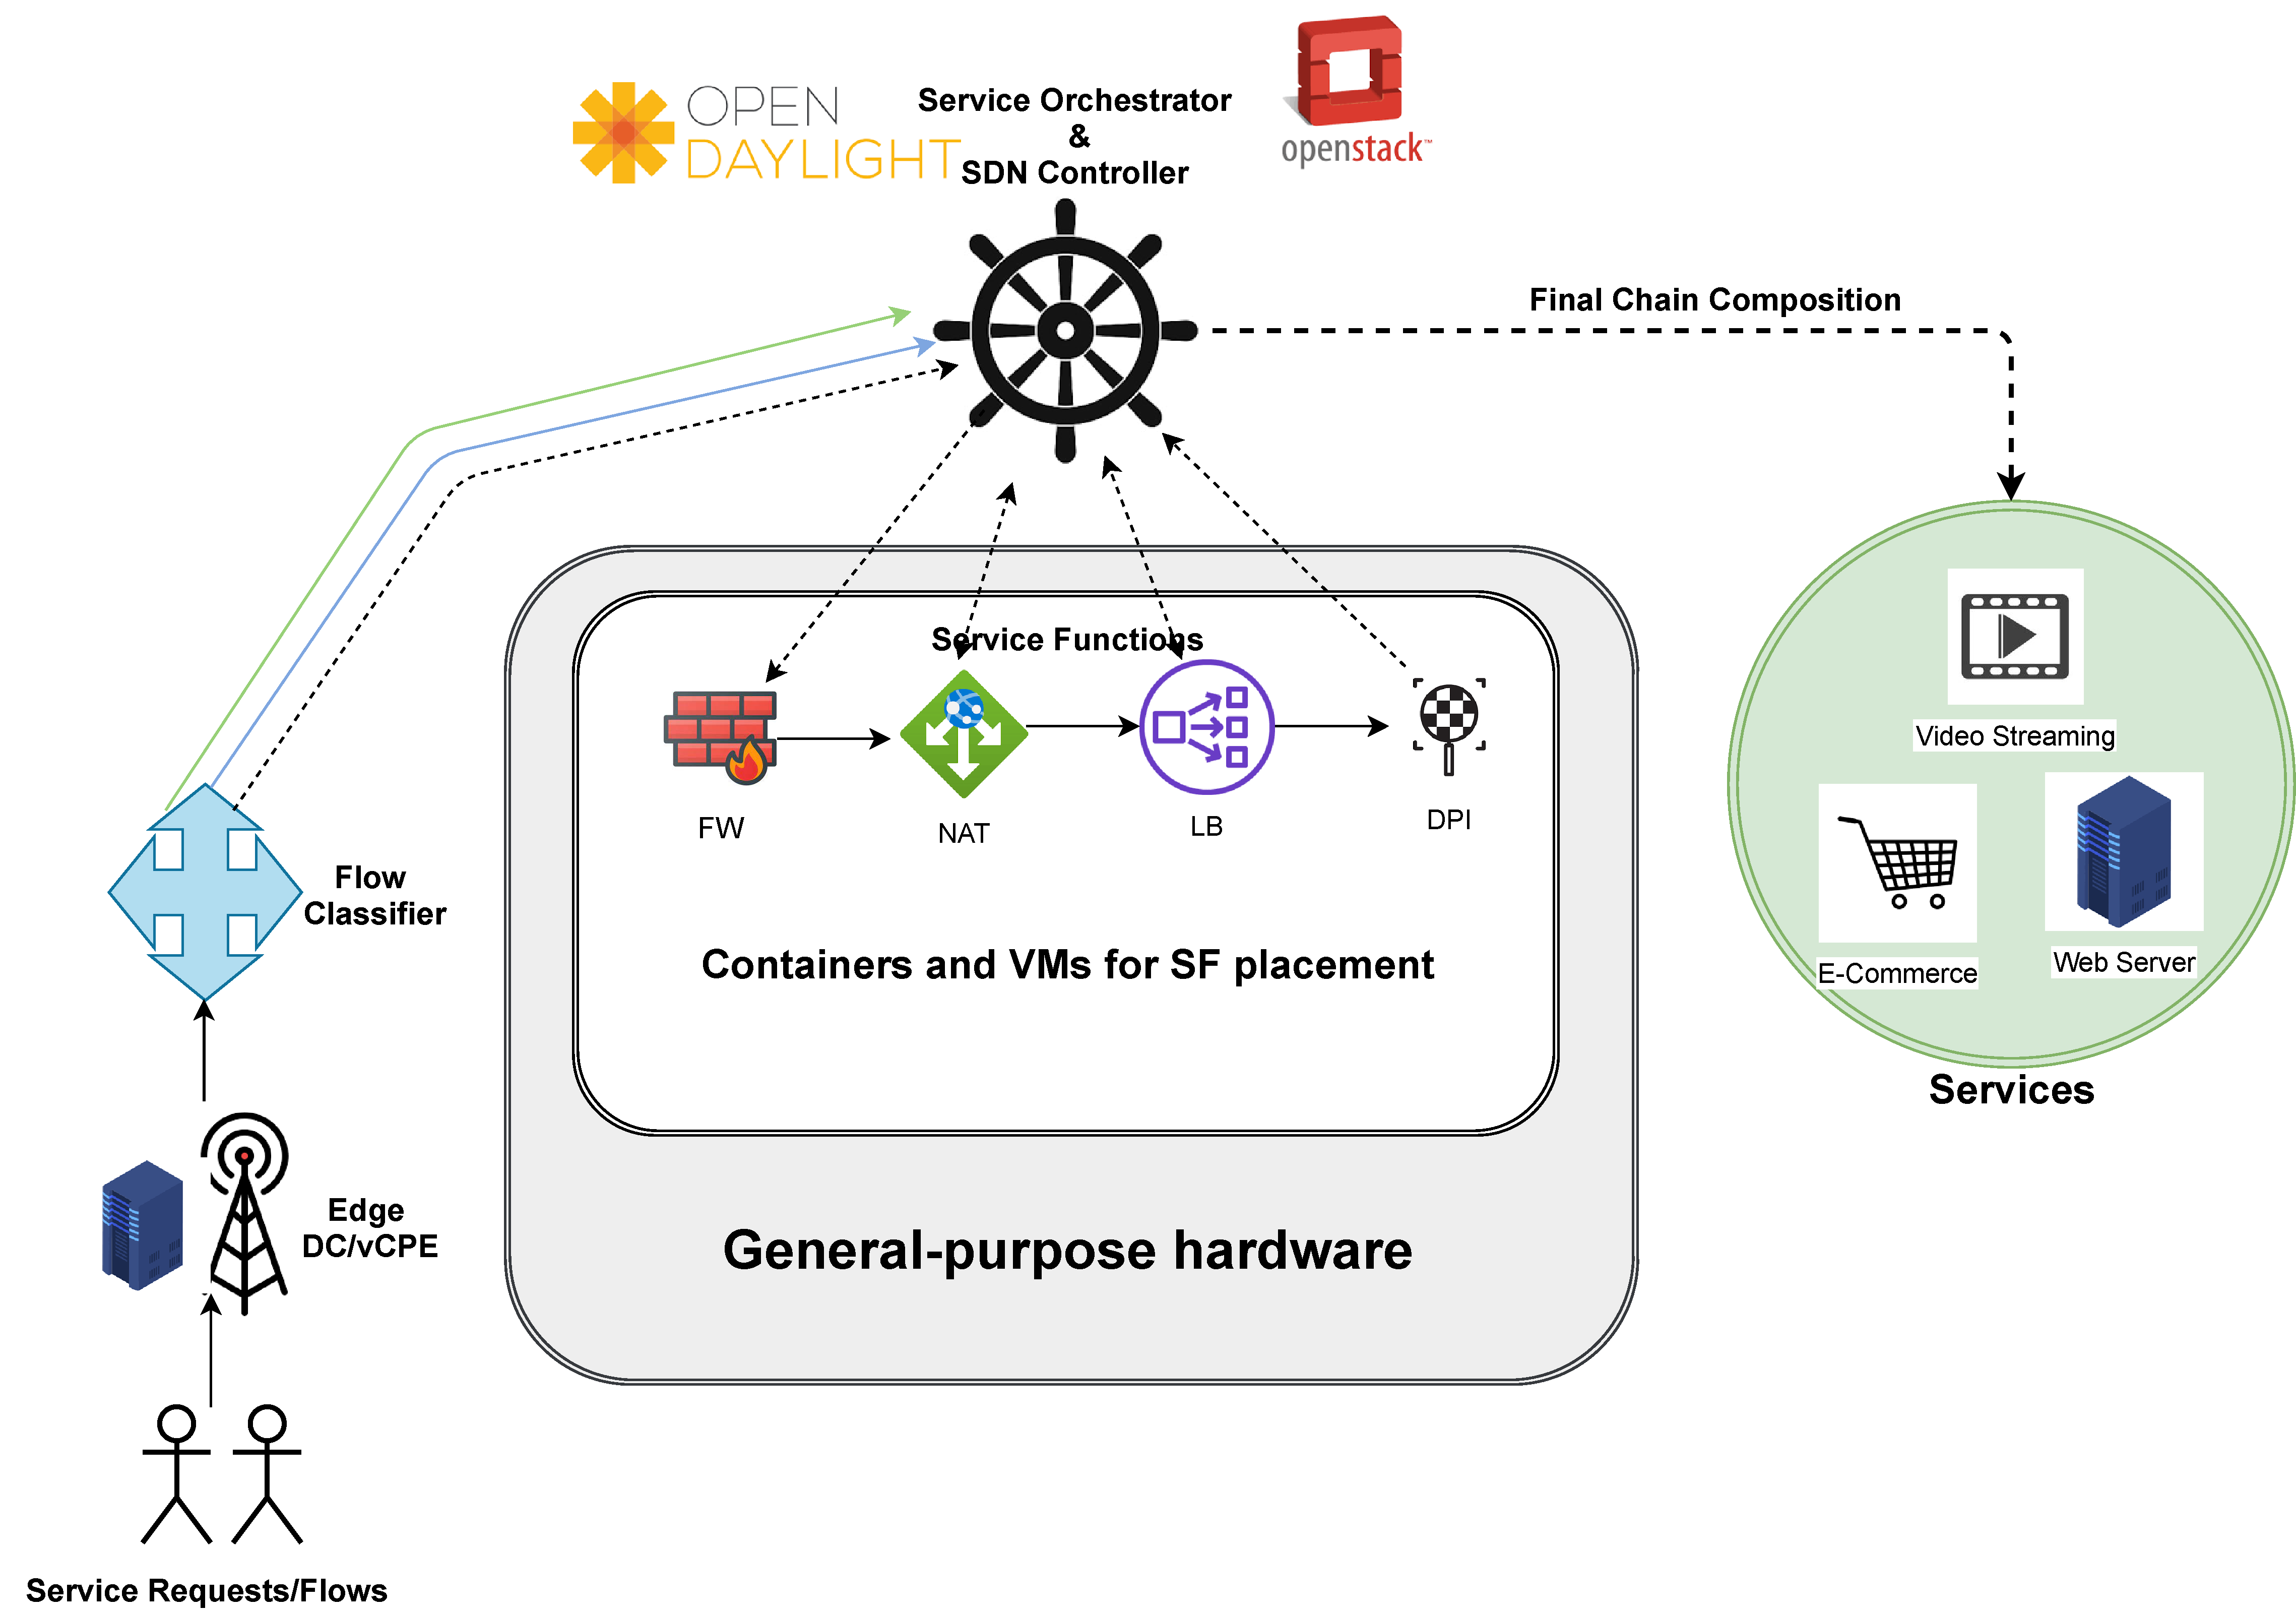
\includegraphics[width=0.97\textwidth]{SFC.pdf}
\caption{Service function chaining scenario.}
\label{Service Function Chaining}
\end{figure}


%%%%%%%%%%%%%%%%%%%%%%%%%%%%%%%%%%%%%%%%%%%%%%
\subsection{Service Function Chaining}
\label{SFC}
The vNFs implemented in NFV constitute the NF forwarding graph, which consists of network functions connected via logical network links to achieve the goal of packet processing by the vNFs. SFC is made up of NFs connected in a chain (based on service requirements and specifications) to deliver end-to-end services to end users~\cite{etsi2013network, wang2021availability}. A typical service chain consists of NFs such as a NAT function, a firewall, and a traffic load balancer. As briefly introduced in Section \ref{SFC-environments}, in order for an SFC deployment to be complete, components such as the service classifier, SFF, Service Function Path, SFC proxy, and service function need to be in place. 

%%%%%%%%%%%%%

%%%%%%%%%%%%%%%%%%%%%%%%%%%%%%%

The IETF SFC architecture presented by Halpern {et al.}~\cite{halpern2015service} shows that the SFCs are either bidirectional or unidirectional, where packet processing is performed through an ordered list of service functions in a unidirectional scenario~\cite{halpern2015service}. A bidirectional SFC scenario requires packet processing elements (SFs) to be placed in both directions of the service chain. SFCs are deployed as network service graphs with SFs placed carefully at different parts of the service chain. The ability to add and remove SFs dynamically along the service path is essential for the design of any SFC framework. NFV and SDN are integrated to achieve instantiation, management, and orchestration of service chains~\cite{ozdem2021subscriber}. 

Intelligent service orchestration is important when handling various service functions, and this can be achieved when the NFV is properly integrated with SDN~\cite{li2015software}. \mbox{Figure \ref{Service Function Chaining}} depicts a typical SFC scenario with service requests generated by users based on the application requirements. A classification of the user traffic is carried out by the flow classifier, which helps in deciding what network function(s) need to be traversed by the traffic before reaching its destination. In a scenario where the service requests traverse more than one NF, a service orchestrator is used to create a chain of NFs that forms the final processing pipeline toward the destination (requested service). 

%%%%%%%%%%%%%%%%%%%%%%%%
\subsection{NFV/SFC and 5G Networks}
\label{5G-Networks}

The chaining of virtual network functions for effective end-to-end service delivery is a key enabler of Beyond 5G networks~\cite{yousaf2017nfv, kak2021towards}. Since 5G-enabled networks are characterized by low latency, programmability, and the support for diverse use-cases of the future, technologies such as NFV can allow providers to deploy services that are suitable for radio access networks (RANs) and mobile core networks~\cite{yousaf2017nfv}.

By implication, using NFV, SDN, and SFC, service providers can easily provide tailored solutions that meet customer demands, by carefully orchestrating user-generated traffic between an ordered list of network functions. As described in Section \ref{SFC-environments}, the chaining of virtual network functions in SFC enables use cases such as the Gi-LAN mobile core network, residential and customer services, and inter and intra-datacentre networks. Other important use cases such as self-driving cars, e-healthcare~\cite{qadri2020future}, and mixed reality (MR) and 5G-enabled IoT~\cite{huang2020effective, qadri2020future} are also possible due to the flexibility offered by 5G network slicing.

Efforts such as the work by Morocho {et al.}~\cite{morocho2019machine} focus on showcasing how machine learning (ML) can be used to leverage the benefits provided by Beyond 5G networks.  ML can be used with enhanced mobile broadband (eMBB) and support future Beyond 5G applications, that are envisaged to have high data rate requirements.  Massive machine-type communications (mMTC) and ultra-reliable low-latency communications (URLLC) are also required to provide support for future use cases for Beyond 5G networks 
\cite{berardinelli2018beyond, katz20186genesis}. 

Abdelwahab {et al.}~\cite{abdelwahab2016network} explored how the 5G RAN can be enhanced using NFV, which could also lead to a reduction in the overall capital expenditure for telecommunications service providers (TSPs). As detailed in~\cite{abdelwahab2016network}, some challenges that are related to 5G networks such as efficient scalability of vNFs between physical networks, vNF performance guarantees, and simultaneously supporting the deployment of hardware and virtualized network functions, can be overcome with the flexibility offered by NFV implementations.
%%%%%%%%%%%%%%%%%%%%%%%%%%%%%%%%%%%%%%%



%%%%%%%%%%%%%%%%%%%%%%%%%%%%%%%%%%%%%%%%%
%%%%%%%%%%%%%%%%%%%%%%%%%%%%%%%%%%%%%%%%%
\section{NFV and SFC Frameworks Taxonomy}
\label{SFC implementation frameworks}
In this section, we present the implementation frameworks proposed for NFV/SFC deployments. 
%%%%%%%%%%%%%%%%%%%%%%%%%%%%%%%%%%%%%%%%%

%%%%%%%%%%%%%%%%%%%%%%%%%%%%%%%%%%%%%%%%%%%%%
Some of these implementations are set out to solve specific problems in the SFC domain, such as resource allocation and service orchestration, performance tuning, resilience, and fault recovery. In Section \ref{Open-challenges}, we present and discuss the open challenges that are related to the implementation frameworks discussed.


Figure \ref{Taxonomy} depicts a summary of the taxonomy of the frameworks presented in our work. Resource allocation and service orchestration frameworks deal with the efficient utilization of available resources, by employing techniques such as synthesizing packet processing graphs and offloading packet processing tasks onto smart NICs, while ensuring that traffic is steered to the right network functions in a service chain, and efficiently managing the life-cycle of network functions. 
 
The frameworks presented under the performance-tuning category are concerned with improving the overall performance of SFCs by employing techniques such as modular SFC deployments, the use of lightweight packet processing elements, the use of acceleration frameworks for packet processing, and deep learning techniques to improve the overall chain-wide performance.

The third category in our taxonomy, resilience, and fault recovery, consists of frameworks that handle the problem of fault tolerance in SFC. These frameworks employ techniques such as network function replication and piggybacking of NF state changes across service chains to achieve resilience in SFCs.

Each of the presented frameworks strive to achieve diverse objectives and are hence very often evaluated against different and incompatible baselines. We have therefore chosen to create a taxonomy of the surveyed frameworks to be able to compare, quantitatively and qualitatively, the different works in their own contexts. Rather than forcing a comparison of potentially disjoint performance characteristics between frameworks that could have led to superficial superiority claims, we have carefully described what each framework has been designed to achieve, what technology and approach has been used, and what performance (or other quality) benchmarks have been performed. Frameworks under each category are discussed next.


\begin{figure}[H]%[H]
%\centering
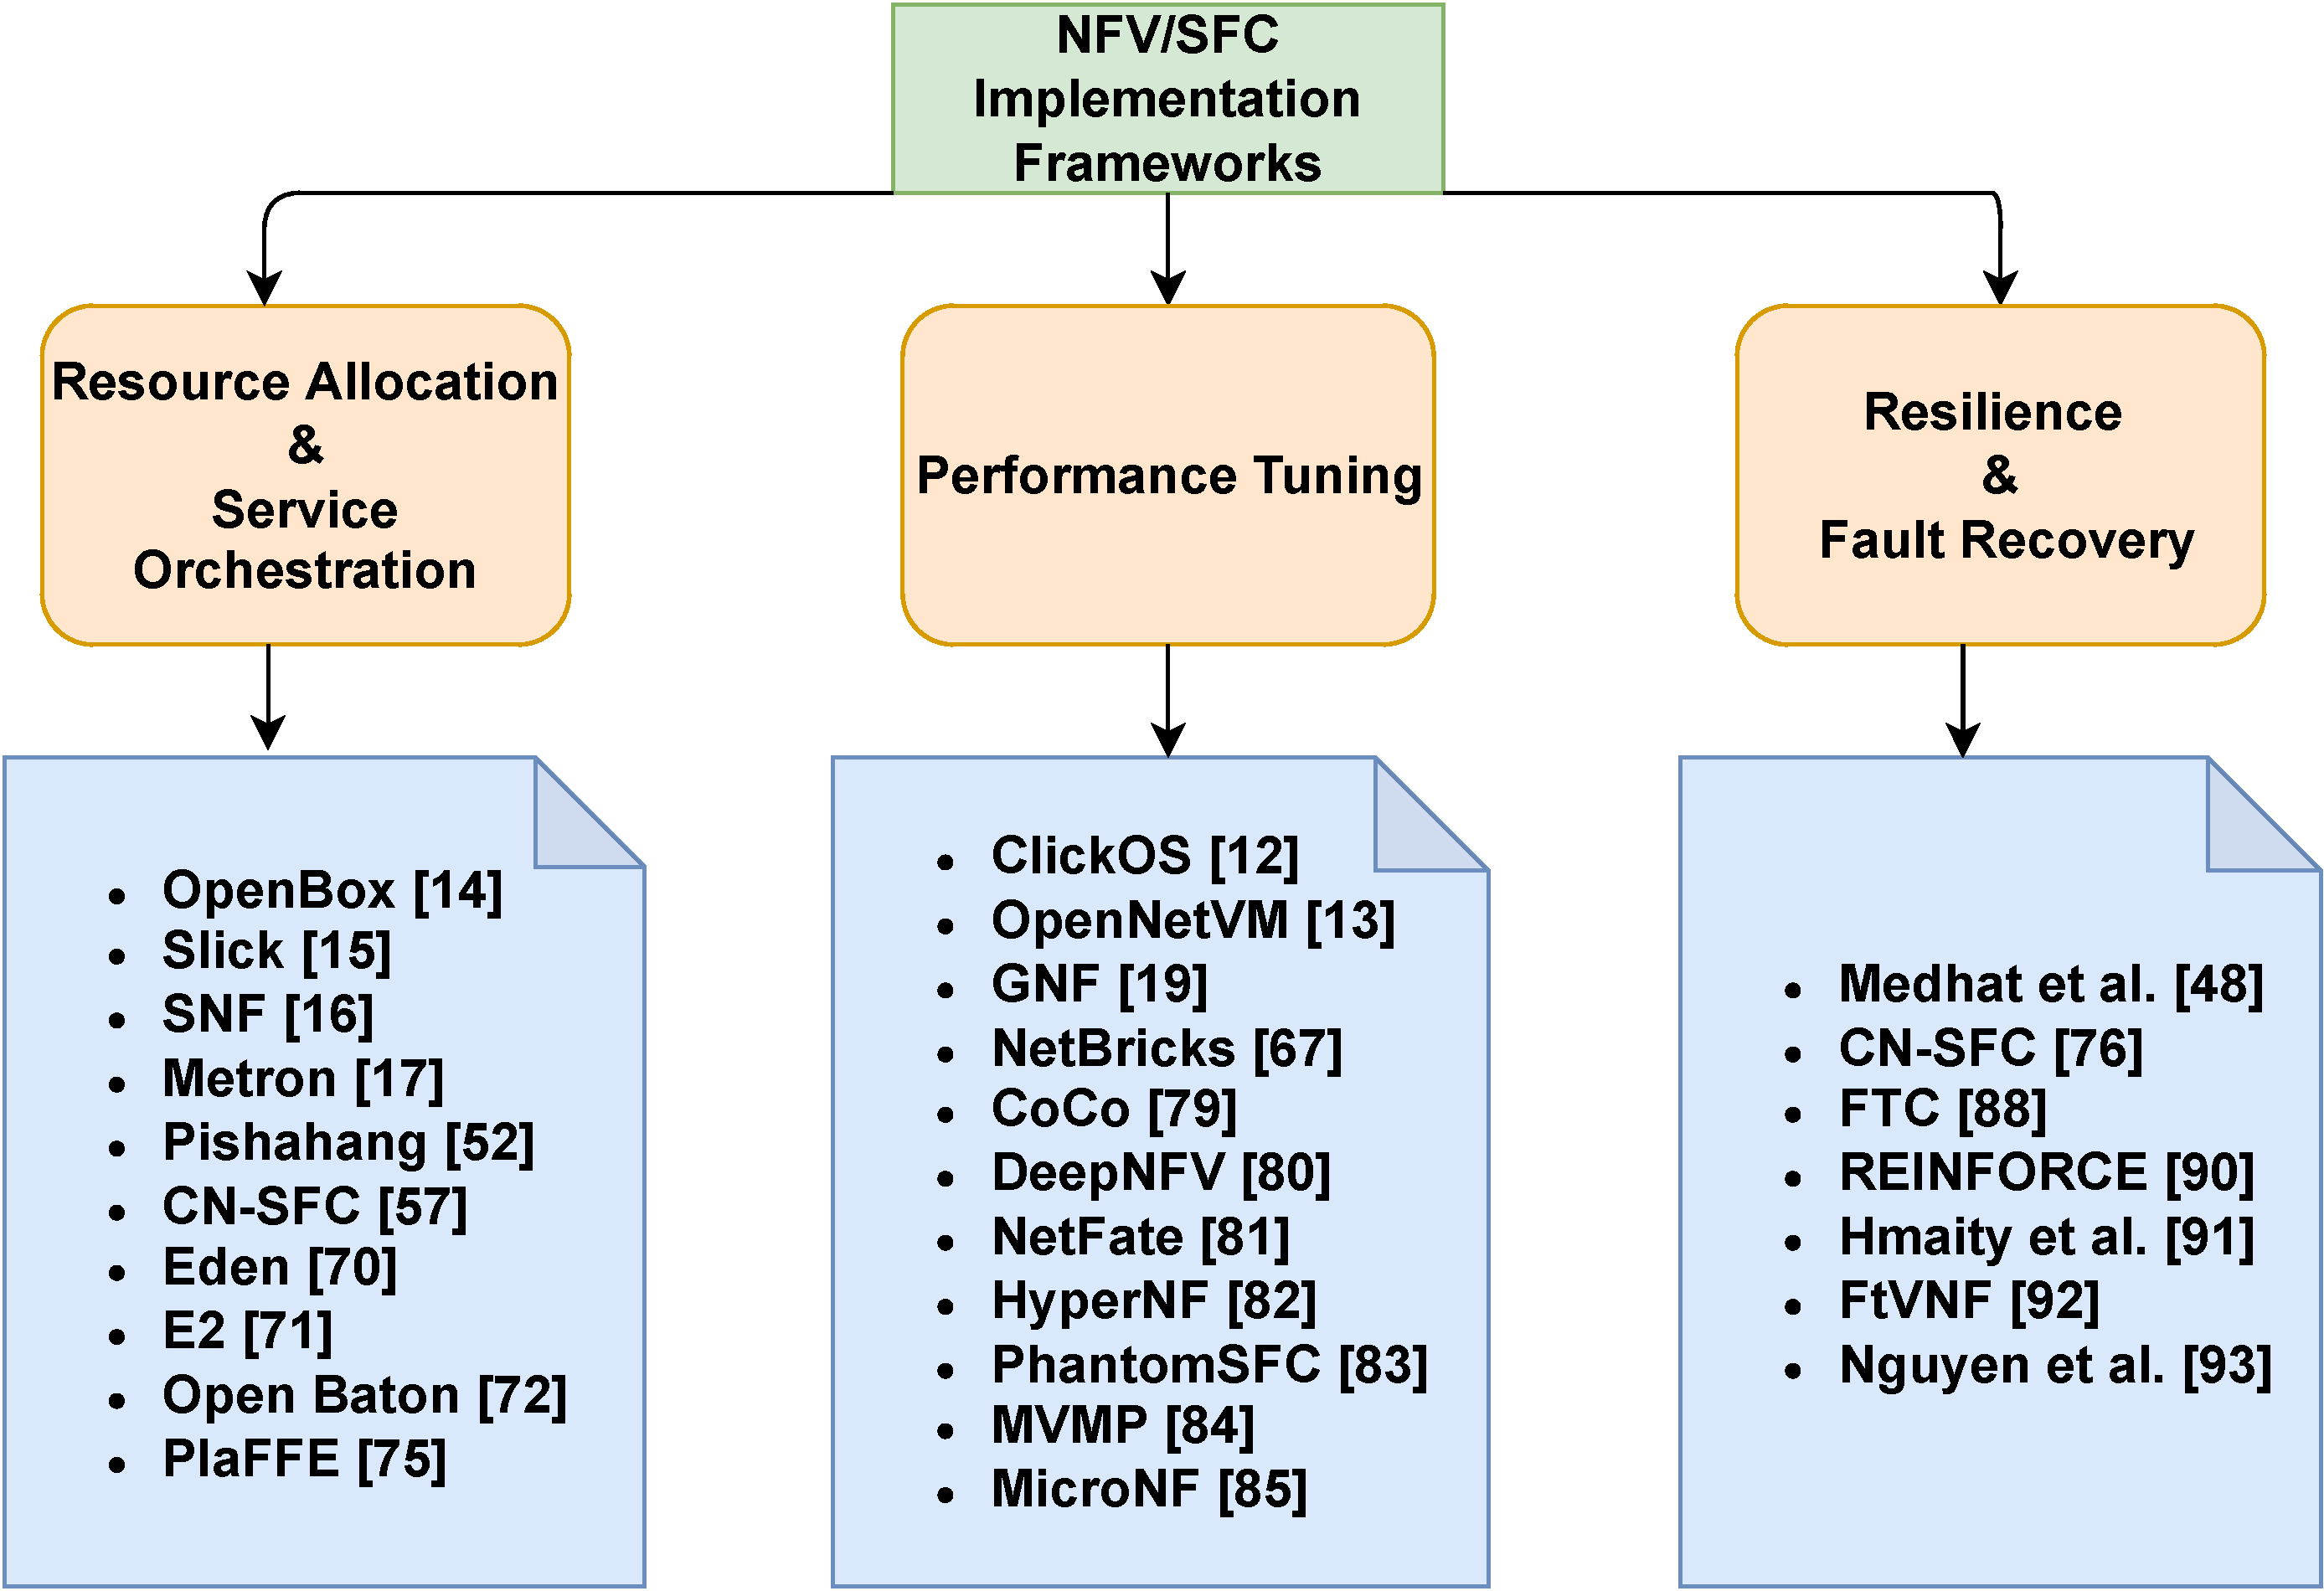
\includegraphics[width=0.8\textwidth]{Taxonomy.pdf}
\caption{{NFV/SFC} %MDPI: References should be cited in numerical order in figure body, please revise it.
 frameworks taxonomy.}
\label{Taxonomy}
\end{figure}
%%%%%%%%%%%%%%%%%%%%%%%%%%%%%%%%%%%%%%
%%%%%%%%%%%%%%%%%%%%%%%%%%%%%%%%%%%%%%
\subsection{Resource Allocation and Service Orchestration Frameworks}
\label{Resource Allocation & Service Orchestration frameworks}
The ability to efficiently allocate network, storage, and processing resources in virtualized network environments is key in service provider networks. This is even more so in NFV/SFC environments, where user traffic type and frequency can either be deterministic or nondeterministic, bringing the need for the underlying system to provide and allocate resources efficiently. The chaining of network functions to provide end-to-end services cannot be achieved without an efficient service orchestration scheme in place~\cite{huang2021scalable}. 
Efforts such as the work by Sun {et al.}~\cite{sun2019low} propose algorithms to handle SFC orchestration, resource utilization, and optimization. The algorithm proposed by~\cite{sun2019low} for example, is based on the breadth-first search (BFS) algorithm, which reduces overall chain-wide latency and bandwidth consumption. This section presents frameworks that have been designed to achieve the goal of efficiently allocating resources in NFV/SFC and the orchestration of network services. We categorically focus on frameworks that handle resource allocation and service orchestration as the core contributions in this subsection of our work by presenting the technologies used and the implementation approach employed by the authors. This has also been summarised in Table \ref{Resource-Allocation-Table}.

%%%%%%%%%%%%%%%%%%%%%%%%%%%%%%

%%%%%%% Resource Allocation
%%%%%%%%%%%%%%%%%%%%%%%%%%%%%%%%%%%%%%%%%%%
\begin{table}[H]
%%\centering
\caption{Resource allocation and service orchestration frameworks.}
\label{Resource-Allocation-Table}
\footnotesize
%\resizebox{\textwidth}{!}{%
	\begin{adjustwidth}{-\extralength}{0cm}
		\newcolumntype{C}{>{\centering\arraybackslash}X}
		\begin{tabularx}{\fulllength}{CCCCC}
\toprule
\textbf{Framework} & \textbf{Problem} & \textbf{Solution(s)} & \textbf{Processing} & \textbf{Testbed/PoC} \\ \midrule


OpenBox~\cite{bremler2016openbox} & vNF provisioning and orchestration  & Lightweight vNFs and decoupling control/data plane. & Click & Mininet \\ %\hline

Slick~\cite{anwer2015programming} & Resource management and efficient traffic steering &vNF placement. & Click & Mininet/VM \\

SNF Framework~\cite{katsikas2016snf} & Resource optimization &  Synthesised processing graphs, stateful NF management and vNF performance optimization.  & Click elements & Servers with MoonGen Packet gen \\ %\hline


Metron~\cite{katsikas2018metron} & Resource Allocation &  Network resource management and server resource utilization. & Click-based & OpenFlow Switch and VM \\ %\hline

Eden~\cite{ballani2015enabling} & Service Provisioning and Orchestration &  End-host NFs, packet offload to NIC and programmable data-plane vNF.  & F\# vNFs & End-hosts and programmable NICs \\ %\hline

E2 Framework~\cite{palkar2015e2} & NF Scheduling and management &  NF placement, effective resource allocation, vNF scaling.  & commodity servers & Hardware switch and servers \\ %\hline

Open Baton~\cite{carella2015open} & NFV/SFC management and orchestration & Network slicing, multi-site orchestration, vNF fault tolerance and resource allocation.  & VMs & OpenStack \\ %\hline

Pishahang~\cite{kouchaksaraei2018pishahang} & Service Orchestration & Multi-domain orchestration.  & VM & OpenStack/Kubernetes \\ %\hline

PiaFFE~\cite{mafioletti2020piaffe} & vNF orchestration & vNF Offloading to eNF, improved throughput and eNF placement. & VM & Servers with SmartNIC \\ %\hline




	\bottomrule
		\end{tabularx}
	\end{adjustwidth}
\end{table}


\subsubsection{Eden Framework}
\label{Eden}
The Eden framework was proposed by Ballani {et al.}~\cite{ballani2015enabling} as a framework suitable for virtual network function provisioning on end-user devices. Eden leverages the concept of data-plane programmability by implementing NFs on end-user devices written in the F\# language, which is a high-level programming language. Eden comprises three functional components that work together to handle packet processing tasks: the centralised logical controller, which is used for service orchestration and for providing a global view of the infrastructure. The second component is the \textit{Stage}, which is simply a name for kernel modules, libraries, or applications on hosts that are used for the classification of packets before being sent to the Enclave (the third component in Eden).

The Enclave is responsible for handling the functionalities of a programmable data plane, which can be implemented on NICs, FPGAs, hypervisors, or operating systems. Eden maintains match-action rules in the Enclave, with traffic association carried out on the host device by the stage component of the framework. The Enclave is also responsible for interpreting the bytecode, which is obtained from compiling action functions. Eden still leaves the open question about where to best deploy the network functions, that is, either on the user OS or on the programmable NIC. In Section \ref{Open-challenges}, we shed some light on this open challenge by arguing for a hybrid implementation framework for fast packet processing and efficient service chain creation in next-generation networks.

%%%%%%%%%%%%%%%%%%%%%%%%%%%%%
\subsubsection{E2 Framework}
\label{E2 Framework}
The E2 framework presented by Palkar {et al.}~\cite{palkar2015e2} is designed for the management of NFV applications and resource allocation, which is achieved without necessarily knowing the low-level implementation of the applications. The target environments for the E2 system are hardware commodity servers and switches in high-performance network environments, which are typically found in today's central office locations. E2 implements a manager, which is responsible for orchestrating communication between the SDN controller and a cluster of servers. 

The E2 framework also manages the placement of NFs using the proposed algorithm on available servers by monitoring the available resources and efficiently placing NFs to avoid unnecessary system overheads. Network operators can define their policies using \textit{pipelets}, which state the steps involved in processing traffic from a specific class. A directed acyclic graph (DAG) is a key component of the E2 \textit{pipelet}, which defines how a class of traffic is processed by the E2 NFs, with nodes representing physical switch ports or NFs. 

The configuration of network functions is done by providing the following inputs: (i) an API exported by E2 for leveraging optimisation options, (ii) a method for attribute association, that is, for per-packet and port metadata; (iii) information on the scalability of the application, that is, whether it can scale across multiple cores or multiple servers, which gives the E2 framework an idea of how to handle situations of traffic overload, (iv)~a method of splitting traffic across multiple NF instances by considering the constraints of the target environment; and (v) information on the NF processing capacity in terms of traffic rate, which helps with placement decisions. E2 provides service providers with the flexibility of declaring their policies without prior knowledge of the underlying network function or infrastructure.         


%%%%%%%%%%%%%%%%%%%%%%%%%%%%%%%%%%
\subsubsection{Pishahang Framework}
\label{Pishahang}
Pishahang is a multi-domain service orchestration framework for SFCs, proposed by Kouchaksaraei {et al.}~\cite{kouchaksaraei2018pishahang,kouchaksaraei2019service} (with the introduction of dynamic service chaining), which combines container-based and VM-based vNFs to create a chain of network services. The framework was implemented across the OpenStack and Kurbenetes domains. In terms of service description, Pishahang uses two descriptors: the first for describing information considered to be \textit{high level}, such as service chaining, microservices, and vNFs, while the second descriptor focuses on a more fine-grained description of vNFs, such as the required resources for running the vNFs. Pishahang is a framework that has been built to chain services across heterogeneous domains. 

Pishahang used the SONATA MANO {\url{https://www.sonata-nfv.eu/}}({accessed} % Please add access date.
on 15 December 2021) 
framework, which supports the addition of new functionalities following a microservice-based architecture. Service graphs are translated by the SDN adaptor, which is sent to the controller, converted to forwarding rules, and installed on switches. To validate the features of Pishahang in chaining services across multiple domains, VM-based and container-based forwarders were chained to create an SFC with ICMP packets sent end-to-end. The use of containers for the deployment of vNFs is yet to be fully developed because of reasons such as lack of functional isolation, and security.


%%%%%%%%%%%%%%%%%%%%%%%%%%%%%%
\subsubsection{SNF Framework}
\label{SNF}
SNF is a SFC framework proposed by Katsikas {et al.}~\cite{katsikas2016snf}, which synthesises SFCs with the main goal of performance optimisation by eliminating redundancy in packet processing across the service chain. Typical causes of redundancy are eliminated by the SNF framework by (i) creating a logical processing entity to handle all chain-wide operations on received packets, rather than handling network functions as separate processes, (ii) discarding packets that need to be discarded very early in the service chain; (iii) reducing multiple read operations by collecting read operations and constructing classes of traffic as a directed acyclic graph, which is synthesised into a classifier, and (iv) reducing the number of write operations by modifying traffic classes in a single operation.

The concept of set theory and graphs is employed for traffic classification to achieve the synthesis of similar network functions to improve the overall performance of the service chain. Another key feature of the SNF framework is the management of states across multiple network functions in a service chain, which enables the synthesis of stateful service chains. At any given time, there is a processing core that actively classifies all the received frames into the required traffic class units. The ingress traffic is hashed using RSS, which helps to serve bi-directional flows by the same processor and re-writer~\cite{katsikas2016snf}.  Figure \ref{SNF-picture} depicts the SNF framework on a device with two network cards, where each NIC is tied to a CPU core.        



%%%%%%%%%%%%%%%%%%%%%%%%%%%%%%%%%%%%

\begin{figure}[H]%[htbp]
%\centering
%\includegraphics[width=0.8\textwidth]{PhantomSFC.png}
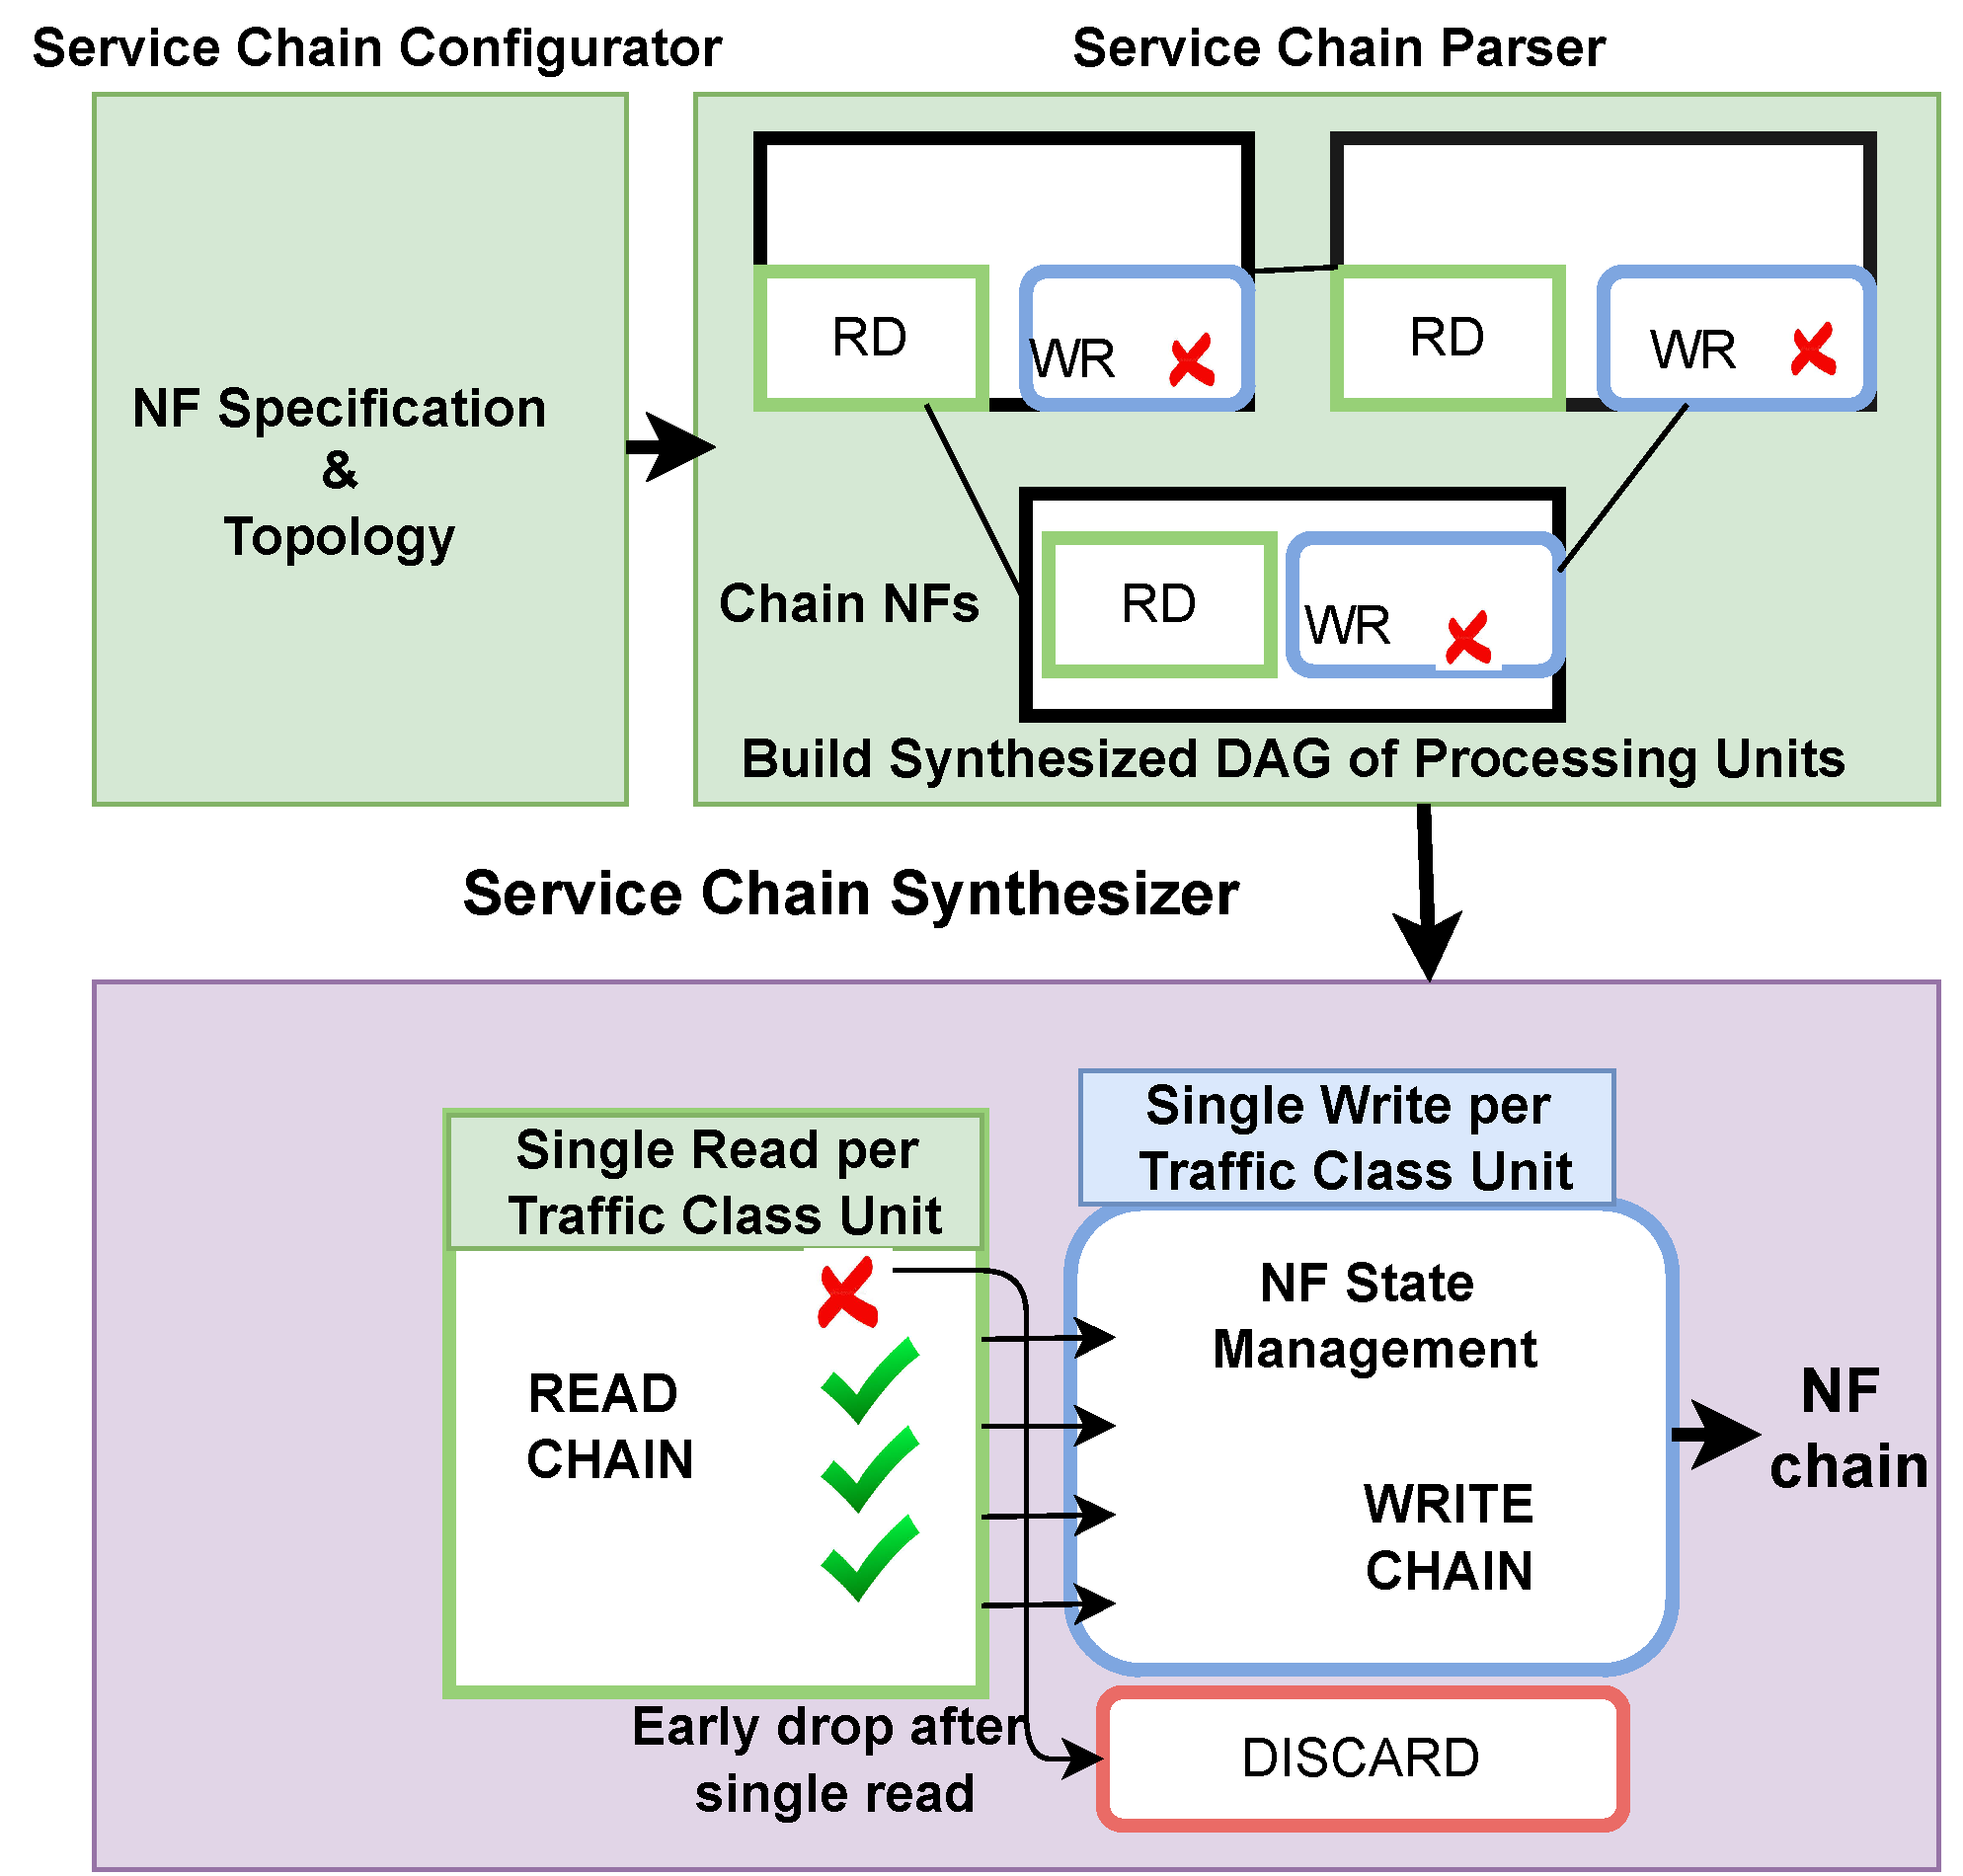
\includegraphics[width=0.6\columnwidth]{SNF.pdf}
\caption{SNF Framework.}
\label{SNF-picture}
\end{figure}

\subsubsection{Open Baton Framework}
\label{OpenBaton}
The Open Baton framework was proposed by Carella {et al.}~\cite{carella2015open} as a framework for NFV service orchestration and management. The framework has the OpenStack cloud infrastructure as its underlying platform, which is compliant with the ETSI MANO architectural framework. The key component implemented by Open Baton is the multi-site service orchestration feature in heterogeneous network environments. Open Baton provides a management component for handling the life cycle of network functions, including the use of the JUJU {\url{http://openbaton.github.io/documentation/vnfm-juju/}} ({accessed} % Please add access date.
on 20 December 2021) virtual network manager for interoperability between diverse network~functions. 

The framework provides support for diverse VIMS, which means there is no need to rewrite the components of the logic that is responsible for service orchestration. To speed up the NF instantiation time, drivers are provided for VIMs and VNFMs that support the deployment of containerized network functions. Scaling of network functions can be handled at runtime using the auto-scaling {component} {\url{https://github.com/openbaton/autoscaling-engine}} ({accessed} % Please add access date.
on 1 January 2022). 

Open Baton  uses {Zabbix} {\url{http://openbaton.github.io/documentation/zabbix-plugin/}} ({accessed} % Please add access date.
on 1 January 2022)  to monitor network activities and network function status. The framework handles resource allocation by leveraging the concept of network slicing using SDN ; thus, the extensibility and interoperability of Open Baton makes it ideal as an orchestration framework for heterogeneous network functions. A fault management module, together with a management dashboard, makes Open Baton a complete solution for heterogeneous NFV orchestration.


%%%%%%%%%%%%%%%%%%%%%%%%%%%%%%%%%%
\subsubsection{Metron Framework}
\label{Metron}
Metron is an NFV framework proposed by Katsikas {et al.}~\cite{katsikas2018metron}, which achieves high utilisation of commodity servers and underlying network resources. Metrons can offload some packet processing tasks to the underlying network infrastructure and achieve low inter-core communication using tag-based hardware dispatching for processing packets. The reduction of inter-core transfers implemented in Metron gives it the capability to process packets at the speed of the L1 cache. Metron performs stateless packet processing and classification by leveraging the OpenFlow and P4 protocols. 

The problem of having a mismatch between the server and network architecture is also addressed by tagging packets to be dispatched and switched in the service chain, which is controlled by the implementation of the ONOS SDN controller. Placement decisions of synthesised packet processing graphs are carried out accurately and at a low cost by obtaining the network state. A load-balancing scheme was introduced for servers and CPU cores~\cite{katsikas2018metron}. Figure \ref{Metron-figure} presents an overview of the Metron architecture, with an example network function chain and execution steps consisting of a firewall and DPI NF.

%%%%%%%%%%%%%%%%%%%%%%%%%
\begin{figure}[H]%[htbp]
%\centering
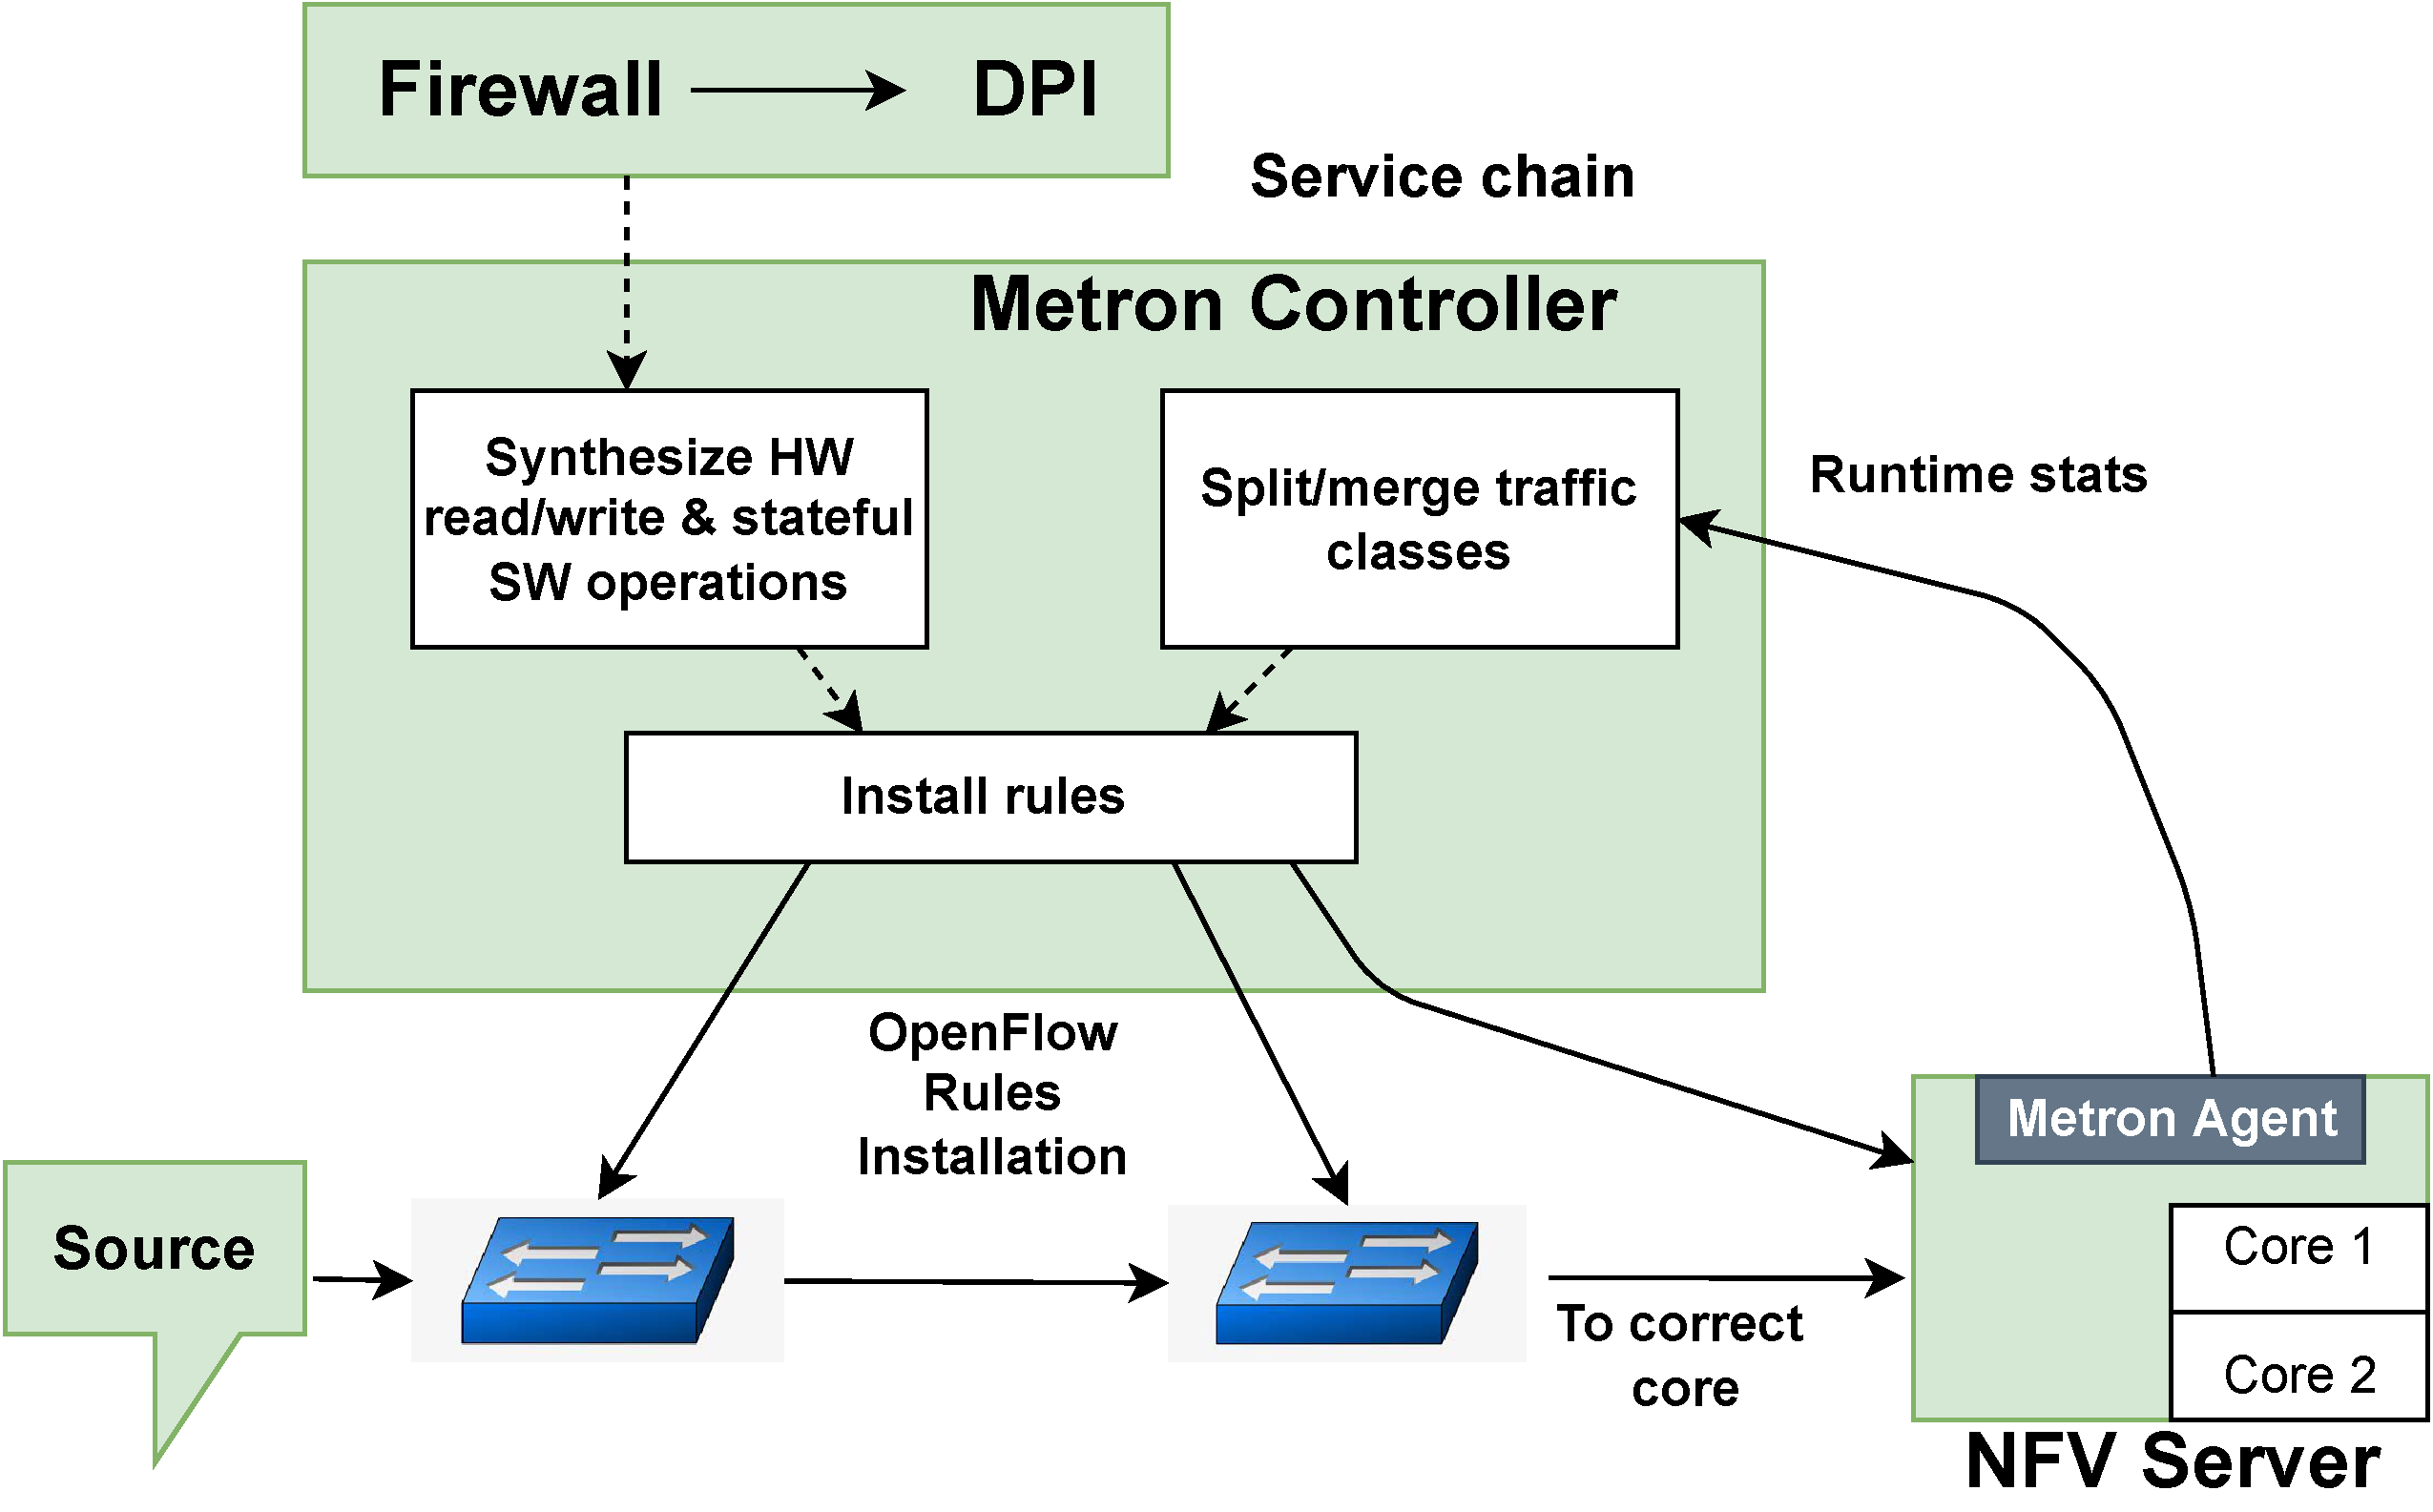
\includegraphics[width=0.8\columnwidth]{Metron.pdf}
\caption{Metron framework overview.}
\label{Metron-figure}
\end{figure}
%%%%%%%%%%%%%%%%%%%%%%%%%%


%%%%%%%%%%%%%%%%%%%%%%%%%%%%%%%%
\subsubsection{CN-SFC Framework}
\label{CN-SFC}
Dab {et al.}~\cite{dab2020efficient} presented an SDNLess SFC microservice architecture for Cloud-Native NFV, a framework for cloud-native SFC creation which uses an advanced version of network service mesh (NSM) {\url{https://networkservicemesh.io/}} ({accessed} % Please add access date.
on 27 December 2021) and Kubernetes {(\url {https://kubernetes.io/})} ({accessed} % Please add access date.
on 2 January 2022) for chaining cloud-native elements to form a service chain. They considered the use of SFCs in micro-service architectures and addressed the shortcomings of the NSM architecture, such as its inability to handle L2 or L3 traffic and the lack of support for advanced routing algorithms.

The cloud-native framework, CN-SFC, was also used to achieve traffic steering by efficiently load-balancing traffic across the Cloud-native functions (CNFs). An approach was introduced, which uses the weighted round robin algorithm by maintaining the weights of Kubernetes pods and distributing traffic based on pods with high weight values. TS-CNF, which is a traffic steering problem, was modelled and solved as an integer programming (IP) problem.

In terms of the evaluation of CN-SFC, a Kubernetes cluster was used, which consists of an NSM control plane, a master node, and two worker nodes. The Docker and the Kind {\url{https://kind.sigs.k8s.io/}}  ({accessed} % Please add access date.
on 28 December 2021) framework were used to run the cluster. The proposed network-aware traffic steering scheme (NA-TS) was evaluated by varying the number of flows that need access to the network service in the cluster. The number of replicas that were used for deploying the VPN and firewall services were also varied, while UDP and ICMP (to evaluate reachability) packets were generated and evaluated (jitter and packet loss in the service chain) between the two assigned pods and those deployed in the cluster. Additional metrics such as the latency of the network and service instantiation time were also evaluated. 


%%%%%%%%%%%%%%%%%%%%%%%%%%%%%%%%%%%
\subsubsection{Slick Framework}
\label{Slick}
The Slick framework was proposed by Anwer {et al.}~\cite{anwer2015programming}, which allows for the programming of network functions with a control program that describes how packets can be processed in a specific traffic set. Traffic flow is specified by applications that provide information on the elements that need to be traversed by the packets in the network. The controller deploys the selected processing elements and deploys them on the machine. The task of resource management in the framework is handled by the slick-run-time, which ensures that the links and processing elements are not overloaded with packets beyond~capacity. 

Network functionalities are placed as software elements, which can be installed dynamically or at the initialisation time. Events are sent to the Slick controller by the modular processing elements; thus, Slick takes care of the placement of network functions and the steering of traffic between packet processing elements. In terms of evaluation, the proposed framework was evaluated using a Mininet SDN network emulator with various network topologies. The controller was run on a separate VM, while the emulator was run on another VM with 60 SDN switches. Both VMs had  eight CPU cores. One of the goals of Slick, which was achieved, is to maximise bandwidth utilisation between various network~functions.

Slick allows the network programmer to use a high-level language to describe a module that handles the steering of traffic, as well as the placement of lightweight functions in arbitrary locations along the service chain. Slick does not consider other environments, such as the edge of the network ; thus, their implementation is restricted to data-center~\mbox{environments}. 

%%%%%%%%%%%%%%%%%%%%%%%%%%%%%%%%%%%%%
\subsubsection{Openbox Framework}
\label{OpenBox}
The OpenBox framework proposed by Bremler {et al.}~\cite{bremler2016openbox} is a framework for the management, development, and deployment of vNFs. OpenBox abstracts network functions as packet processing graphs, which represent the behaviour of typical network functions, such as a firewall, DPI, and NAT. Processing graphs are implemented using the elements of the click router framework~\cite{kohler2000click}, specifically for firewall, web cache, load balancer, and IPS. 

To improve performance, OpenBox introduced a graph merging algorithm to merge the abstracted NF processing graphs, which reduces per-packet latency by minimising the number of processing blocks that need to be traversed by packets. The graph merging process starts by normalising the graphs into trees to avoid the convergence of paths, and the resulting trees are concatenated in the right order of packet processing by the network functions (to ensure chain-wide correctness of the processing pipeline).

There are three major components that make up the OpenBox framework: OpenBox Applications, OpenBox Controller (OBC), OpenBox Service Instances, and OBIs, which constitute the OpenBox data-plane. Packet processing graphs are sent down to the OBI data plane (which can be implemented in hardware or software) from the controller, which in turn receives information about the packet processing capabilities of the OBIs. The communication between the OpenBox controller and the data plane is handled by the OpenBox protocol, which defines packet processing blocks for building vNFs.

The controller is used by OpenBox to achieve multi-tenancy, smart NF placement, and NF scaling, in addition to steering traffic to the right vNF. This component of the OpenBox framework provides network application developers with a layer of abstraction for creating applications that have a specific packet processing graph and logic. The OpenBox framework was evaluated using service chain configurations and pipelined network function scenarios, with both scenarios yielding much higher throughput when compared with scenarios without OpenBox. To cater to the resilience of network functions, the authors merged multiple NFs together to create a single processing pipeline, which provides higher throughput to one of the network functions at off-peak times of the second NF in the merged processing graph, yielding a throughput that is 20\% better than the naive merge approach.  


%%%%%%%%%%%%%%%%%%%%%%%%%%%%%%%%%%%
\subsubsection{Piaffe Framework}
\label{PIaFFE}
PIaFFE, a Place-as-you-go in-network framework for flexible embedding of vNFs, is a placement framework proposed by Mafioletti {et al.}~\cite{mafioletti2020piaffe}, which achieves multilevel chaining and placement of vNFs implemented on SmartNICs. The overall aim of the PIaFFE framework is to maximise throughput and achieve minimum latency by embedding network functions (eNFs) on in-network processors. These embedded network function implementations reduce server CPU utilisation on end-hosts, increase throughput to line rate speeds, and reduce latency.

A PoC which was implemented on two physical servers was achieved by chaining three network functions for authentication, IDS, and firewall functionality. PIaFFE reduces host load by performing full or partial vNF offloading while consolidating multilevel chaining. PIaFFE made use of the P4 programming language to steer traffic to vNFs or eNFs, depending on what function has been embedded as an eNF. This decision is determined by the P4 hash table or bloom filter, which has been implemented using a P4 Data Structure (P4DS).



%%%%%%%%%%%%%%%%%%%%%%%%%%%%%%%%%%
%%%%%%%%%%%%%%%%%%%%%%%%%%%%%%%%%%
\subsection{Performance Tuning Frameworks}
\label{Performance tuning frameworks}
Improving the performance of virtual network functions, either as standalone functions or as part of a service function chain, helps network operators reduce service instantiation costs~\cite{katsikas2021metron}, and the optimal use of available resources. In this subsection, we present frameworks that focus on optimising the performance of network functions in a service chain. Most frameworks that are designed to optimise performance devise mechanisms that can achieve goals such as reducing network function deployment and provisioning time, maximising the throughput of network applications and reducing latency (Table \ref{Performance-Tuning-Table}). We would like to note that there are several efforts in the literature that focus on optimising network functions using diverse technologies and implementation methodologies. We present the state-of-the-art equivalence classes of frameworks in this category by explaining the design, technology, methodology, and results obtained by each framework.


\subsubsection{Coco Framework}
\label{CoCo}
CoCo is an NFV framework proposed by Meng {et al.}~\cite{meng2018coco}, which was designed for the deployment of modularized service function chains (MSFCs). One of the major goals of the proposal is the consolidation of processing elements collocated on a VM and handling the placement of the modularized SFC to minimise packet transfer overhead between VMs. The authors designed a placement scheme that selects the right SFC elements for consolidation using performance and resource-aware placement. Fairness is achieved between several NFs tied to a single CPU core using a run-time scheduler implemented in CoCo. 

In terms of scalability, CoCo can utilise a push-aside scheme specifically designed to handle reduction in performance, which might arise due to scaling elements. Unlike most existing NF scalability approaches that start up a VM when there is a need to scale, which leads to more overhead in terms of latency, the push aside algorithm reduces the need for inter-VM hop creation. Rather than creating a new replica (as used by traditional vNF scalability solutions), the CoCo framework adds more resources to elements that are~overloaded.   

In terms of performance evaluation, the efficiency of resource utilisation and the reduction in the cost of transferring packets across the service chain are the two major benefits of the CoCo framework. Throughput and CPU utilisation were measured with CoCo implemented using Docker containers to allow for the consolidation of processing elements; thus, Open vSwitch was employed as the virtual switch for VM-VM communication. The results show that CoCo can improve performance by approximately 45.5\% and a 2.46X reduction in packet transfer overhead.


\begin{table}[H]
%%\centering
\caption{Performance tuning frameworks.}
\label{Performance-Tuning-Table}
%\resizebox{\textwidth}{!}{%
	\begin{adjustwidth}{-\extralength}{0cm}
		\setlength{\cellWidtha}{\fulllength/5-2\tabcolsep+0.0in}
\setlength{\cellWidthb}{\fulllength/5-2\tabcolsep-0.2in}
\setlength{\cellWidthc}{\fulllength/5-2\tabcolsep+0.7in}
\setlength{\cellWidthd}{\fulllength/5-2\tabcolsep-0.5in}
\setlength{\cellWidthe}{\fulllength/5-2\tabcolsep+0.0in}
\scalebox{1}[1]{\begin{tabularx}{\fulllength}{>{\PreserveBackslash\centering}m{\cellWidtha}>{\PreserveBackslash\centering}m{\cellWidthb}>{\PreserveBackslash\centering}m{\cellWidthc}>{\PreserveBackslash\centering}m{\cellWidthd}>{\PreserveBackslash\centering}m{\cellWidthe}}

\toprule
\textbf{Framework} & \textbf{Problem} & \textbf{Solution(s)} & \textbf{Processing} & \textbf{Testbed/PoC} \\ \midrule

ClickOS~\cite{martins2014clickos} & Middlebox optimization & Optimized packet processing and Zen-based VM optimization. & Click & Xen-based hypervisor \\ %\hline

OpenNetVM~\cite{zhang2016opennetvm} & VNF performance optimization & DPDK-enabled vNFs, containerised NFs, kernel by-pass packet processing and line-rate packet processing. & Containers & DPDK-enabled hosts and containers \\ %\hline

NetBricks~\cite{panda2016netbricks} & NF performance optimization &  Zero-copy isolation and memory level isolation. & VM & Physical servers \\ %\hline


GNF~\cite{cziva2015container} & Edge vNF deployments &  Lightweight vNFs and edge service chains & CN & Host with CNs \\ %\hline


CoCo Framework~\cite{meng2018coco} & Modular SFC & Optimization of modular SFCs, effective resource allocation, resource-aware placement,  vNF fault tolerance and optimized run-time scheduler. & Containers & Commodity servers \\ %\hline

DeepNFV~\cite{li2018deepnfv} & NFV SFC performance & Deep learning for QoS and traffic optimization, lightweight containerised vNFs and Edge NF deployments. & Containers & GNF framework \\ %\hline


NetFate~\cite{lombardo2015open} & Edge NFV deployments & Active NF/VM migration and open PaaS platform. & VM & Commodity servers and virtual switches \\ %\hline

HyperNF~\cite{yasukata2017hypernf} & NFV SFC performance &  Reduced I/O sync overheads, hypercall-based I/O in VM context and vNF scalability.  & VM & VALE switches and VMs \\ %\hline

PhantomSFC~\cite{castanho2018phantomsfc} & Resource optimization  & Service/Control decoupling, reduced latency and improved throughput. & VMs & VM/DPDK \\ %\hline

MVMP~\cite{zheng2018flexible} & NFV SFC performance & Improved throughput, lightweight vNFs, vNF fault tolerance and vNF replication.  & Containers & DPDK, Container, Virtual Switch \\ %\hline

MicroNF~\cite{meng2019micronf} & NFV/SFC performance & Optimal NF placement, reduced inter-NF latency, vNF performance optimization and scalability and fair scheduling of vNFs. & Containers & Docker and VMs \\

	\bottomrule
		\end{tabularx}}
	\end{adjustwidth}
\end{table}

%%%%%%%%%%%%%%%%%%%%%%%%%%%%%%%%%




%%%%%%% Performance tuning
%%%%%%%%%%%%%%%%%%%%%%%%%%%%%%%%%%%%%%%%%%%

%%%%%%%%%%%%%%%%%%%%%%%%

%%%%%%%%%%%%%%%%%%%%%%%%%%%%%%%%
\subsubsection{Deepnfv Framework}
\label{DeepNFV}

DeepNFV is a lightweight NFV framework proposed by Li {et al.}~\cite{li2018deepnfv}, which was designed specifically for edge network deployments, with the aim of minimising the packet processing tasks at the core of the network by offloading to edge network functions. DeepNFV is built on the GNF framework~\cite{cziva2015container}, which uses lightweight docker containers to build network functions for the edge. The key components of the proposed framework are the deep learning models employed and the infrastructure layer, which handles the interaction between network links and devices.

DeepNFV uses deep learning to enhance tasks such as the optimisation of QoS parameters, classification of traffic, and analysis of network links. Similar to the GNF framework, DeepNFV was built to support the idea of moving network processing elements as close to the data source as possible (edge computing). As a use case for the DeepNFV framework, network traffic analysis functionality was considered by the authors by generating basic images from network traffic. A traffic analysis-containerized network function was used for the analysis and classification of images using deep learning models. 

To demonstrate the traffic analysis use case, the DeepNFV framework starts by splitting the received traffic into discrete components, which are stored as PCAP files,  and the second step involves the modification of the packet headers to trim the header length or remove unimportant fields from the packets. The modified PCAP files are \textit{cleaned} to remove duplicates before being converted into image data. The resulting images are processed by the CNN model and sent to the next network function in the chain for further action(s). The ability of the framework to classify images and the performance of the network functions at the edge of the network were evaluated, and improved performance in terms of precision and efficiency was recorded. 


%%%%%%%%%%%%%%%%%%%%%%%%%%%%%%%%%%
\subsubsection{Micronf Framework}
\label{MicroNF}
The MicroNF framework was proposed by Meng {et al.}~\cite{meng2019micronf} as a framework for the deployment of modularized service chains, using a centralised controller for service chain graph reconstruction and redundant NF reuse. Service providers describe the MSFC to be deployed by clearly defining how the elements are interconnected. This is followed by processing the MSFC using graph reconstruction and the identification of any dependencies by elements, with the aim of reusing elements where possible. The reordered MSFC is optimally placed with the goal of reducing the latency between processing elements.

The major goals of the framework are to (i) efficiently reuse elements that have similar configurations in the processing pipeline by first addressing the problem of dependency between different elements, (ii) solve the problem of VM to VM connection using a virtual switch in an optimal fashion, (iii) shorten the service chain length, and reduce packet processing costs, where necessary.

In terms of the scalability of NFs, MicroNF implements run-time scaling algorithms, which ensure minimal inter-NF latency along the service chain. The problem of selecting processing elements that are ideal for consolidation is also handled by the MicroNF framework, in addition to a placement algorithm that prioritises high performance. The speed of packet processing between diverse elements is also  considered by the proposed resource scheduler, which ensures that the workload is efficiently shared among available processing elements~\cite{meng2019micronf}.  

%%%%%%%%%%%%%%%%%%%%%%%%%%%%%%%%%%%%%%%
\subsubsection{Netbricks Framework}
\label{NetBricks}

NetBricks is an NFV framework proposed by Panda {et al.}~\cite{panda2016netbricks}, which offers a platform for building and running virtual network functions that provide software isolation between NFs. The NetBricks framework differs from other approaches by (1) limiting the set of processing modules to core functionalities, which helps to reduce the number of modules that network application developers must deal with, and (2) allowing the customization of modules using user-defined functions, which makes the modules more flexible and optimised for better network function(s) performance. 

NetBricks eliminates overheads resulting from context-switching by enforcing memory-level isolation in software and reducing I/O related overheads by introducing zero-copy software isolation~\cite{panda2016netbricks}. Using zero-copy isolation, the cost of packet I/O is greatly reduced by NetBricks, which means that chains of network functions can be run as a single process. 

NetBricks provides a major distinction in providing fault and memory isolation for NF implementations by utilising operators designed for parsing, de-parsing, transforming, and filtering packets. In addition to packet operators, the framework also provides abstractions for processing byte-streams, abstractions for control flow, and for state and scheduled events. To evaluate the performance of the NetBricks framework, two example network functions were used: the first is a simple network function that decrements the TTL of a packet and discards any packet that has a TTL of 0,  and the second is a stripped down implementation of the Maglev load balancer~\cite{eisenbud2016maglev}, which splits ingress traffic among servers and also provides failure recovery for back-end servers. 

The measurements evaluated include simple NF overheads, array bound overheads, and how \textit{general} the NetBricks programming abstractions can be. For the latter part of the evaluations, that is, the programming abstractions, five network functions were implemented: NAT, firewall, Maglev load balancer, and a Snort-like NF that performs signature matching on ingress packets. Improved performance was observed for scenarios where (1) CPU cores and chain lengths were varied, (2) the load was varied with respect to CPU cycles and chain length, and (3) throughput measurements for single network functions with a variable number of CPU cycles for multiple isolation approaches.


%%%%%%%%%%%%%%%%%%%%%%%%%%%%%%%%%%%%
\subsubsection{Hypernf Framework}
\label{HyperNF}
HyperNF is a high-performance NFV platform proposed by Yasukata {et al.}~\cite{yasukata2017hypernf}, which aims to properly  utilise commodity server resources while scaling the number of network functions hosted by servers. The problem space addressed by HyperNF includes resource allocation, efficient utilisation, and high throughput when using everyday commodity servers to deploy virtual network functions.

The proposed framework is aimed at large NF deployments, where utilisation is maximised for better throughput. The use of hypervisor-based I/O is employed, which helps reduce synchronisation overhead. HyperNF was designed using three core design objectives: (i) CPU cores are not reserved entirely for virtual I/O operations, thus providing high flexibility in terms of utilisation, (ii) proper accountability for virtual I/O tasks on respective VMs, thus offering a cohesive resource allocation strategy, and (iii) VM switches should not be used for packet switching; instead, the data path of software switches is exported to the hyper-visor for the purpose of forwarding and switching of packets.

HyperNF was evaluated for scenarios involving a baseline setup using the VALE~\cite{eisenbud2016maglev} switch for inter-VM communication, with each VM tied to a single CPU core, and second, a scenario that consolidates network functions in a shared CPU environment by varying the number of VMs (CPU cores are shared among the firewall VMs deployed using a round-robin scheme). Both scenarios outperformed the split and merge schemes compared with HyperNF. Other tests carried out include resource allocation, NFV throughput, and SFC chain composition. A chain of 50 NFs can achieve a delay as low as 2 ms, which makes the framework ideal for SFC deployments.


%%%%%%%%%%%%%%%%%%%%%%%%%%%%%%%%%%%%%%%%
\subsubsection{Netfate Framework}
\label{NetFate}
NetFate was proposed by Lombardo {et al.}~\cite{lombardo2015open} as a framework that supports the deployment of network functions at the network edge and data centre infrastructure. The main elements of the NetFate framework are simply the clients, which receive or generate packets, and the CPE nodes, which hosts the network functions for clients to connect to the~infrastructure. 

The orchestrator contains an SDN controller for handling communication with OpenFlow switches, an NFV coordinator for handling VM life-cycle and hypervisor-VM communication, and an orchestration engine which collects statistics about available devices, connected clients, and network services. Each time ingress packets are received, the orchestrator (i) takes a decision on which NFVI can host the NF based on defined SLA, (ii) carries out the migration or instantiation of VMs for hosting the NFs in (i), (iii) creates a virtual service path for connecting VMs that host the NFs, (iv) forward ingress flows based on defined routing policies, and (v) terminating unused VMs, thus making resources available. 

The Proof of Concept employed for the evaluation of NetFate comprises client devices and nodes that represent network access points, a controller, and an orchestrator which also authenticates and authorises users. This was made possible by the implementation of two firewall network functions at CPE nodes, where migration efficiency is measured while moving from one CPE node to the other. The NetFate framework is ideal for customer premise equipment network function deployments; thus, its performance in terms of provider equipment implementation is yet to be evaluated.


%%%%%%%%%%%%%%%%%%%%%%%%%%%%%%%%%%%%%%%%%
\subsubsection{Clickos Framework}
\label{clickOS}

ClickOS was proposed by Kohler {et al.}~\cite{martins2014clickos}, which uses the \textit{elements} from the Click software router~\cite{kohler2000click} to achieve lightweight middlebox packet processing. This runs on Linux VMs and an XEN-based {\url{https://xenproject.org/users/virtualization/}} ({accessed} % Please add access date.
on 4 December 2021) optimised platform. To achieve domain isolation, each click middlebox is run on a separate Linux VM, which provides memory isolation. ClickOS achieves high performance in terms of network I/O by making the following changes to the Xen network pipe: (i)~replacing the OvS backend switch, which makes it easier to map VM memory, (ii) moving the netback driver to the control plane, which serves as a communication medium with the netfront driver, and (iii) modifying the netfront driver of the VM to allow the mapping of ring buffers. The framework presented some useful modifications to the Xen backend and frontend modules to achieve faster data transmission rates. 

The evaluation results show that ClickOS speeds up networking for Xen-based VMs by applying several well-known optimisation approaches, such as removing unnecessary data paths and batching of processes. The performance of the ClickOS switch was measured, in addition to metrics such as boot time, memory footprint, throughput, delay, chaining, scalability, and middle-box state insertion. An increased throughput from 8 Kp/s to 344~Kp/s was achieved by changing the driver settings, receiving grants for buffers at the initialisation time, and re-use the buffers for all packets. The VALE switch, which is an in-kernel virtual switch in Linux that allows for scalability in terms of the number of ports and throughput, was replaced by Open vSwitch. 



%%%%%%%%%%%%%%%%%%%%%%%%%%%%%%%%%%
\subsubsection{Opennetvm Framework}
\label{OpenNetVM}

The OpenNetVM framework was developed by Zhang {et al.}~\cite{zhang2016opennetvm} as a framework that is ideal for high-performance vNF deployments using the Intel Dataplane Development Kit (DPDK) {\url{https://www.dpdk.org/}} ({accessed} % Please add access date.
  on 8 December 2021) and Docker Containers {\url{https://www.docker.com/}} ({accessed} % Please add access date.
on 17 December 2021). To achieve high-speed packet I/O transfer, OpenNetVM implements zero-copy to reduce the I/O overhead associated with copying packets from the NIC for processing in the user space. Packets are DMA'd directly from the NIC to a shared memory space, which is accessible to DPDK-based network functions supported by the framework.

%%%%%%%%%%%%%%%%%%%%%%%%%%%%%%

%%%%%%%%%%%%%%%%%%%%%%%%%%%%%%%%

As depicted in Figure \ref{OpenNetVM-Figure}, a shared memory space is created by the manager, which stores the metadata information, list of service chains, and flow tables. Dependencies are encapsulated in Docker containers that host the network functions; thus, packet transfer between NFs is handled by the TX and RX threads that carry useful descriptors. High-speed packet processing is also made possible by utilising the DPDK poll-mode driver rather than~interrupts. 

In terms of NF-to-NF communication, OpenNetVM  uses a centralised logical controller, which communicates using the OpenFlow protocol to orchestrate NF activities. The network function manager is responsible for managing memory and the NF life-cycle by handling inter-NF communication and sending keepalive messages. The transfer of packets between the NICs and NFs is also handled by the manager using the TX and RX threads. Network functions are either implemented using DPDK or as a user-space container process, which are tied to specific CPU cores in both scenarios. The framework was evaluated using metrics such as the scalability of multiple ports, overflow of the flow director, performance of service chains, and the flexibility of the framework can steer packets, which yields a much better performance when compared with ClickOS, especially in terms of throughput with variable chain length.

\subsubsection{Phantomsfc Framework}
\label{PhantomSFC}
PhantomSFC was proposed by Castanho {et al.}~\cite{castanho2018phantomsfc}, which is an SFC framework aimed at decoupling the underlying network from the service plane. The design was implemented to be transport-independent, network agnostic, elastic, and maintains a small footprint by considering end-to-end throughput and latency. The PhantomSFC framework is based on the IETF SFC reference architecture presented by~\cite{halpern2015service}, which comprises a classifier, an SFF, SF, and a proxy component. NSH, which was standardised by~\cite{quinn2018network}, was used as the encapsulation protocol for SFCs in PhantomSFC.

Components such as proxies, forwarders, and classifiers are deployed as vNFs, and a centralised SDN controller is employed for the realisation of chain configuration and instantiation. Tasks involving chain configuration, such as creating a new chain and removing and modifying configuration rules in proxies, classifiers, and forwarders are carried out by the logically centralised controller. Using PhantomSFC, resources can be scaled by SPs based on service demands; thus, the PoC evaluation of PhantomSFC achieved improvements in throughput, jitter, and latency, using the DPDK application.


\begin{figure}[H]%[htbp]
%\centering
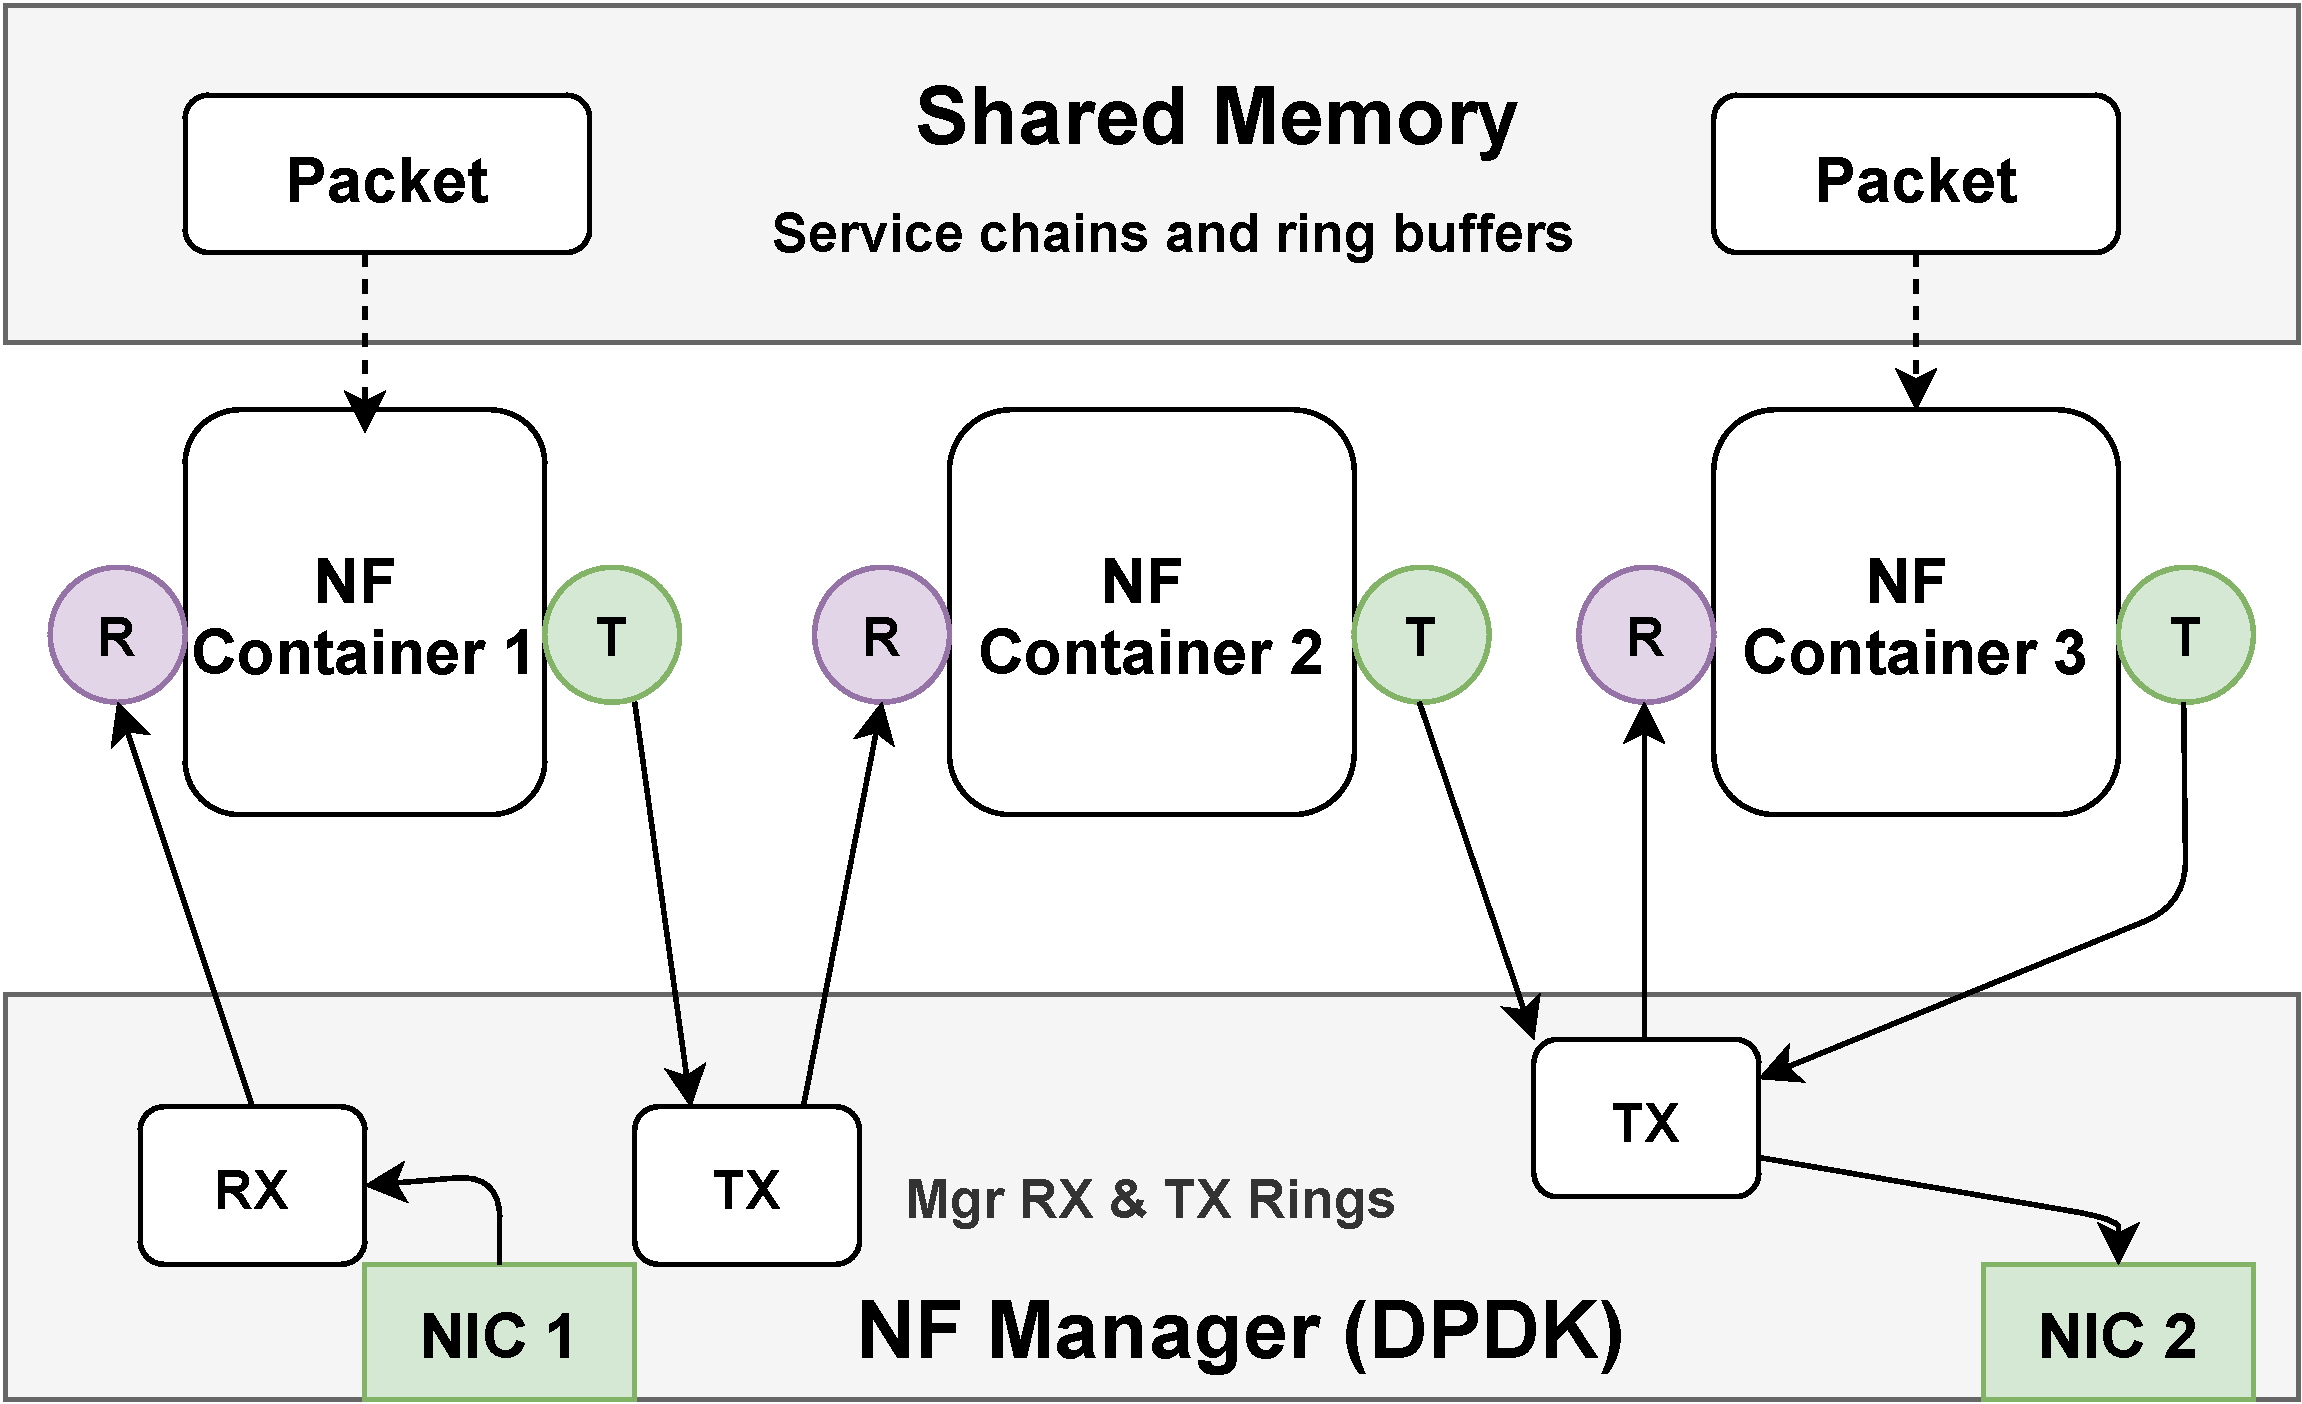
\includegraphics[width=0.85\columnwidth]{OpenNetVm.pdf}
\caption{OpenNetVM framework.}
\label{OpenNetVM-Figure}
\end{figure}


%%%%%%%%%%%%%%%%%%%%%%%%%%%%%%%%%%%%%%%%%



%%%%%%%%%%%%%%%%%%%%%%%%%%%%%%%%%%%%%%%%%
\subsubsection{GNF Framework}
\label{GNF}
The Glasgow Network Functions (GNF) framework was proposed by Cziva {et al.}~\cite{cziva2015container} as an open and lightweight implementation framework for network functions in OpenFlow network environments. GNF, which is a container-based framework, achieves low overhead in terms of performance, high NF reuse, and fast deployment speed, when compared to most NFV deployments. To achieve the routing of traffic in a typical NFV scenario, policies can be implemented by adding entries or by adding a middle-box in the path of the traffic. These two approaches have drawbacks that the GNF framework attempts to eliminate.

GNF achieves dynamic placement of network functions by simply rerouting the traffic to the server with the requested NF, which allows service providers to utilise the same hosts when handling network and compute functions, thus minimising the overall infrastructural costs. Using the OpenFlow protocol, GNF can match ingress packets to the match-action table before routing packets to the specified destination. 

For ease of network function deployment and management, GNF provides a user interface for global control and view of the network, a manager, GLANF router, and agent. The life cycle of network functions is handled by the GLANF Manager, which makes use of the OpenDaylight SDN controller for performing tasks such as creating, starting, stopping, and deleting primitives (Figure \ref{GNF-figure}). Tasks such as resource allocation are also handled by the manager, which allocates network functions to hosts that have available resources. 

To evaluate and demonstrate the performance of the GNF framework, six network functions were deployed: a wire, which routes packets from its ingress to egress ports, an HTTP filter, traffic control, a load balancer, intrusion detection, and a firewall, which is based on iptables. Figure \ref{GNF-figure} depicts the GNF framework, with packets sent from VM1 to VM2, which are sent via the network functions on the GLANF system and to target hosts. The performance of GNF was also compared to ClickOS~\cite{martins2014clickos}, which shows a significant improvement from 3.6 Gb/s to 13.8 Gb/s packet processing speeds, this also holds true as the number of chained containerised vNFs are increased.


%%%%%%%%%%%%%%%%%%%%%%%%%%%%%%%%%%%%%%%%%
\begin{figure}[H]%[htbp]
%\centering
%\includegraphics[width=0.8\textwidth]{PhantomSFC.png}
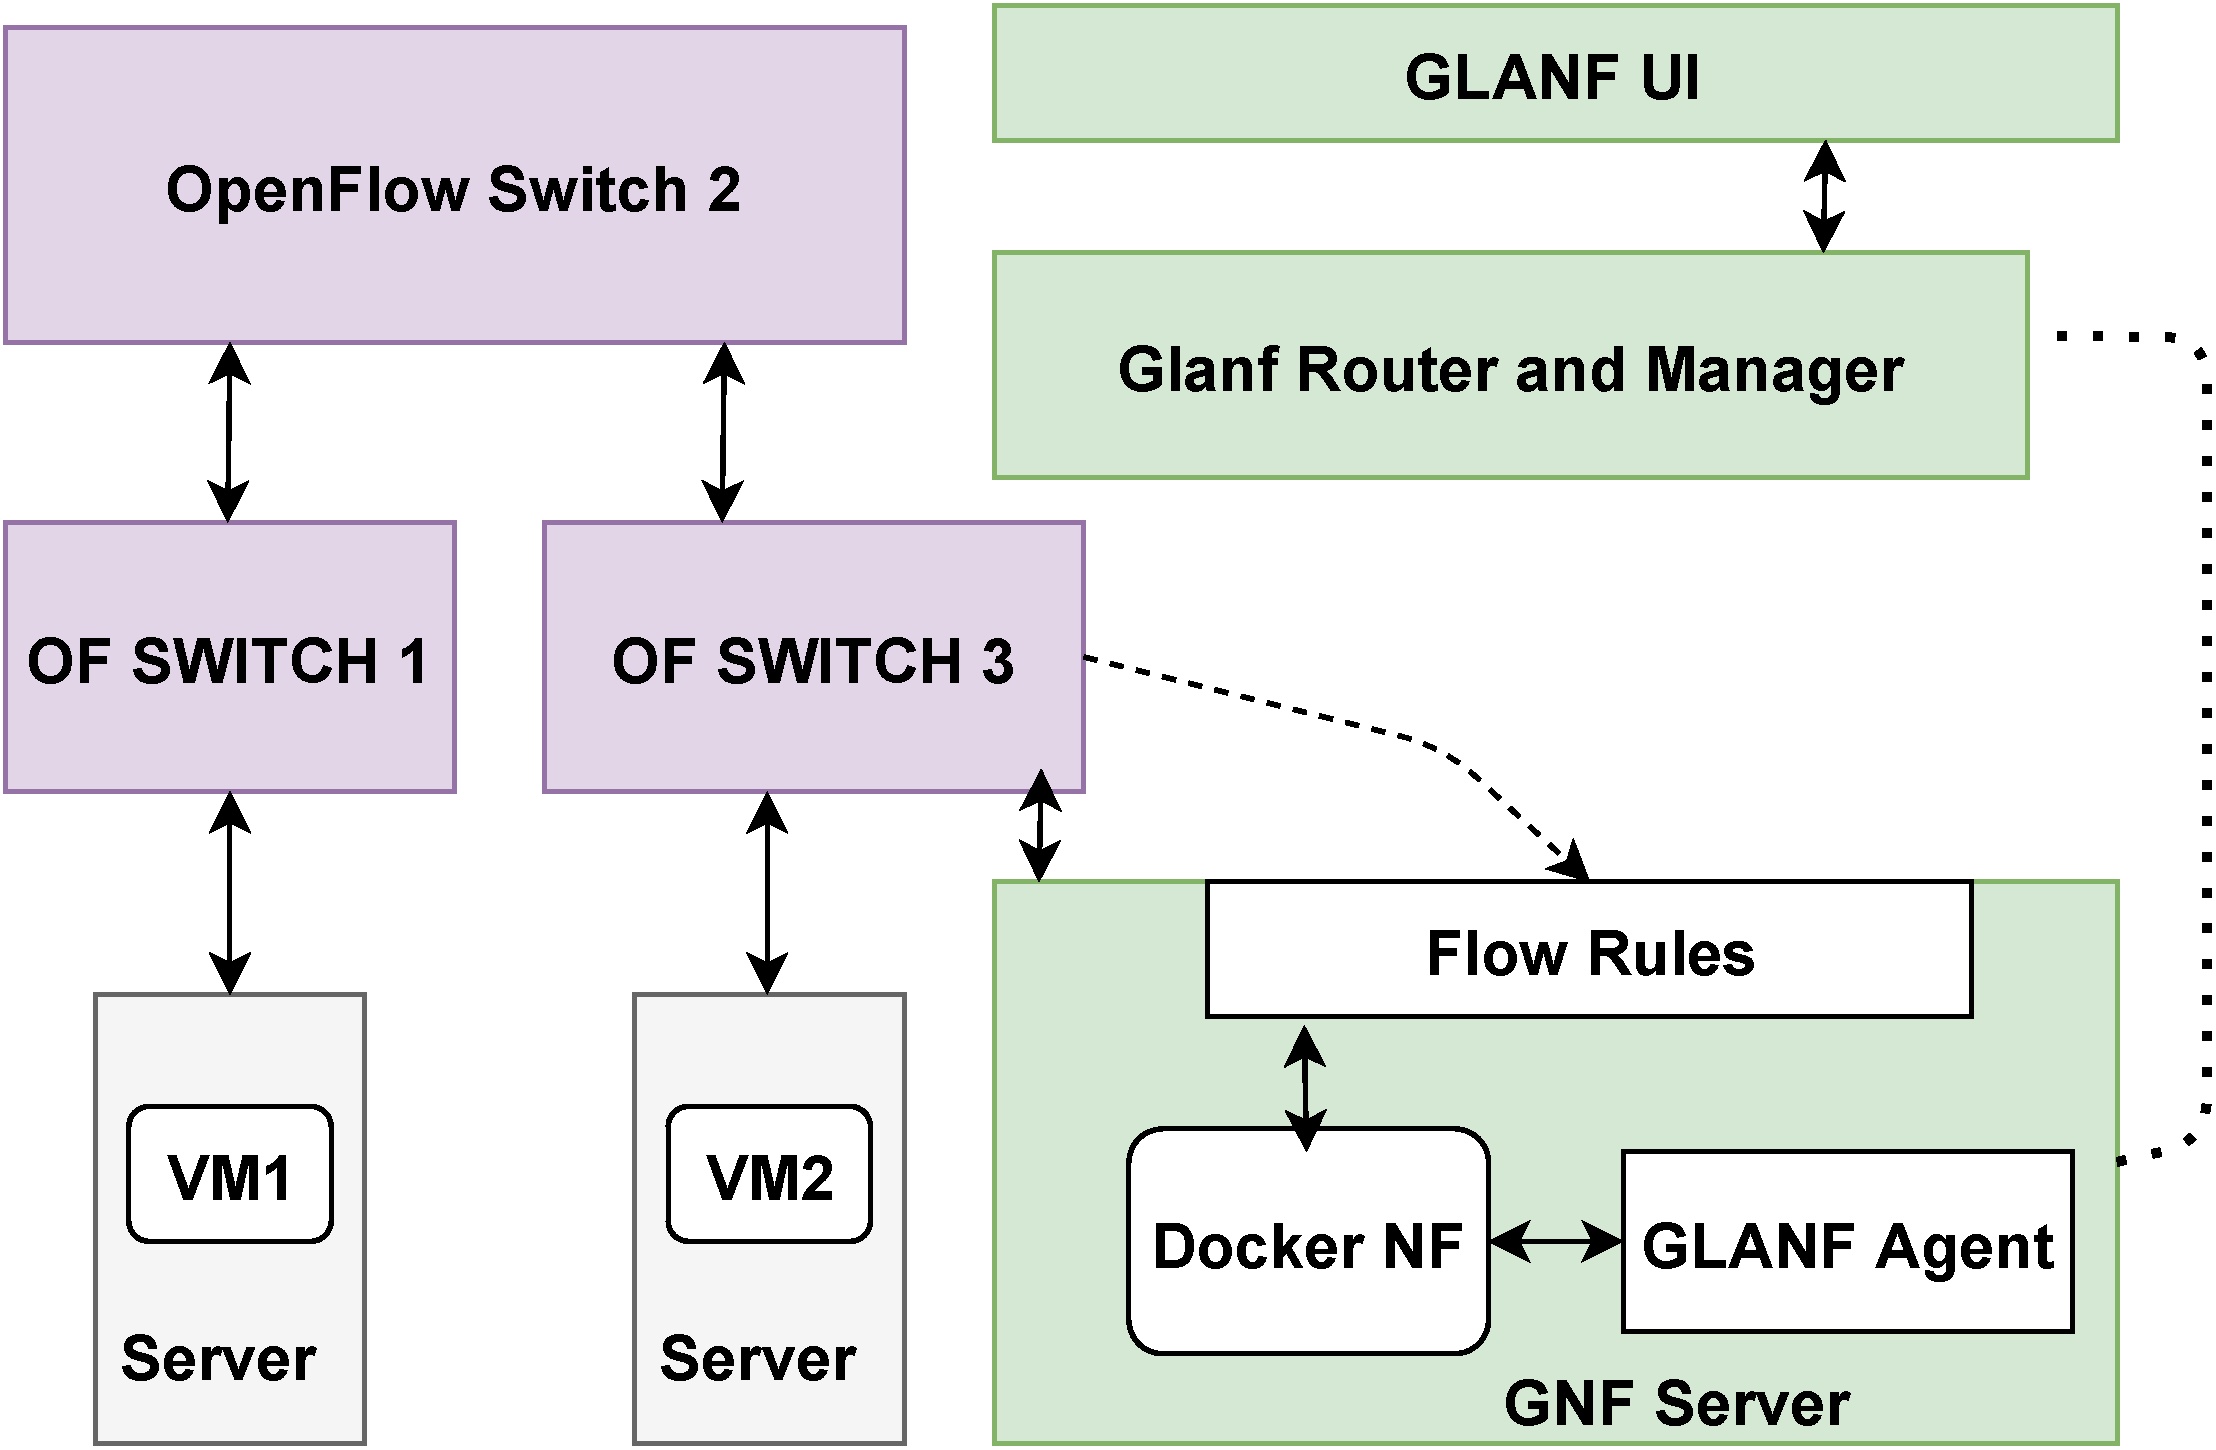
\includegraphics[width=.9\columnwidth]{GNF.pdf}
\caption{GNF architecture.}
\label{GNF-figure}
\end{figure}
%%%%%%%%%%%%%%%%%%%%%%%%%%%%%%%%%%%%%%%%%%%


%%%%%%%%%%%%%%%%%%%%%%%%%%%%%%%%%%%%%%%%%%%%%%%%%%%%
\subsubsection{MVMP Framework}
The NFV platform proposed by Zheng {et al.}~\cite{zheng2018flexible}, i.e., the Multiple Virtual Middlebox Platform (MVMP) is a high performance framework that has been built using the Intel DPDK platform and Docker containers. The three major components of the proposed MVMP framework are (i) abstracted virtual devices, (ii) a control plane, and (iii) a shared memory space. Packet processing by NFs is achieved by an abstraction layer that supports the deployment of multiple NFs on a single hypervisor. Network functions are run in user space as processes, which makes them lightweight, thus requiring fewer resources for packet processing. Packets are polled directly from the NIC using the DPDK poll mode driver and sent to several network functions, which also adds to the fast packet processing speed of the proposed framework.

In terms of implementation and evaluation, network functions were implemented and chained together, and the service chain performance was evaluated and compared with the OpenNetVm~\cite{zhang2016opennetvm} framework, which yields 3x better throughput as the number of network functions is increased in the chain, with an overhead of approximately 4\% with regard to network function isolation. 




%%%%%%%%%%%%%%%%%%%%%%%%%%%%%%%%%%%%%%%%%%%%
%%%%%%%%%%%%%%%%%%%%%%%%%%%%%%%%%%%%%%%%%%%%
\subsection{Resilience and Fault Recovery Frameworks}
\label{SFC resilience frameworks}
The resilience of virtual network functions to link, node, and chain-wide failures has been addressed using diverse technologies and methodologies in the literature. The state of all network functions (active and standby) in a chain is vital when creating a resilience mechanism; thus, building a fault-tolerant middlebox and service chain becomes imperative~\cite{ghaznavi2020fault}. Different frameworks make use of various mechanisms to detect faults, fix them, and resume normal packet processing operations with as little downtime as possible~\cite{wang2021ddqp}. This section presents equivalence classes of frameworks that focus on the resilience or survivability of virtual network functions in a service chain (Table \ref{Resilience Table}), by explaining the design choices and implementation technology used.

%%%%%%%%%%%%%%%%%%%%%
%Resilience frameworks
\begin{table}[H]
%%\centering
\caption{Resilience and fault recovery frameworks.}
\label{Resilience Table}
%\resizebox{\textwidth}{!}{%
	\begin{adjustwidth}{-\extralength}{0cm}
	\setlength{\cellWidtha}{\fulllength/5-2\tabcolsep+0.0in}
\setlength{\cellWidthb}{\fulllength/5-2\tabcolsep-0.2in}
\setlength{\cellWidthc}{\fulllength/5-2\tabcolsep+0.7in}
\setlength{\cellWidthd}{\fulllength/5-2\tabcolsep-0.5in}
\setlength{\cellWidthe}{\fulllength/5-2\tabcolsep+0.0in}
\scalebox{1}[1]{\begin{tabularx}{\fulllength}{>{\PreserveBackslash\centering}m{\cellWidtha}>{\PreserveBackslash\centering}m{\cellWidthb}>{\PreserveBackslash\centering}m{\cellWidthc}>{\PreserveBackslash\centering}m{\cellWidthd}>{\PreserveBackslash\centering}m{\cellWidthe}}
\toprule
\textbf{Framework} & \textbf{Problem} & \textbf{Solution(s)} & \textbf{Processing} & \textbf{Testbed/PoC} \\ \midrule

Medhat et al.~\cite{medhat2016resilient} & SFC Resilience & Runtime traffic reroute for fail-over and fault recovery. & VM & OpenStack/OpenDalight \\ %\hline

CN-SFC~\cite{dab2020efficient} & Traffic Steering & NSM and network-aware steering. & Containers  & Kubernetes \\ %\hline

FTC~\cite{ghaznavi2020fault} & SFC resilience & Chain-wide vNF fault tolerance, vNF state piggybacking and resource management. & Click & Server cluster \\ %\hline


REINFORCE~\cite{kulkarni2020reinforce} & SFC failures &  Single and multiple nodes failure recovery, remote and local redundancy, link and node failure detection. & Containers & Physical servers \\ %\hline

Hmaity et al.~\cite{hmaity2016virtual} & SFC Resilience and placement & Single Link/Node failures. & VM & ILP Models \\ %\hline


FtVNF~\cite{harchol2018ftvnf} & NF fault tolerance &  Slave and Master vNFs deployment, vNF failure recovery and fault tolerance.  & Click & Commodity servers \\ %\hline

Nguyen et al.~\cite{nguyen2019openflow} & SFC Resilience & Controller-independent HA scheme. & VM & OpenFlow/OpenStack \\
	\bottomrule
		\end{tabularx}}
	\end{adjustwidth}
\end{table}
%%%%%%%%%%%%%%%%%%%%%%%%


%%%%%%%%%%%%%%%%%%%%%%%%%%%%%%%%%%%
\subsubsection{Reinforce Framework}
Kulkarni {et al.}~\cite{kulkarni2020reinforce} proposed REINFORCE, a framework for achieving resiliency of DPDK-based NFs, which provides the check-pointing of applications that reduce the state of network functions to be replicated. REINFORCE provides failure recovery of network functions across the entire chain, with the detection of node and link failures within the shortest possible time. Packet processing overhead is minimised by the separation of network function behaviour into deterministic and non-deterministic, thus committing to check-pointing the states of standby NFs in non-deterministic scenarios. 
%%%%%%%%%%%%%%%%%%%%%%%%%%%%%%

%%%%%%%%%%%%%%%%%%%%%%%%%%%%%%



REINFORCE  emphasises stateful network functions, which maintain the state of connections either globally or per-flow. The characterisation of state information enables the framework to decide whether flow updates are deterministic, which helps with the synchronisation of NFs that operate in a particular chain. The use of lazy check-pointing of the NF state and the replay of packets is used by REINFORCE to speed up the process of recovering from failures. Figure \ref{REINFORCE} depicts the architecture of the framework in which a chain-wide symmetry is maintained by nodes. NFV nodes can host multiple network functions, which can either be part of a service chain or a complete chain in a single NFV node. The NF manager is able to access the shared memory pool, while the process of time-stamping ingress packets is carried out at the beginning of the chain, and sent to the next NFV after logging.



%%%%%%%%%%%%%%%%%%%%%%%%%%%%%%%%
\subsubsection{FTC Framework}
\label{FTC}
Ghaznavi {et al.}~\cite{ghaznavi2020fault} presented a framework for fault-tolerant chaining (FTC). FTC uses a different approach, which opposes existing solutions where middle-box snapshots are taken for the purpose of replicating state, or approaches where the state of middle-boxes is stored in a fault-tolerant data store. The design requirements of the FTC framework are (i)~correctness of middlebox recovery, (ii) quick recovery from failures with low processing overhead, and (iii) efficient use of servers hosting middleboxes. Middlebox state information is added to the packets as they traverse the SFC chain, which is replicated in the host servers. The deployment of fault-tolerant chains is handled by the ONOS controller, which serves as a centralised orchestrator for the management of NF and chain life cycles. 

To achieve fault tolerance, FTC makes use of replicas, which comprise data and control plane modules for interacting with the orchestrator. New threads are spawned by the control module in fail-over scenarios~\cite{ghaznavi2020fault}. To optimise the amount of memory used for service replication, updates that have been added to the standby middleboxes are removed. FTC middleboxes are built using Click~\cite{kohler2000click} elements that interact with the ONOS controller. 
Parameters such as replication factor, time required for failure recovery, throughput, and latency were all measured while varying the length of the service chains deployed first in a cluster of 12 servers and second on distributed servers on the cloud. The FTC was compared with FTMB~\cite{sherry2015rollback} and NF, which is a baseline framework designed with no fault tolerance. FTC produces a much higher throughput (with an increase in service chain size) with a chain-wide overhead that is less than that obtained with FTMB.


\begin{figure}[H]%[H]
%\centering
%\includegraphics[width=0.8\textwidth]{PhantomSFC.png}
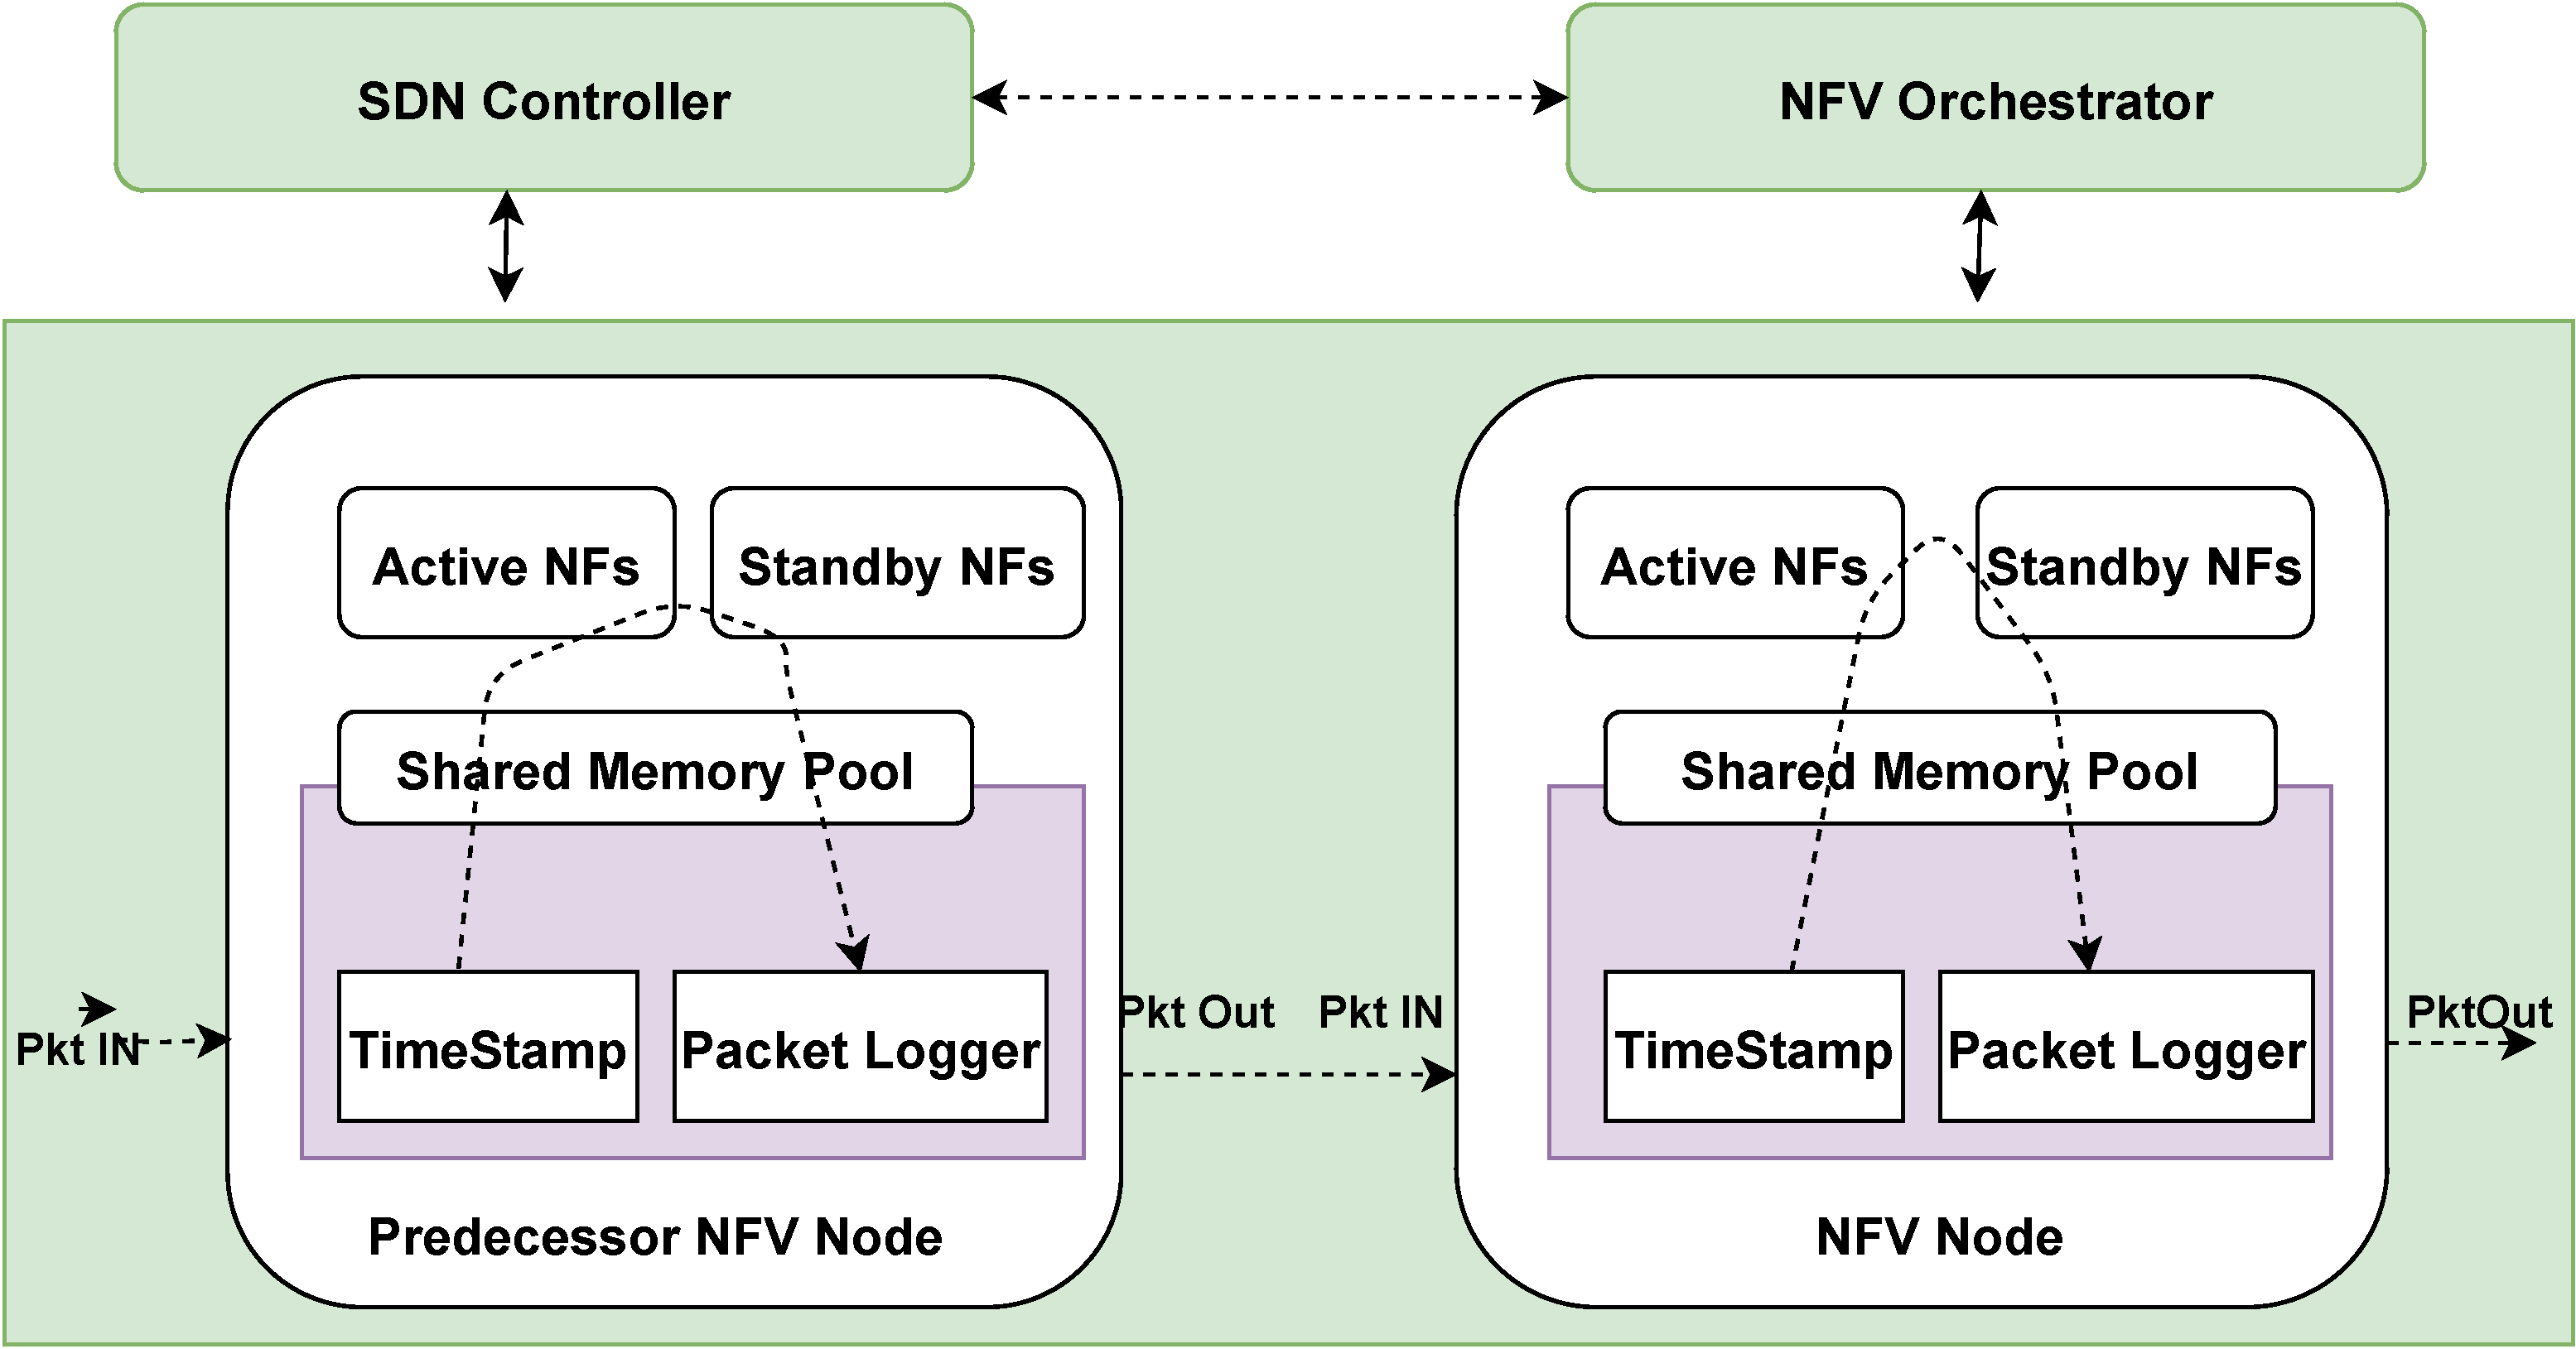
\includegraphics[width=0.9\columnwidth]{REINFORCE.pdf}
\caption{REINFORCE framework.}
\label{REINFORCE}
\end{figure}



%%%%%%%%%%%%%%%%%%%%%%%%%%%%%%%%%%%%%%%%%%%
\subsubsection{{Hmaity et al.}}%please check  if the title is correct.
\label{SFC-failures}
Hmaity {et al.}~\cite{hmaity2016virtual} presented a solution that  uses integer linear programming to solve the problem of link and node failures in service chains. They modelled the physical infrastructure using a directed network graph, with representations for physical devices with the ability to host virtual network functions and links. The latencies of physical links and packet processing latency by vNFs are also represented in the model of the physical network topology. The other components that were modelled are the service chains and the vNFs, which are considered as abstract components that can process ingress packets before forwarding to the next vNF or host device.

The constraints considered for the proposed model are (i) node capacity and link latency, which capture the current state of a node, the capacity of the link in use, the latency and the highest number of virtual machines that can be hosted by a particular node; (ii)~constraints related to routing, such as the location of virtual links in the physical network, to ensure that routing paths are made available on the right physical node; and (iii) constraints related to the placement of vNFs on physical devices, by ensuring that active and standby vNFs are not collocated on the same node.

The proposed models were evaluated using two example service chains, that is, a chain consisting of a web service and another service chain that models online gaming, where the impacts on node capacity and latency were considered. To solve the formulated ILP model, a bandwidth of 100 kbit/s was set for the online gaming service chain, while 50 kbit/s was set for the web service scenario. Latencies of 500 ms and 60 ms were set for the service chains. The proposed and solved models showed that achieving SFC resilience requires additional (redundant) nodes of approximately 107\%. Although the proposed solution serves as a good mechanism that can handle link and node failures in service chains, it lacks the ability to provide shared protection against failures.    


%%%%%%%%%%%%%%%%%%%%%%%%%%%%%%%%%%%%%%%%%%%%%
\subsubsection{Resilient SFCs---Medhat et al.}
\label{Medhat et al.}

Medhat {et al.}~\cite{medhat2016resilient} proposed an OpenStack and OpenDaylight-based environment to deploy and orchestrate resilient SFCs in cloud environments. The proposed framework follows the ETSI NFV model, which is capable of traffic rerouting, in the case of faults occurring at runtime. The authors proposed an extension to the ETSI NFV framework for SFC orchestration and management, with the implementation of a service chain consisting of two firewall network functions in standby and active modes. 

They  used the Open Baton framework~\cite{carella2015open} as the NFVO, which uses a messaging queue to communicate with the SFC orchestrator (the OpenDaylight SDN Controller), and the Zabbix network monitoring tool. Service function failure is simulated by abruptly terminating the process running the NF, then the Open Baton Fault Management System (FMS) switches to the standby network function, and the failed NF is recovered by the~Orchestrator.


%%%%%%%%%%%%%%%%%%%%%%%%%%%%%%%%%%%%%%%%%%%%%%%%%%
\subsubsection{OpenFlow Fault Recovery}
\label{OpenFlow-Fault}
The framework proposed by Nguyen {et al.}~\cite{nguyen2019openflow} used the OpenFlow group table to provide a quick fault recovery and fast fail-over scheme. Their proposal eliminates the use of a centralised logical controller by exploiting the use of the OpenFlow group table for managing service function chains. Fault recovery and detection were implemented in local OpenFlow switches, which utilise an OF group table. 

The need to contact the controller or NFV-MANO in the event of a failure is eliminated, which saves time on fault notification and recovery. The framework was tested using OpenStack and OF, with two vFirewall functions deployed for redundancy, which showed a reduction in SFC packet loss and an improvement in link throughput, as well as quick failure recovery. 
We briefly explain the aspects of SFC resilience that require further attention from the research community in Section \ref{Resilience in SFC environments}. 





%%%%%%%%%%%%%%%%%%%%%%%%%%%%%%%%%%%%%%%%
%%%%%%%%%%%%%%%%%%%%%%%%%%%%%%%%%%%%%%%%
\section{State-of-the-Art and Open Challenges}
\label{Open-challenges}
The challenges that the classified frameworks in Section \ref{SFC implementation frameworks} try to solve and the approach used are presented in Tables   \ref{Resource-Allocation-Table}--\ref{Resilience Table}. This captures the proposed solutions, the packet processing element(s) used, and the test bed or proof of concept employed by the authors. In this section, we present some key aspects of SFC implementations, where we focus on the open challenges (depicted in Figure \ref{OpenChallenges-pic}) and highlight some of the existing efforts to solve the problems presented.


\begin{figure}[H]%[H]
%\centering
%\includegraphics[width=0.8\textwidth]{PhantomSFC.png}
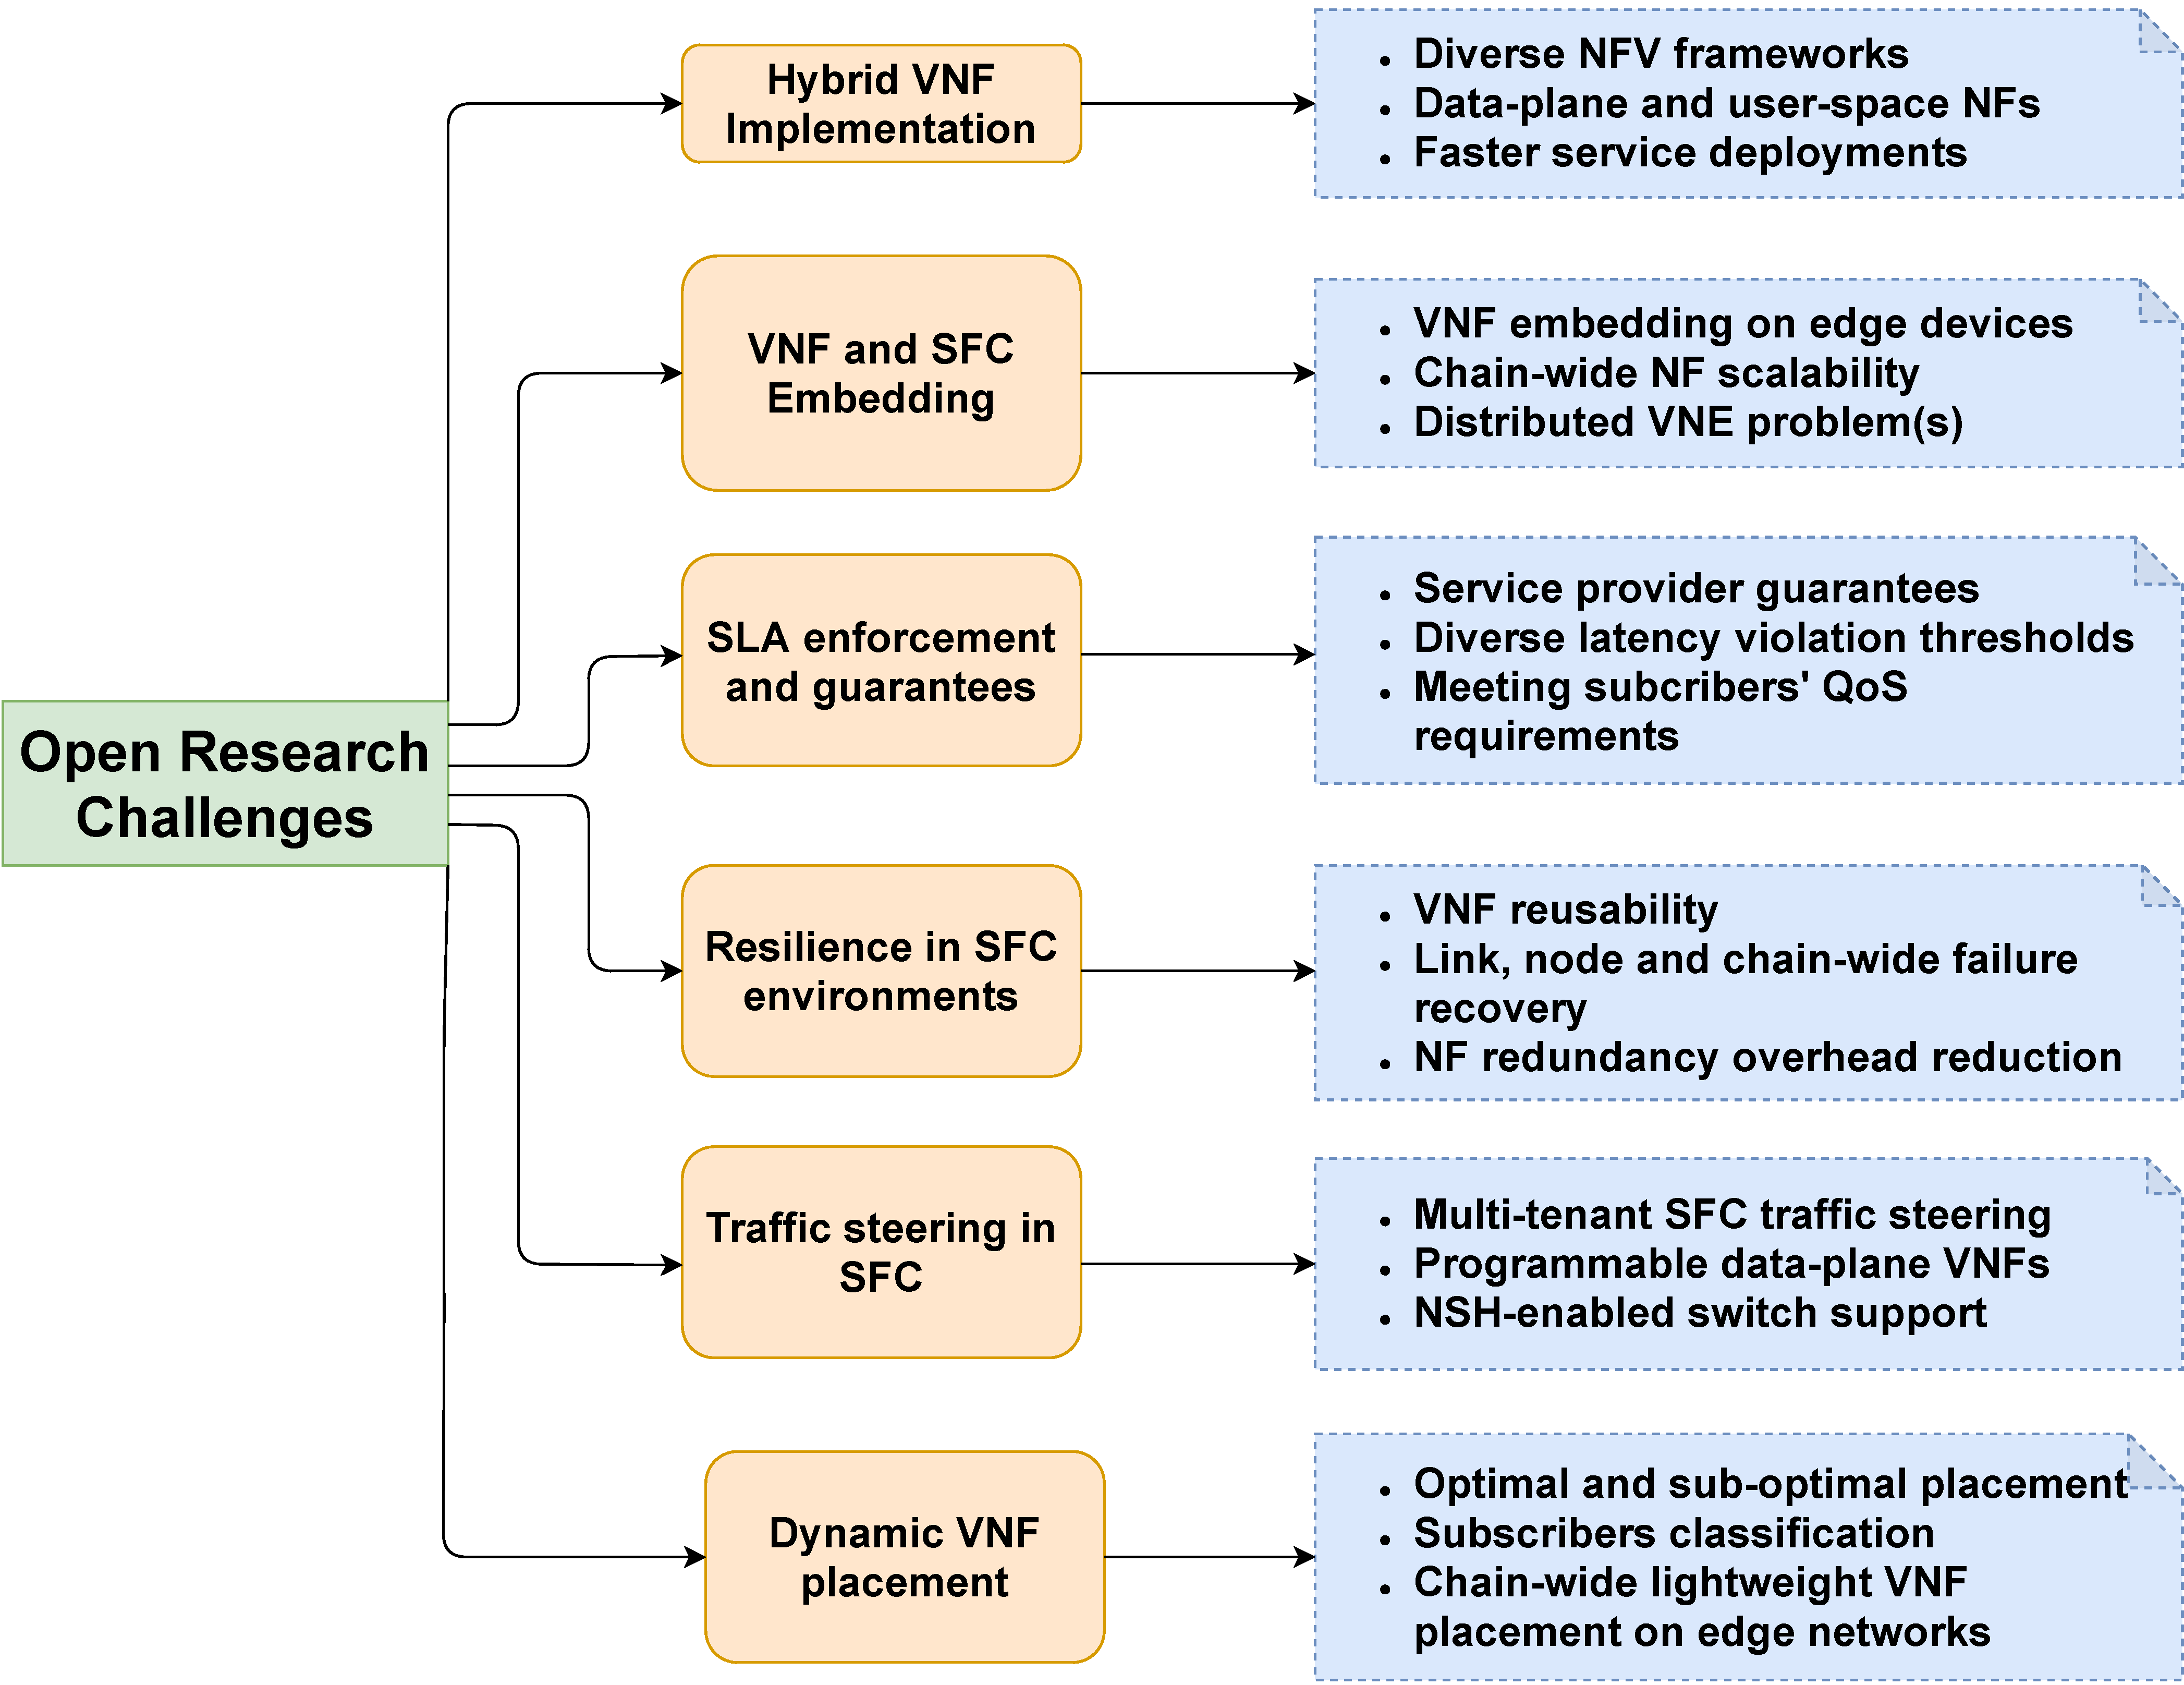
\includegraphics[width=0.9\columnwidth]{OpenChallenges.pdf}
\caption{State-of-the-art and open research challenges.}
\label{OpenChallenges-pic}
\end{figure}


%%%%%%%%%%%%%%%%%%%%%%%%%%%%%%%%

%%%%%%%%%%%%%%%%%%%%%%%%%%%%%%%%

%%%%%%%%%%%%%%%%%%%%%%%%%%%%%%%%%%%%%%%%%
\subsection{Hybrid vNF Implementation}
\label{Hybrid}
There are diverse frameworks for implementing virtual network functions in service provider network environments,  which can be used to implement network functions at the data plane of the network, using virtual switching technologies such as OpenvSwitch~\cite{jackson2016softflow} or P4~\cite{bosshart2014p4}. Virtual network functions can also be implemented in the user space, using unikernels~\cite{kurek2019unikernel}, virtual machines~\cite{laghrissi2017towards}, GPUs~\cite{yi2017gpunfv}, or containers~\cite{zhang2016opennetvm}. 

Because NFV and SDN allow for the creation of chains of network functions for efficient packet processing, it is ideal to create a processing pipeline that supports fast service delivery and efficient use of available resources by service providers to support future networks. Creating a service function chain (SFC) currently involves the chaining of network functions that are either implemented at the data plane or as user-space functions and are often carried out using network functions that are built using the same framework to create processing elements. The current data-plane technology does not easily provide support for operations such as the manipulation of floating-point values~\cite{simpson2020seidhr} or security~modules. 

Thus, the resource-constrained nature of the data plane also poses some limitations in terms of implementing resource-hungry network functions. We question the way in which network functions are currently implemented (including the composition of the network functions that create a service chain) and seek to argue for a hybrid implementation approach that combines user-space and data-plane components to create a chain of network functions along the processing pipeline. 

It is correct to state that diverse frameworks have their constraints and benefits, and a hybrid implementation framework will leverage the benefits of both user space and data plane by composing processing pipelines using diverse frameworks. A hybrid NF implementation framework combines the available resources in the user space and the fast processing speed of the network data plane, with the aim of reducing end-to-end latency and improving packet throughput and CPU utilisation.

Van {et al.}~\cite{van2019building} proposed a hybrid NFV framework for building low-latency and high-throughput vNFs using XDP. Simple operations are handled by the XDP program, whereas complex operations are handled by a user-space program. Three example NFs were chained (with two SFCs) using OpenStack. The performance of the framework was measured using throughput, latency, and CPU utilisation. They also considered the performance of the DPDK when interconnecting multiple vNFs. Their framework separates packet processing into fast and slow paths, with less complex NFs (simple LB and flow statistics) handled by the slow path, whereas vNFs that require complex processing are handled by the fast path.  A use case example is a load balancer, which can be implemented in XDP if it uses a simple hash algorithm and is implemented using the hybrid approach if the NF is sophisticated. 

Van et al.~\cite{van2017architecture}  used an extended Berkeley packet filter (eBPF), which is a Linux kernel framework that provides flexible kernel-level manipulation of packet processing pipelines. Their proposal was designed with the goal of having simple tasks handled by the kernel and complex NFs implemented in the user space. Two vNFs were built to test the proposed architecture: a dynamic traffic load balancer and a DPI network function. Compared to OpenFlow, the kernel-user interaction time is reduced with eBPF, which also provides better programmability options at the data plane.  

Efforts such as HYPER~\cite{sun2017hyper} focus on creating a hybrid NFV framework that can leverage softwarized network functions and implementations on hardware devices, without  considering whether the network functions are deployed at the network data plane or in the user space. Marcuzzo {et al.}~\cite{marcuzzo2020enabling} proposed a framework for offloading parts of a virtual network function to a programmable data plane. 

The proposed architecture can offload specified components of a network function, and at the same time provide support in situations where NF offloading is not desirable. The management component of the framework comprises: (1) an interface for service providers (the user module), which can be used by users to initiate or stop an offload request; (2) a module for translating offload code that has been compiled for installation on data-plane programmable devices, (3) a module that serves as the offload manager, for handling compiled offload code and communication with the NFV component; and (4)~NFV and SDN modules for handling connections to the controller, topological data, and flow rule installation (SDN module), while communication with the offload agents on the network functions is handled by the NFV module.

Although the proposal presented by Marcuzzo {et al.}~\cite{marcuzzo2020enabling} aims to push some components of network functions down to the data plane of the network, it is not entirely a hybrid framework that composes packet processing pipelines from diverse NFV frameworks. Similarly,~refs.~\cite{sun2017hyper,van2017architecture,van2019building} attempted to solve the problem of data plane and user-space packet processing using network functions built from the same framework(s).



%%%%%%%%%%%%%%%%%%%%%%%%%%%%%%%%%%%%%
\subsection{vNF and SFC Embedding}
\label{VNF Embedding}
Embedding virtual network functions on physical infrastructure is at the core of the creation of service function chains in service provider networks. Different authors have proposed solutions to solve the problems of vNF and SFC embedding. Reddy {et al.}~\cite{reddy2016robust} on embedding vNFs employed a mixed-integer linear programming (MILP) model, which handles the problem as a resource optimisation problem, where the scalability of the proposed model was enhanced using a variable neighbourhood search heuristic. 

Pei {et al.} considered the embedding of SFCs in distributed cloud environments, with the aim of embedding service requests by reducing overheads. They approached the service chain embedding problem by formulating a binary integer programming (BIP) mechanism, which introduces algorithms aimed at the optimisation of the number of network functions that are placed along the service chain. 

The survey of heuristic solutions for solving the virtual network embedding (VNE) problem presented by Cao {et al.}~\cite{cao2018heuristic} captures some recent efforts that focus on embedding virtual network functions on substrate networks. Their work categorised heuristic algorithms for solving the VNE problem into (1) dynamic or static, (2) distributed or centralised, and (3) redundant or concise. Static VNE algorithms require less computation than dynamic solutions, which depends on the complexity of the substrate network and the virtual network function in use. 

In their work, Sun 
{et al.}~\cite{sun2020energy} proposed an energy-aware routing and adaptive delayed shutdown (EAR-ADS) model that supports the deployment of SFCs in a dynamic manner. Their proposed solution considers a practical scenario where overall deployment cost is minimized as well as balanced energy consumption by servers. Shutdown delays of servers are also reduced, which minimizes the effect of energy fluctuations associated with most network environments. The results presented show a huge reduction in energy costs and the overall stability of the network also improves.

The ability to dynamically reconfigure the embedded network functions makes the dynamic VNE algorithm ideal for next-generation networks~\cite{li2021multi}. Unlike the distributed VNE problem, the centralised problem makes use of a single-substrate infrastructure for embedding virtual network functions in future network environments. Computation in the distributed VNE algorithm is carried out by two or more substrate networks, which leads to improved scalability and the elimination of a single point of failure. Concise VNE heuristic algorithms are concerned with the exact number of substrate networks that are required to meet the SLA involved in embedding the virtual networks. The disadvantage of this approach is the lack of a guarantee for failure recovery. Redundant VNE solutions provide a provision for failure recovery by reserving the substrate network resources.   

We believe that this remains an open challenge for the research community. Next-generation networks are generally envisaged to be completely softwarized, which should make the deployment of network functions doable at the network edge, which is closer to the point of traffic generation. The creation of chains of network functions is also seen as one of the major aspects of next-generation networks, which raises the question of embedding network functions on multiple commodity servers or embedding all functions on a single physical server for the creation of service chains. Questions such as the scalability of such functions in the chain and the dynamic embedding of network functions, based on application profiles and QoS requirements, still need to be addressed.



%%%%%%%%%%%%%%%%%%%%%%%%%%%%%%%%%%%%%%%%%%%%%%%
\subsection{SLA Enforcement and Guarantees}
\label{SLA enforcement and guarantees}
There is very little work currently in the literature that considers the enforcement of policies and SLAs by service providers, which revolves around finding out what service providers can guarantee in a NFV/SFC environment. Based on the recent literature, we argue that being able to adapt the QoS to frequent network changes is still a challenge in SFC environments for next-generation networks, and the ability to assess and visualise QoS requirements and parameters~\cite{zhao2021security} will help in satisfying the long-term vision of SFC~deployments. 

Wang {et al.}~\cite{wang2018improving} presented a QoE-driven service chain deployment, which also provides latency prediction features. Their focus was on improving the overall QoE for the user by reducing the number of rejections and waiting time experienced by users when accessing services. According to Herbaut {et al.}~\cite{herbaut2016deploying}, Content Delivery Network (CDN) providers can negotiate the SLA with the vNF provider by requesting the creation of virtual CDN (vCDN) instances. An example is a CDN providing video streaming services such as YouTube or NetFlix. The focus of the SLA agreement between the CDN and the vNF provider in this scenario will be on the bandwidth and delay requirements of the service that is being~provided. 

Sun {et al.}~\cite{sun2016sla} proposed SLA-NFV, which is an SLA-aware framework  that focuses on the SLAs of the tenants (service subscribers). Their framework leverages a hybrid infrastructure, programmable hardware, and software, with the goal of enhancing the capability of NFV in handling different SLAs. The experimental results show that SLA-NFV, which creates a hybrid NFV, reduces latency by approximately 60\% when compared to a software service chain. Their work did not consider a solution that helps service providers  meet the diverse SLA requirements needed for the operation of next-generation~networks. 


%%%%%%%%%%%%%%%%%%%%%%%%%%%%%%%%%%%%%%%%%%%%%%%%%
\subsection{Resilience in SFC Environments}
\label{Resilience in SFC environments}

Although our work considered efforts in the literature that try to solve the problem of resilience in NFV and SFC, resilience and fault tolerance are still major concerns in SFC environments, especially where the focus is on vNF reusability~\cite{chowdhury2019re}. Achieving cost-effective resilience is still an open challenge in SFC implementation frameworks, and there are unanswered questions for future research which include how SFCs respond to failure conditions such as links between SFFs. The failure of the virtual network functions themselves is an aspect that needs to be considered as a long term vision that requires further research, that is, with the consideration of having redundant SFs along the SFP to handle failure scenarios.

Synthesising network processing graphs or service chains is another approach that is employed to achieve high availability in SFC, as well as the use of a multi-path routing approach~\cite{cai2021disaster}. As indicated by Mirjalily {et al.}~\cite{mirjalily2018optimal}, simple approaches such as the use of traffic load balancers can help with dynamic re-routing of traffic to alternate processing pipelines in SFC environments. However, an efficient load-balancing algorithm that tracks device states and available resources needs to be implemented, which goes beyond the basic round-robin algorithm that is commonly deployed in today's network environments.

Approaches such as the work by Ghaznavi {et al.}~\cite{ghaznavi2020fault} try to provide SFC resilience and at the same time eliminate the need for NF replication, in order to reduce overhead. This is achieved by collecting and piggybacking NF state changes as packets traverse the service chain; thus, the overhead is reduced because the entire network function is not replicated to a standby node. A key challenge with proposals that employ the use of service replication is the amount of overhead incurred with redundant backup links, nodes, and service chains; thus, the efficient implementation of a high-availability failure mechanism is still a research challenge that requires further attention.  


%%%%%%%%%%%%%%%%%%%%%%%%%%%%%%%%%%%%%%%%%%%%%%
\subsection{Traffic Steering in SFC} 
\label{Traffic steering in SFC}
From the related literature on SFC traffic steering, we believe that the ability to dynamically steer traffic to the edge of the network, which adapts to network changes, is still required and desirable for the operation of next-generation networks. We also argue that having a functional programmable data-plane, which is a core component of future networks, can solve the problem of always having to install flow rules on virtual switches to steer traffic. 

The ability to obtain the current network state and dynamically update the current service function path in real time requires more work to achieve better traffic steering in SFC for next-generation networks. Other factors such as delivery time, measuring virtual machines’ (along the service path) usage, latency, and delay~\cite{nemeth2021delay}, are some of the considerations still open for further research with respect to service path selection in SFCs. 

Our review of some related literature on SFC traffic steering also shows that the inter-operability between traffic steering techniques is still a challenge, as different service providers employ traffic steering approaches that best meet their business requirements. Multi-tenant networks also require a scalable traffic-steering scheme for SFC, as future networks are envisaged to be more heterogeneous in nature~\cite{bouridah2021optimized}. As it relates to steering traffic in SFC environments, service functions need to have support for SFC encapsulation protocols and headers.

Traffic steering types can be classified into three categories: header-based methods, tag-based methods, and programmable switch-based methods, which deal with the re-classification of flows and network isolation, where traffic forwarding depends on the configurations sent from the SDN controller to the switches. Tag-based steering methods make use of MAC addresses, VLANs, and MPLS tags to steer incoming traffic. Header-based methods  use the network service header (NSH), service chain header (SCH), IP option field, and segmented routing header~\cite{hantouti2018traffic}. 

Medhat {et al.}~\cite{medhat2016service} identified the absence of network service header (NSH) capability in switches as one of the challenges with traffic steering in SFC environments. Some proposals include the use of MAC addresses and tags to steer traffic in a service chain. Having virtual switches, such as Open vSwitch (OvS), which supports NSH capability, would allow for better traffic tagging and steering.  




%%%%%%%%%%%%%%%%%%%%%%%%%%%%%%%%%%%%%%%%%%%%
\subsection{Dynamic vNF Placement}
\label{vNF placement}
Most of the current approaches used in vNF placement, presented in Section \ref{SFC implementation frameworks}, create a scenario in which all users contribute to a single latency violation threshold, which is common to all users. In line with the long term vision of next generation networks, an improved approach will help providers with different groups of applications such as VoIP/telephony users with a latency violation threshold, which should be lower than the threshold assigned to other classes of applications with less sensitive requirements in terms of latency. One justification that supports this argument is the much-anticipated rise in the number of end users with unique service requirements~\cite{wang2021availability}, which will affect the way in which vNFs are deployed in the future.. 

The placement of virtual Network Functions (vNFs) affects the latency between users and the vNFs, and thus we believe that a better placement design needs to be implemented for future networks, which prioritises the reduction in the negative effects of performance change, caused by the “hop-by-hop” movement of users between different vNFs. We argue that the cost implications of placing service functions in the SFC still need to be addressed, which is one of the open challenges in this domain. Other related challenges include creating placement schemes that  consider parameters such as subscriber preferences, infrastructure properties, and delivery time. 

Bhamare {et al.}~\cite{bhamare2018exploring} presented a novel fair weighted scheduling (FWS) solution for the scheduling of microservices in multi-cloud environments for the optimal creation of service function chains. Their proposed solution considers delays and SLA-related costs in deploying service function chains. They were able to reduce the overall turnaround time while considering the total network delays and variable loads. The solution was compared to the standard biased greedy approach, which showed a notable increase in performance. The authors acknowledge the need for further investigations into microservices-related challenges such as security, fault tolerance, load balancing, and distributed data management.

Chai {et al.}~\cite{chai2019parallel} proposed a parallel placement scheme, PP-DRL, which uses deep reinforcement learning (DRL) to deploy SFCs optimally with minimal resource costs. They also  used DRL to determine the right servers that could host service functions by collecting the characteristics of user requests as state information. They first used DRL to calculate the number of virtual machines and to find servers that can be used for hosting vNFs. The location of the end users is not prioritised in the scheme.

In their work, Laghrissi {et al.}~\cite{laghrissi2017towards} presented an efficient tool, which they called the “Network Slice Planner”, for spatio-temporal simulation of mobile service usage, to maximise QoS for the users. They modified the classic predictive algorithm after presenting a set of existing placement algorithms. The performance of the enhanced predictive algorithm was compared with existing vNF placement algorithms, which showed slightly better results. Although they modelled the behaviour of the end users (in terms of traffic types), their proposed solution does not prioritise the placement of vNFs at the edge of the~network. 

Bhamare {et al.}~\cite{bhamare2017optimal} explain how the optimal placement of vNFs across multiple clouds is a problem which, when solved, can help in the optimization of parameters such as cost, network delay, and bandwidth. After presenting the components of an SFC environment, they presented an analytical model for the placement of service functions in multi-cloud network environments. Their work  considers delays to end-users, QoS, and SLA. They employed an ILP approach to obtain the optimal solution,  which was achieved by setting up an objective function and applicable constraints. 

Cziva {et al.}~\cite{cziva2018dynamic} considered the placement of vNFs in a distributed-edge NFV environment with dynamic orchestration and re-calculation of vNF placement. They formulated and solved the edge vNF placement problem using the fundamentals of the optimal stopping theory (OST). They presented a time-optimized scheduler for optimal placement of vNFs at the edge of the network, and considered an undirected network graph comprising hosts, links between hosts, and users on the network. An assumption was made by the authors that resources on the hosts are finite and that links have a physical limit when it comes to bandwidth along the path. 



%%%%%%%%%%%%%%%%%%%%%%%%%%%%%%%%%%%%%%%%%%%%%%
%%%%%%%%%%%%%%%%%%%%%%%%%%%%%%%%%%%%%%%%%%%%%%
\section{Conclusions}
\label{Conclusion}

The concept of service function chaining evolves as service providers continue to explore the benefits of deploying streamlined services for end users. Several approaches have been proposed in the literature for deploying network function virtualisation and solving different problems that involve chaining such network functions to meet user~requirements.

In this work, we presented NFV environments and the requirements for chaining network functions for effective service delivery.

We conducted a comprehensive survey focusing on the NFV frameworks that also support the chaining of virtual network functions. We created a taxonomy of SFC implementation frameworks, a classification of the problems they attempted to solve, and discussed the open research challenges in SFC environments. The taxonomy presented separates the frameworks into three main categories: resource allocation and service orchestration, performance tuning, resilience, and fault recovery.

Important challenges that require further attention from the research community include the implementation of a hybrid NFV framework which can leverage processing resources from heterogeneous environments, including the orchestration of diverse vNFs. Other open challenges that should be addressed to support future networks are the optimisation of dynamic traffic steering in SFC, the efficient placement of heterogeneous network functions from diverse vendors, meeting SLA guarantees by service providers, and vNF/SFC embedding on commodity servers. 
All the open research challenges we have presented describe the problem, the importance of addressing each problem, explain the subcomponents of the problem (also depicted in Figure \ref{OpenChallenges-pic}), how each of the identified problems relate to the operation of next generation networks, and discuss prominent attempts to tackling them. Our work provides researchers in the NFV/SFC domain a clear picture of what has been achieved so far and the areas that require further research in order for the long term vision of service function chaining to be achieved.  
%%%%%%%%%%%%%%%%%%%%%%%%%%%%%%%%%%%%%%%%%%
\vspace{6pt} 
%%%%%%%%%%%%%%%%%%%%%%%%%%%%%%%%%%%%%%%%%%
%% optional
%\supplementary{The following are available online at \linksupplementary{s1}, Figure S1: title, Table S1: title, Video S1: title.}

% Only for the journal Methods and Protocols:
% If you wish to submit a video article, please do so with any other supplementary material.
% \supplementary{The following are available at \linksupplementary{s1}, Figure S1: title, Table S1: title, Video S1: title. A supporting video article is available at doi: link.} 

%%%%%%%%%%%%%%%%%%%%%%%%%%%%%%%%%%%%%%%%%%
\authorcontributions{Conceptualization, H.U.A. and D.P. P.; Methodology, H.U.A. and D.P. P.;
Resources, H.U.A. and D.P. P.; Writing—original draft preparation, H.U.A. and D.P. P.; Writing—
review and editing, H.U.A. and D.P.P.;  Supervision, D.P.P.  All authors have read and agreed to this draft of the manuscript.}

\funding{{This  work  was  supported  in  part  by  the  UK  Engineering and  Physical  Sciences  Research  Council  (EPSRC)  grant EP/N033957/1, the PETRAS National Centre of Excellence for IoT Systems Cybersecurity, which has been funded by the UK EPSRC under grant number EP/S035362/1 and the Petroleum Technology Development Fund (PTDF) Nigeria, grant 1563/19.}}%Funding same as Acknowledgments, please revise.

\institutionalreview{Not applicable.}

\informedconsent{Not applicable.}

\dataavailability{Not applicable.} 

%\acknowledgments{{This  work  was  supported  in  part  by  the  UK  Engineering and  Physical  Sciences  Research  Council  (EPSRC)  grant EP/N033957/1, the PETRAS National Centre of Excellence for IoT Systems Cybersecurity, which has been funded by the UK EPSRC under grant number EP/S035362/1 and the Petroleum Technology Development Fund (PTDF) Nigeria, grant 1563/19.}}
\conflictsofinterest{No conflict of interest.} 


\abbreviations{Abbreviations}{%
{The} %MDPI: Please consider this suggested change.
 following abbreviations are used in this manuscript:\\

%%%%%%%%%%%%%%%%%%%%%%%%%%%%%%
%\begin{table}[H]
%\caption{List of abbreviations}
%\begin{center}

\noindent
\begin{tabular}{@{}m{2cm}<{\raggedright}m{10cm}<{\raggedright}}
%\toprule
{\textbf{Abbreviation}} & {\textbf{Meaning}}\\
%\midrule
%SFC & \makecel{Service Function Chaining}\\
API & Application programming interface \\

CAPEX & Capital expenditure \\

CL & Classifier \\

CNF & Cloud-native function \\

DMA & Direct memory access \\

DPI & Deep packet inspection \\

eNF & embedded network function \\

ETSI & European Telecommunication Standards Institute \\

FPGA & Field-programmable gate array \\

EPC & Evolved packet core \\



ITU & International telecommunication union \\

IDS & Intrusion detection system \\

ILP & Integer linear programming \\

IoT & Internet of Things \\

IPS & Intrusion prevention system \\

PCAP & Packet capture\\

PoC & Proof of concept \\

RSS & Receive side scaling \\

SC & Service Chain \\


SDN & Software-defined networking \\

SFF & Service function forwarder \\

SP & Service provider \\\end{tabular}

\noindent
\begin{tabular}{@{}m{2cm}<{\raggedright}m{10cm}<{\raggedright}}

SF & Service function \\

SFCC & Service function chaining controller \\

MAC & Media access control \\

ML & Machine learning \\

NAT & Network address translation \\

NFV & Network function virtualization\\

NSH & Network service header \\

NFVI & NFV infrastructure \\

NFVO & NFV Orchestrator \\

NS & Network service \\

NFF & Network function forwarder \\

OF & OpenFlow \\

OPEX & Operational expenditure \\

QoS & Quality of service \\

QoE & Quality of experience \\

vCPE & virtual customer premises equipment \\

VNE & Virtual network embedding \\

VoIP & Voice over Internet Protocol \\

vNF & Virtual network function \\

VNFC & Virtual network function component \\

SFC & Service function chaining \\

VIM & Virtual infrastructure manager \\
%\bottomrule
\end{tabular}
%\label{Abbreviations}
%\end{center}
%\end{table}
}
%\noindent 





\begin{adjustwidth}{-\extralength}{0cm}
%\printendnotes[custom] % Un-comment to print a list of endnotes

\reftitle{References}

%%%REFS
%%%%%%%%%%%%%%%%%%%%%%%%%%%%%%%%%%%%%%%%%%
\begin{thebibliography}{999}

\bibitem[Herrera and Botero(2016)]{herrera2016resource}
Herrera, J.G.; Botero, J.F.
\newblock Resource allocation in NFV: A comprehensive survey.
\newblock {\em IEEE Trans. Netw. Serv. Manag.} {\bf 2016},
  {\em 13},~518--532.

\bibitem[Cherrared \em{et~al.}(2019)Cherrared, Imadali, Fabre, G{\"o}ssler, and
  Yahia]{cherrared2019survey}
Cherrared, S.; Imadali, S.; Fabre, E.; G{\"o}ssler, G.; Yahia, I.G.B.
\newblock A survey of fault management in network virtualization environments:
  Challenges and solutions.
\newblock {\em IEEE Trans. Netw. Serv. Manag.} {\bf 2019},
  {\em 16},~1537--1551.

\bibitem[Paganelli \em{et~al.}(2021)Paganelli, Cappanera, and
  Cuffaro]{paganelli2021tenant}
Paganelli, F.; Cappanera, P.; Cuffaro, G.
\newblock Tenant-defined service function chaining in a multi-site network
  slice.
\newblock {\em Future Gener. Comput. Syst.} {\bf 2021}, {\em
  121},~1--18.

\bibitem[Laghrissi and Taleb(2018)]{laghrissi2018survey}
Laghrissi, A.; Taleb, T.
\newblock A survey on the placement of virtual resources and virtual network
  functions.
\newblock {\em IEEE Commun. Surv. Tutor.} {\bf 2018}, {\em
  21},~1409--1434.

\bibitem[Bujari \em{et~al.}(2019)Bujari, Palazzi, Polonio, and
  Zanella]{bujari2019service}
Bujari, A.; Palazzi, C.E.; Polonio, D.; Zanella, M.
\newblock Service function chaining: A lightweight container-based management
  and orchestration plane.
\newblock  {In Proceedings of the} 
2019 16th IEEE Annual Consumer Communications \& Networking
  Conference (CCNC),  Las Vegas, NV, USA, 11--14 January 2019; pp. 1--4.

\bibitem[Santos \em{et~al.}(2020)Santos, Wauters, Volckaert, and
  De~Turck]{santos2020towards}
Santos, J.; Wauters, T.; Volckaert, B.; De~Turck, F.
\newblock Towards delay-aware container-based service function chaining in fog
  computing.
\newblock  {In Proceedings of the} NOMS 2020-2020 IEEE/IFIP Network Operations and Management  %please add location and date of meeting, There are more than 30 places that need to be added.
  Symposium,  Budapest, Hungary, 20--24 April 2020; pp. 1--9.

\bibitem[Li and Qian(2016)]{li2016survey}
Li, X.; Qian, C.
\newblock A survey of network function placement.
\newblock  {In Proceedings of the} 2016 13th IEEE Annual Consumer Communications \& Networking
  Conference (CCNC),  Las Vegas, NV, USA,  9--12 January 2016; pp. 948--953.

\bibitem[Haleplidis \em{et~al.}(2014)Haleplidis, Joachimpillai, Salim, Lopez,
  Martin, Pentikousis, Denazis, and Koufopavlou]{haleplidis2014forces}
Haleplidis, E.; Joachimpillai, D.; Salim, J.H.; Lopez, D.; Martin, J.;
  Pentikousis, K.; Denazis, S.; Koufopavlou, O.
\newblock ForCES applicability to SDN-enhanced NFV.
\newblock  {In Proceedings of the} 2014 Third European Workshop on Software Defined Networks,  Budapest, Hungary, 1--3 September 2014; pp. 43--48.

\bibitem[Liu \em{et~al.}(2017)Liu, Lu, Zhou, Lu, and Zhu]{liu2017dynamic}
Liu, J.; Lu, W.; Zhou, F.; Lu, P.; Zhu, Z.
\newblock On dynamic service function chain deployment and readjustment.
\newblock {\em IEEE Trans. Netw. Serv. Manag.} {\bf 2017},
  {\em 14},~543--553.

\bibitem[Chua \em{et~al.}(2016)Chua, Ward, Zhang, Sharma, and
  Huberman]{chua2016stringer}
Chua, F.C.; Ward, J.; Zhang, Y.; Sharma, P.; Huberman, B.A.
\newblock Stringer: Balancing latency and resource usage in service function
  chain provisioning.
\newblock {\em IEEE Internet Comput.} {\bf 2016}, {\em 20},~22--31.

\bibitem[Bhamare \em{et~al.}(2017)Bhamare, Samaka, Erbad, Jain, Gupta, and
  Chan]{bhamare2017optimal}
Bhamare, D.; Samaka, M.; Erbad, A.; Jain, R.; Gupta, L.; Chan, H.A.
\newblock Optimal virtual network function placement in multi-cloud service
  function chaining architecture.
\newblock {\em Comput. Commun.} {\bf 2017}, {\em 102},~1--16.

\bibitem[Martins \em{et~al.}(2014)Martins, Ahmed, Raiciu, Olteanu, Honda,
  Bifulco, and Huici]{martins2014clickos}
Martins, J.; Ahmed, M.; Raiciu, C.; Olteanu, V.; Honda, M.; Bifulco, R.; Huici,
  F.
\newblock ClickOS and the art of network function virtualization.
\newblock  {In Proceedings of the} 11th USENIX Symposium on Networked Systems Design and
  Implementation (NSDI 14),  Seattle, WA, USA, 2--4 April 2014; pp. 459--473.

\bibitem[Zhang \em{et~al.}(2016)Zhang, Liu, Zhang, Shah, Lopreiato, Todeschi,
  Ramakrishnan, and Wood]{zhang2016opennetvm}
Zhang, W.; Liu, G.; Zhang, W.; Shah, N.; Lopreiato, P.; Todeschi, G.;
  Ramakrishnan, K.; Wood, T.
\newblock OpenNetVM: A platform for high performance network service chains.
\newblock  {In Proceedings of the} 2016 Workshop on Hot topics in Middleboxes and
  Network Function Virtualization,  Florianopolis, Brazil, 22 August 2016; pp. 26--31.

\bibitem[Bremler-Barr \em{et~al.}(2016)Bremler-Barr, Harchol, and
  Hay]{bremler2016openbox}
Bremler-Barr, A.; Harchol, Y.; Hay, D.
\newblock OpenBox: A software-defined framework for developing, deploying, and
  managing network functions.
\newblock  {In Proceedings of the} 2016 ACM SIGCOMM Conference,  Florianopolis, Brazil, 22 August 2016; pp. 511--524.

\bibitem[Anwer \em{et~al.}(2015)Anwer, Benson, Feamster, and
  Levin]{anwer2015programming}
Anwer, B.; Benson, T.; Feamster, N.; Levin, D.
\newblock Programming slick network functions.
\newblock  {In Proceedings of the} 1st ACM Sigcomm Symposium on Software Defined
  Networking Research,  Santa Clara, CA, USA, 17 June 2015; pp. 1--13.

\bibitem[Katsikas \em{et~al.}(2016)Katsikas, Enguehard, Ku{\'z}niar,
  Maguire~Jr, and Kosti{\'c}]{katsikas2016snf}
Katsikas, G.P.; Enguehard, M.; Ku{\'z}niar, M.; Maguire~Jr, G.Q.; Kosti{\'c},
  D.
\newblock SNF: Synthesizing high performance NFV service chains.
\newblock {\em PeerJ Comput. Sci.} {\bf 2016}, {\em 2},~e98.

\bibitem[Katsikas \em{et~al.}(2018)Katsikas, Barbette, Kostic, Steinert, and
  Maguire~Jr]{katsikas2018metron}
Katsikas, G.P.; Barbette, T.; Kostic, D.; Steinert, R.; Maguire, G.Q.,~Jr.
\newblock Metron: NFV Service Chains at the True Speed of the Underlying
  Hardware.
\newblock  {In Proceedings of the} 15th USENIX Symposium on Networked Systems Design and
  Implementation (NSDI 18),  Renton, WA, USA, 9--11 April 2018; pp. 171--186.

\bibitem[Panda \em{et~al.}(2016)Panda, Han, Jang, Walls, Ratnasamy, and
  Shenker]{panda2016netbricks}
Panda, A.; Han, S.; Jang, K.; Walls, M.; Ratnasamy, S.; Shenker, S.
\newblock NetBricks: Taking the V out of NFV.
\newblock {In Proceedings of the} 12th USENIX Symposium on Operating Systems Design and
  Implementation (OSDI 16),  Savannah, GA, USA, 2 November 2016; \mbox{pp. 203--216.}

\bibitem[Cziva \em{et~al.}(2015)Cziva, Jouet, White, and
  Pezaros]{cziva2015container}
Cziva, R.; Jouet, S.; White, K.J.; Pezaros, D.P.
\newblock Container-based network function virtualization for software-defined
  networks.
\newblock  {In Proceedings of the} 2015 IEEE Symposium on Computers and Communication (ISCC), Larnaca, Cyprus, 6--9 July  2015; \mbox{pp. 415--420.}

\bibitem[Zoure \em{et~al.}(2022)Zoure, Ahmed, and
  R{\'e}veill{\'e}re]{zoure2022network}
Zoure, M.; Ahmed, T.; R{\'e}veill{\'e}re, L.
\newblock Network Services Anomalies in NFV: Survey, Taxonomy, and Verification
  Methods.
\newblock {\em IEEE Trans. Netw. Serv. Manag.} {\bf 2022}, {doi:10.1109/TNSM.2022.3144582.} %MDPI: Newly added information, please confirm.


\bibitem[Zhang \em{et~al.}(2020)Zhang, Qiu, Linguaglossa, Cerroni, and
  Giaccone]{zhang2020nfv}
Zhang, T.; Qiu, H.; Linguaglossa, L.; Cerroni, W.; Giaccone, P.
\newblock NFV platforms: Taxonomy, design choices and future challenges.
\newblock {\em IEEE Trans. Netw. Serv. Manag.} {\bf 2020},
  {\em 18},~30--48.

\bibitem[Hamdan \em{et~al.}(2021)Hamdan, Hassan, Abdelaziz, Elhigazi, Mohammed,
  Khan, Vasilakos, and Marsono]{hamdan2021comprehensive}
Hamdan, M.; Hassan, E.; Abdelaziz, A.; Elhigazi, A.; Mohammed, B.; Khan, S.;
  Vasilakos, A.V.; Marsono, M.N.
\newblock A comprehensive survey of load balancing techniques in
  software-defined network.
\newblock {\em J. Netw. Comput. Appl.} {\bf 2021}, {\em
  174},~102856.

\bibitem[Fei \em{et~al.}(2020)Fei, Liu, Zhang, Jin, and Hu]{fei2020paving}
Fei, X.; Liu, F.; Zhang, Q.; Jin, H.; Hu, H.
\newblock Paving the Way for NFV Acceleration: A Taxonomy, Survey and Future
  Directions.
\newblock {\em ACM Comput. Surv. (CSUR)} {\bf 2020}, {\em 53},~1--42.

\bibitem[Kaur \em{et~al.}(2020)Kaur, Mangat, and Kumar]{kaur2020comprehensive}
Kaur, K.; Mangat, V.; Kumar, K.
\newblock A comprehensive survey of service function chain provisioning
  approaches in SDN and NFV architecture.
\newblock {\em Comput. Sci. Rev.} {\bf 2020}, {\em 38},~100298.

\bibitem[Hantouti \em{et~al.}(2020)Hantouti, Benamar, and
  Taleb]{hantouti2020service}
Hantouti, H.; Benamar, N.; Taleb, T.
\newblock Service Function Chaining in 5G and Beyond Networks: Challenges and
  Open Research Issues.
\newblock {\em IEEE Netw.} {\bf 2020}, \emph{34}, 320--327.

\bibitem[Bonfim \em{et~al.}(2019)Bonfim, Dias, and
  Fernandes]{bonfim2019integrated}
Bonfim, M.S.; Dias, K.L.; Fernandes, S.F.
\newblock Integrated NFV/SDN architectures: A systematic literature review.
\newblock {\em ACM Comput. Surv. (CSUR)} {\bf 2019}, {\em 51},~1--39.

\bibitem[Hantouti \em{et~al.}(2018)Hantouti, Benamar, Taleb, and
  Laghrissi]{hantouti2018traffic}
Hantouti, H.; Benamar, N.; Taleb, T.; Laghrissi, A.
\newblock Traffic steering for service function chaining.
\newblock {\em IEEE Commun. Surv. Tutor.} {\bf 2018}, {\em
  21},~487--507.

\bibitem[Mirjalily and Zhiquan(2018)]{mirjalily2018optimal}
Mirjalily, G.; Zhiquan, L.
\newblock Optimal network function virtualization and service function
  chaining: A survey.
\newblock {\em Chin. J. Electron.} {\bf 2018}, {\em 27},~704--717.

\bibitem[Medhat \em{et~al.}(2016)Medhat, Taleb, Elmangoush, Carella, Covaci,
  and Magedanz]{medhat2016service}
Medhat, A.M.; Taleb, T.; Elmangoush, A.; Carella, G.A.; Covaci, S.; Magedanz,
  T.
\newblock Service function chaining in next generation networks: State of the
  art and research challenges.
\newblock {\em IEEE Commun. Mag.} {\bf 2016}, {\em 55},~216--223.

\bibitem[Bera \em{et~al.}(2017)Bera, Misra, and Vasilakos]{bera2017software}
Bera, S.; Misra, S.; Vasilakos, A.V.
\newblock Software-defined networking for internet of things: A survey.
\newblock {\em IEEE Internet Things J.} {\bf 2017}, {\em
  4},~1994--2008.

\bibitem[Veeraraghavan \em{et~al.}(2017)Veeraraghavan, Sato, Buchanan, Rahimi,
  Okamoto, and Yamanaka]{veeraraghavan2017network}
Veeraraghavan, M.; Sato, T.; Buchanan, M.; Rahimi, R.; Okamoto, S.; Yamanaka,
  N.
\newblock Network function virtualization: A survey.
\newblock {\em IEICE Trans. Commun.} {\bf 2017},  E100B,
  1978--1991. {https://doi.org/10.1587/transcom.2016NNI0001.} %MDPI: Newly added information, please confirm.


\bibitem[Bhamare \em{et~al.}(2016)Bhamare, Jain, Samaka, and
  Erbad]{bhamare2016survey}
Bhamare, D.; Jain, R.; Samaka, M.; Erbad, A.
\newblock A survey on service function chaining.
\newblock {\em J. Netw. Comput. Appl.} {\bf 2016}, {\em
  75},~138--155.

\bibitem[Xie \em{et~al.}(2016)Xie, Liu, Wang, and Wang]{xie2016service}
Xie, Y.; Liu, Z.; Wang, S.; Wang, Y.
\newblock Service function chaining resource allocation: A survey.
\newblock {\em arXiv} {\bf 2016},  arXiv:1608.00095.

\bibitem[Yang \em{et~al.}(2015)Yang, Li, Jin, Zeng, Wu, and
  Vasilakos]{yang2015software}
Yang, M.; Li, Y.; Jin, D.; Zeng, L.; Wu, X.; Vasilakos, A.V.
\newblock Software-defined and virtualized future mobile and wireless networks:
  A survey.
\newblock {\em Mob. Netw. Appl.} {\bf 2015}, {\em 20},~4--18.

\bibitem[Quinn and Beliveau(2014)]{quinn2014service}
Quinn, P.; Beliveau, A.
\newblock {Service Function Chaining (SFC) Architecture.} %please confirm if ref35 same as ref37.
\newblock {draft-quinn-sfc-arch-04}. {2014.}  Available online: \url{https://www.ietf.org/proceedings/89/slides/slides-89-sfc-10.pdf} (accessed on 20 January 2022).


\bibitem[Gasparakis \em{et~al.}(2016)Gasparakis
  et~al.]{gasparakis2016evaluating}
Gasparakis, J.;  Smith, K.; Zhou, D.
\newblock Evaluating Dynamic Service Function Chaining for the Gi-LAN.
\newblock In {\em White Paper}; Intel: Santa Clara, CA, USA, 2016.

\bibitem[Halpern \em{et~al.}(2015)Halpern, Pignataro,
  et~al.]{halpern2015service}
Halpern, J.; Pignataro, C.
\newblock {Service Function Chaining (sfc) Architecture}. In {\em RFC 7665};
  {IETF:} %MDPI: Please add the location of the publisher.
  2015; pp. {1}%MDPI: Please consider this suggested change.
--28. \newblock  Available online: \url{https://www.hjp.at/(de)/doc/rfc/rfc7665.html}{ (accessed on 20 January 2022).}

\bibitem[Gr{\o}nsund \em{et~al.}(2015)Gr{\o}nsund, Mahmood, Millstein, Noy,
  Solomon, and Sahai]{gronsund2015solution}
Gr{\o}nsund, P.; Mahmood, K.; Millstein, G.; Noy, A.; Solomon, G.; Sahai, A.
\newblock A solution for SGi-LAN services virtualization using NFV and SDN.
\newblock  {In Proceedings of the} 2015 European Conference on Networks and Communications (EuCNC),  Paris, France, 29 June--2 July 2015; pp. 408--412.

\bibitem[Naik and Vutukuru(2017)]{naik2017libvnf}
Naik, P.; Vutukuru, M.
\newblock libVNF: A Framework for Building Scalable High Performance Virtual
  Network Functions.
\newblock  {In Proceedings of the} 8th Asia-Pacific Workshop on Systems,  Mumbai, India, 2 September 2017; pp.
  1--8.

\bibitem[Turk and Zeydan(2019)]{turk2019implementation}
Turk, Y.; Zeydan, E.
\newblock An Implementation of Network Service Chaining for SDN-enabled Mobile
  Packet Data Networks.
\newblock  {In Proceedings of the} 2019 International Symposium on Networks, Computers and
  Communications (ISNCC),  Istanbul, Turkey, 18--20 June 2019; pp. 1--6.

\bibitem[KAUR \em{et~al.}(2020)KAUR, KUMAR, and MANGAT]{kaurroad}
KAUR, K.; KUMAR, K.; MANGAT, V.
\newblock A road to network function virtualization and applications.
\newblock {\em Adv. Math. Sci. J.} {\bf 2020}, {\em
  9},~4059--4066.

\bibitem[Brown and Reading(2015)]{brown2015service}
Brown, G.; Reading, H.
\newblock Service Chaining in Carrier Networks.
\newblock {\em Heavy Read.} {\bf {2015}}. \newblock  Available online: \url{https://www.qosmos.com/wp-content/uploads/Service-Chaining-in-Carrier-Networks_WP_Heavy-Reading_Qosmos_Feb2015.pdf}{ (accessed on 20 January 2022).}

\bibitem[Shojafar \em{et~al.}(2019)Shojafar, Pooranian, Sookhak, and
  Buyya]{shojafar2019recent}
Shojafar, M.; Pooranian, Z.; Sookhak, M.; Buyya, R.
\newblock Recent advances in cloud data centers toward fog data centers.
\newblock {\em Concurr. Comput. Pract. Exp.} {\bf
  2019}, {\em 31},~e5164.

\bibitem[Cunha \em{et~al.}(2016)Cunha, Cardoso, Barraca, and
  Aguiar]{cunha2016policy}
Cunha, V.A.; Cardoso, I.D.; Barraca, J.P.; Aguiar, R.L.
\newblock Policy-driven vCPE through dynamic network service function chaining.
\newblock {In Proceedings of the}  2016 IEEE NetSoft Conference and Workshops (NetSoft), Seoul, Korea (South), 6--10 June 2016;
  pp. 156--160.

\bibitem[Yan \em{et~al.}(2016)Yan, Zhang, and Vasilakos]{yan2016security}
Yan, Z.; Zhang, P.; Vasilakos, A.V.
\newblock A security and trust framework for virtualized networks and
  software-defined networking.
\newblock {\em Secur. Commun. Netw.} {\bf 2016}, {\em
  9},~3059--3069.

\bibitem[Liu \em{et~al.}(2021)Liu, Zhou, Chen, Zhu, Shang, and
  Torres-Moreno]{liu2021disaster}
Liu, Y.; Zhou, F.; Chen, C.; Zhu, Z.; Shang, T.; Torres-Moreno, J.M.
\newblock Disaster protection in Inter-DataCenter networks leveraging
  cooperative storage.
\newblock {\em IEEE Trans. Netw. Serv. Manag.} {\bf 2021}, \emph{18}, 2598--2611.

\bibitem[Zhong \em{et~al.}(2018)Zhong, Wang, and Qiu]{zhong2018service}
Zhong, X.; Wang, Y.; Qiu, X.
\newblock Service function chain orchestration across multiple clouds.
\newblock {\em China Commun.} {\bf 2018}, {\em 15},~99--116.

\bibitem[Medhat \em{et~al.}(2016)Medhat, Carella, Pauls, Monachesi, Corici, and
  Magedanz]{medhat2016resilient}
Medhat, A.M.; Carella, G.A.; Pauls, M.; Monachesi, M.; Corici, M.; Magedanz, T.
\newblock Resilient orchestration of Service Functions Chains in a NFV
  environment.
\newblock {In Proceedings of the}  2016 IEEE Conference on Network Function Virtualization and Software
  Defined Networks (NFV-SDN),   Palo Alto, CA, USA ,  7--10 November 2016; pp. 7--12.

\bibitem[Sarmiento \em{et~al.}(2021)Sarmiento, Lebre, Nussbaum, and
  Chari]{sarmiento2021decentralized}
Sarmiento, D.E.; Lebre, A.; Nussbaum, L.; Chari, A.
\newblock Decentralized SDN Control Plane for a Distributed Cloud-Edge
  Infrastructure: A Survey.
\newblock {\em IEEE Commun. Surv. Tutor.} {\bf {2021}}, {\em 23}, 256--281.%Please add vollume and page or doi.

\bibitem[Medved \em{et~al.}(2014)Medved, Varga, Tkacik, and
  Gray]{medved2014opendaylight}
Medved, J.; Varga, R.; Tkacik, A.; Gray, K.
\newblock Opendaylight: Towards a model-driven sdn controller architecture.
\newblock {In Proceeding of the} IEEE International Symposium on a World of Wireless,
  Mobile and Multimedia Networks 2014,  Sydney, NSW, Australia, 19 June 2014; pp. 1--6.

\bibitem[Kaur \em{et~al.}(2014)Kaur, Singh, and Ghumman]{kaur2014network}
Kaur, S.; Singh, J.; Ghumman, N.S.
\newblock Network programmability using POX controller.
\newblock  {In Proceeding of the}  International Conference on Communication, Computing \& Systems (ICCCS),  2014; Volume 138, pp.
  134--138. \newblock  Available online: \url{https://docplayer.net/11300937-Network-programmability-using-pox-controller.html}{ (accessed on 20 January 2022).}

\bibitem[Zhang \em{et~al.}(2021)Zhang, Linguaglossa, Giaccone, Iannone, and
  Roberts]{zhang2021performance}
Zhang, T.; Linguaglossa, L.; Giaccone, P.; Iannone, L.; Roberts, J.
\newblock Performance benchmarking of state-of-the-art software switches for
  NFV.
\newblock {\em Comput. Netw.} {\bf 2021}, {\em 188},~107861.

\bibitem[Bosshart \em{et~al.}(2014)Bosshart, Daly, Gibb, Izzard, McKeown,
  Rexford, Schlesinger, Talayco, Vahdat, Varghese, and Walker]{bosshart2014p4}
Bosshart, P.; Daly, D.; Gibb, G.; Izzard, M.; McKeown, N.; Rexford, J.;
  Schlesinger, C.; Talayco, D.; Vahdat, A.; Varghese, G.;  et~al.
\newblock P4: Programming protocol-independent packet processors.
\newblock {\em ACM SIGCOMM Comput. Commun. Rev.} {\bf 2014}, {\em
  44},~87--95.

\bibitem[ETSI(2013)]{etsi2013network}
ETSI.
\newblock \emph{Network Functions Virtualisation ({NFV}): Architectural Framework};
\newblock Technical Report 002 V1.1.1;  {2013.} \newblock  Available online: \url{https://www.etsi.org/deliver/etsi_gs/NFV/001_099/002/01.01.01_60/gs_NFV002v010101p.pdf}{ (accessed on 20 January 2022).}%MDPI: Please add the publisher and location.


\bibitem[Binu and Kumar(2011)]{binu2011virtualization}
Binu, A.; Kumar, G.S.
\newblock Virtualization techniques: A methodical review of XEN and KVM.
\newblock  In \emph{International Conference on Advances in Computing and
  Communications}; Springer:  {Berlin/Heidelberg, Germany,} %newly added information, please confirm
 2011; pp. 399--410.

\bibitem[Wray and Dalton(2012)]{wray2012network}
Wray, M.J.; Dalton, C.I.
\newblock Network Virtualization.
\newblock US Patent 8,223,770,  17 July {2012}. \newblock  Available online: \url{https://uspto.report/patent/grant/8,223,770}{ (accessed on 20 January 2022).}

\bibitem[Wang \em{et~al.}(2021)Wang, Cheng, Wang, and
  Chen]{wang2021availability}
Wang, M.; Cheng, B.; Wang, S.; Chen, J.
\newblock Availability-and traffic-aware placement of parallelized SFC in data
  center networks.
\newblock {\em IEEE Trans. Netw. Serv. Manag.} {\bf 2021},
  {\em 18},~182--194.

\bibitem[{\"O}zdem and Alkan(2021)]{ozdem2021subscriber}
{\"O}zdem, M.; Alkan, M.
\newblock Subscriber aware dynamic service function chaining.
\newblock {\em Comput. Netw.} {\bf 2021}, {\em 194},~108138.

\bibitem[Li and Chen(2015)]{li2015software}
Li, Y.; Chen, M.
\newblock Software-defined network function virtualization: A survey.
\newblock {\em IEEE Access} {\bf 2015}, {\em 3},~2542--2553.

\bibitem[Yousaf \em{et~al.}(2017)Yousaf, Bredel, Schaller, and
  Schneider]{yousaf2017nfv}
Yousaf, F.Z.; Bredel, M.; Schaller, S.; Schneider, F.
\newblock NFV and SDN---Key technology enablers for 5G networks.
\newblock {\em IEEE J. Sel. Areas Commun.} {\bf 2017},
  {\em 35},~2468--2478.

\bibitem[Kak(2021)]{kak2021towards}
Kak, A.
\newblock Towards 6G Through SDN and NFV-Based Solutions for Terrestrial and
  Non-Terrestrial Networks.
\newblock Ph.D. Thesis, Georgia Institute of Technology,  {Atlanta, GA, USA,} %newly added information, please confirm
2021.

\bibitem[Qadri \em{et~al.}(2020)Qadri, Nauman, Zikria, Vasilakos, and
  Kim]{qadri2020future}
Qadri, Y.A.; Nauman, A.; Zikria, Y.B.; Vasilakos, A.V.; Kim, S.W.
\newblock The future of healthcare internet of things: A survey of emerging
  technologies.
\newblock {\em IEEE Commun. Surv. Tutor.} {\bf 2020}, {\em
  22},~1121--1167.

\bibitem[Huang \em{et~al.}(2020)Huang, Liu, Xiong, Wang, and
  Vasilakos]{huang2020effective}
Huang, M.; Liu, A.; Xiong, N.N.; Wang, T.; Vasilakos, A.V.
\newblock An effective service-oriented networking management architecture for
  5G-enabled internet of things.
\newblock {\em Comput. Netw.} {\bf 2020}, {\em 173},~107208.

\bibitem[Morocho-Cayamcela \em{et~al.}(2019)Morocho-Cayamcela, Lee, and
  Lim]{morocho2019machine}
Morocho-Cayamcela, M.E.; Lee, H.; Lim, W.
\newblock Machine learning for 5G/B5G mobile and wireless communications:
  Potential, limitations, and future directions.
\newblock {\em IEEE Access} {\bf 2019}, {\em 7},~137184--137206.

\bibitem[Berardinelli \em{et~al.}(2018)Berardinelli, Mahmood, Rodriguez, and
  Mogensen]{berardinelli2018beyond}
Berardinelli, G.; Mahmood, N.H.; Rodriguez, I.; Mogensen, P.
\newblock Beyond 5G wireless IRT for industry 4.0: Design principles and
  spectrum aspects.
\newblock {In Proceedings of the}  2018 IEEE Globecom Workshops (GC Wkshps),  Abu Dhabi, United Arab Emirates,  9--13 December 2018; pp. 1--6.

\bibitem[Katz \em{et~al.}(2018)Katz, Matinmikko-Blue, and
  Latva-Aho]{katz20186genesis}
Katz, M.; Matinmikko-Blue, M.; Latva-Aho, M.
\newblock 6Genesis flagship program: Building the bridges towards 6G-enabled
  wireless smart society and ecosystem.
\newblock  {In Proceedings of the}  2018 IEEE 10th Latin-American Conference on Communications
  (LATINCOM),  Guadalajara, Mexico, 14--16 November 2018; pp. 1--9.

\bibitem[Abdelwahab \em{et~al.}(2016)Abdelwahab, Hamdaoui, Guizani, and
  Znati]{abdelwahab2016network}
Abdelwahab, S.; Hamdaoui, B.; Guizani, M.; Znati, T.
\newblock Network function virtualization in 5G.
\newblock {\em IEEE Commun. Mag.} {\bf 2016}, {\em 54},~84--91.

\bibitem[Huang \em{et~al.}(2021)Huang, Zeng, Zhao, Min, Zhu, Miao, and
  Hu]{huang2021scalable}
Huang, H.; Zeng, C.; Zhao, Y.; Min, G.; Zhu, Y.Y.; Miao, W.; Hu, J.
\newblock Scalable Service Function Chain Orchestration in NFV-enabled
  Networks: A Federated Reinforcement Learning Approach.
\newblock {\em IEEE J. Sel. Areas Commun.} {\bf 2021}, \emph{39}, 2558--2571.

\bibitem[Sun \em{et~al.}(2019)Sun, Xu, Yu, Chen, Chang, and
  Vasilakos]{sun2019low}
Sun, G.; Xu, Z.; Yu, H.; Chen, X.; Chang, V.; Vasilakos, A.V.
\newblock Low-latency and resource-efficient service function chaining
  orchestration in network function virtualization.
\newblock {\em IEEE Internet Things J.} {\bf 2019}, {\em
  7},~5760--5772.

\bibitem[Ballani \em{et~al.}(2015)Ballani, Costa, Gkantsidis, Grosvenor,
  Karagiannis, Koromilas, and O'Shea]{ballani2015enabling}
Ballani, H.; Costa, P.; Gkantsidis, C.; Grosvenor, M.P.; Karagiannis, T.;
  Koromilas, L.; O'Shea, G.
\newblock Enabling end-host network functions.
\newblock {\em ACM SIGCOMM Comput. Commun. Rev.} {\bf 2015}, {\em
  45},~493--507.

\bibitem[Palkar \em{et~al.}(2015)Palkar, Lan, Han, Jang, Panda, Ratnasamy,
  Rizzo, and Shenker]{palkar2015e2}
Palkar, S.; Lan, C.; Han, S.; Jang, K.; Panda, A.; Ratnasamy, S.; Rizzo, L.;
  Shenker, S.
\newblock E2: A framework for NFV applications.
\newblock  {In Proceedings of the} 25th Symposium on Operating Systems Principles, Monterey, CA, USA, 4 October 2015; pp. 121--136.

\bibitem[Carella and Magedanz(2015)]{carella2015open}
Carella, G.A.; Magedanz, T.
\newblock Open baton: A framework for virtual network function management and
  orchestration for emerging software-based 5G networks.
\newblock {\em Newsletter} {\bf 2015}, {\em 2016}, 190.

\bibitem[Kouchaksaraei \em{et~al.}(2018)Kouchaksaraei, Dierich, and
  Karl]{kouchaksaraei2018pishahang}
Kouchaksaraei, H.R.; Dierich, T.; Karl, H.
\newblock Pishahang: Joint orchestration of network function chains and
  distributed cloud applications.
\newblock  {In Proceedings of the} 2018 4th IEEE Conference on Network Softwarization and Workshops
  (NetSoft),   Montreal, QC, Canada, 25--29 June 2018; \mbox{pp. 344--346.}

\bibitem[Mafioletti \em{et~al.}(2020)Mafioletti, Dominicini, Martinello,
  Ribeiro, and Villaca]{mafioletti2020piaffe}
Mafioletti, D.R.; Dominicini, C.K.; Martinello, M.; Ribeiro, R.M.; Villaca,
  R.d.S.
\newblock PIaFFE: A Place-as-you-go In-network Framework for Flexible Embedding
  of VNFs.
\newblock {{In Proceedings of the}  IEEE International Conference on Communications},  Dublin, Ireland,  7--11 June {2020}.

\bibitem[Kouchaksaraei and Karl(2019)]{kouchaksaraei2019service}
Kouchaksaraei, H.R.; Karl, H.
\newblock Service Function Chaining Across OpenStack and Kubernetes Domains.
\newblock  {In Proceedings of the} 13th ACM International Conference on Distributed
  and Event-Based Systems,  Darmstadt, Germany, 24 June 2019; pp. 240--243.

\bibitem[Dab \em{et~al.}(2020)Dab, Fajjari, Rohon, Auboin, and
  Diqu{\'e}lou]{dab2020efficient}
Dab, B.; Fajjari, I.; Rohon, M.; Auboin, C.; Diqu{\'e}lou, A.
\newblock An Efficient Traffic Steering for Cloud-Native Service Function
  Chaining.
\newblock  {In Proceedings of the} 2020 23rd Conference on Innovation in Clouds, Internet and Networks
  and Workshops (ICIN),  Paris, France, 24--27 February 2020; \mbox{pp. 71--78.}

\bibitem[Kohler \em{et~al.}(2000)Kohler, Morris, Chen, Jannotti, and
  Kaashoek]{kohler2000click}
Kohler, E.; Morris, R.; Chen, B.; Jannotti, J.; Kaashoek, M.F.
\newblock The Click modular router.
\newblock {\em ACM Trans. Comput. Syst. (TOCS)} {\bf 2000}, {\em
  18},~263--297.

\bibitem[Katsikas \em{et~al.}(2021)Katsikas, Barbette, Kosti{\'c}, Maguire, and
  Steinert]{katsikas2021metron}
Katsikas, G.P.; Barbette, T.; Kosti{\'c}, D.; Maguire, J.G.Q.; Steinert, R.
\newblock Metron: High-performance NFV Service Chaining Even in the Presence of
  Blackboxes.
\newblock {\em ACM Trans. Comput. Syst. (TOCS)} {\bf 2021}, {\em
  38},~1--45.

\bibitem[Meng \em{et~al.}(2018)Meng, Bi, Wang, Sun, and Hu]{meng2018coco}
Meng, Z.; Bi, J.; Wang, H.; Sun, C.; Hu, H.
\newblock CoCo: Compact and optimized consolidation of modularized service
  function chains in NFV.
\newblock  {In Proceedings of the} 2018 IEEE International Conference on Communications (ICC),  Kansas City, MO, USA,  20--24 May 2018; pp. 1--7.

\bibitem[Li \em{et~al.}(2018)Li, Ota, and Dong]{li2018deepnfv}
Li, L.; Ota, K.; Dong, M.
\newblock DeepNFV: A lightweight framework for intelligent edge network
  functions virtualization.
\newblock {\em IEEE Netw.} {\bf 2018}, {\em 33},~136--141.

\bibitem[Lombardo \em{et~al.}(2015)Lombardo, Manzalini, Schembra, Faraci,
  Rametta, and Riccobene]{lombardo2015open}
Lombardo, A.; Manzalini, A.; Schembra, G.; Faraci, G.; Rametta, C.; Riccobene,
  V.
\newblock An open framework to enable NetFATE (Network Functions at the edge).
\newblock  {In Proceedings of the} 2015 1st IEEE Conference on Network
  Softwarization (NetSoft),  London, UK, 13--17 April 2015; \mbox{pp. 1--6.}

\bibitem[Yasukata \em{et~al.}(2017)Yasukata, Huici, Maffione, Lettieri, and
  Honda]{yasukata2017hypernf}
Yasukata, K.; Huici, F.; Maffione, V.; Lettieri, G.; Honda, M.
\newblock HyperNF: Building a high performance, high utilization and fair NFV
  platform.
\newblock  {In Proceedings of the} 2017 Symposium on Cloud Computing,  Santa Clara, CA, USA, 24 September 2017; pp.
  157--169.

\bibitem[Castanho \em{et~al.}(2018)Castanho, Dominicini, Villac{\c{c}}a,
  Martinello, and Ribeiro]{castanho2018phantomsfc}
Castanho, M.S.; Dominicini, C.K.; Villac{\c{c}}a, R.S.; Martinello, M.;
  Ribeiro, R.M.
\newblock Phantomsfc: A fully virtualized and agnostic service function
  chaining architecture.
\newblock {In Proceedings of the}  2018 IEEE Symposium on Computers and Communications (ISCC),  Natal, Brazil,  25--28 June 2018; pp. 354--359.

\bibitem[Zheng \em{et~al.}(2018)Zheng, Lu, Li, Liu, and
  Fang]{zheng2018flexible}
Zheng, C.; Lu, Q.; Li, J.; Liu, Q.; Fang, B.
\newblock A flexible and efficient container-based nfv platform for middlebox
  networking.
\newblock  {In Proceedings of the} 33rd Annual ACM Symposium on Applied Computing, Pau, France, 9 April 2018; pp. 989--995.

\bibitem[Meng \em{et~al.}(2019)Meng, Bi, Wang, Sun, and Hu]{meng2019micronf}
Meng, Z.; Bi, J.; Wang, H.; Sun, C.; Hu, H.
\newblock MicroNF: An efficient framework for enabling modularized service
  chains in NFV.
\newblock {\em IEEE J. Sel. Areas Commun.} {\bf 2019},
  {\em 37},~1851--1865.

\bibitem[Eisenbud \em{et~al.}(2016)Eisenbud, Yi, Contavalli, Smith, Kononov,
  Mann-Hielscher, Cilingiroglu, Cheyney, Shang, and Hosein]{eisenbud2016maglev}
Eisenbud, D.E.; Yi, C.; Contavalli, C.; Smith, C.; Kononov, R.; Mann-Hielscher,
  E.; Cilingiroglu, A.; Cheyney, B.; Shang, W.; Hosein, J.D.
\newblock Maglev: A fast and reliable software network load balancer.
\newblock  {In Proceedings of the} 13th USENIX Symposium on Networked Systems Design and
  Implementation (NSDI 16),  Santa Clara, CA, USA, 16--18 March 2016; pp. 523--535.

\bibitem[Quinn \em{et~al.}(2018)Quinn, Elzur, and Pignataro]{quinn2018network}
Quinn, P.; Elzur, U.; Pignataro, C.
\newblock Network Service Header (NSH). In {\em RFC 8300};  2018;
  pp. {1}--40. \newblock  Available online: \url{https://www.hjp.at/doc/rfc/rfc8300.html}{ (accessed on 20 January 2022).}

\bibitem[Ghaznavi \em{et~al.}(2020)Ghaznavi, Jalalpour, Wong, Boutaba, and
  Mashtizadeh]{ghaznavi2020fault}
Ghaznavi, M.; Jalalpour, E.; Wong, B.; Boutaba, R.; Mashtizadeh, A.J.
\newblock Fault tolerant service function chaining.
\newblock  {In Proceedings of the} Annual Conference of the ACM Special Interest
  Group on Data Communication on the Applications, Technologies, Architectures,
  and Protocols for Computer Communication,  Virtual Event, USA, 30 July 2020; pp. 198--210.

\bibitem[Wang \em{et~al.}(2021)Wang, Mao, Zhao, and Xu]{wang2021ddqp}
Wang, L.; Mao, W.; Zhao, J.; Xu, Y.
\newblock DDQP: A double deep Q-learning approach to online fault-tolerant SFC
  placement.
\newblock {\em IEEE Trans. Netw. Serv. Manag.} {\bf 2021},
  {\em 18},~118--132.

\bibitem[Kulkarni \em{et~al.}(2020)Kulkarni, Liu, Ramakrishnan, Arumaithurai,
  Wood, and Fu]{kulkarni2020reinforce}
Kulkarni, S.G.; Liu, G.; Ramakrishnan, K.; Arumaithurai, M.; Wood, T.; Fu, X.
\newblock REINFORCE: Achieving Efficient Failure Resiliency for Network
  Function Virtualization-Based Services.
\newblock {\em IEEE/ACM Trans. Netw.} {\bf 2020}, {\em
  28},~695--708.

\bibitem[Hmaity \em{et~al.}(2016)Hmaity, Savi, Musumeci, Tornatore, and
  Pattavina]{hmaity2016virtual}
Hmaity, A.; Savi, M.; Musumeci, F.; Tornatore, M.; Pattavina, A.
\newblock Virtual network function placement for resilient service chain
  provisioning.
\newblock  {In Proceedings of the} 2016 8th International Workshop on Resilient Networks Design and
  Modeling (RNDM),  Halmstad, Sweden,  13--15 September 2016; pp. 245--252.

\bibitem[Harchol \em{et~al.}(2018)Harchol, Hay, and
  Orenstein]{harchol2018ftvnf}
Harchol, Y.; Hay, D.; Orenstein, T.
\newblock FTvNF: Fault tolerant virtual network functions.
\newblock  {In Proceedings of the} 2018 Symposium on Architectures for Networking
  and Communications Systems,  Ithaca, NY, USA, 23 July 2018; pp. 141--147.

\bibitem[Nguyen \em{et~al.}(2019)Nguyen, Dinh, Oh, and Kim]{nguyen2019openflow}
Nguyen, H.B.; Dinh, N.T.; Oh, J.; Kim, Y.
\newblock An Openflow-based Scheme for Service Chaining's High Availability in
  Cloud Network.
\newblock {{In Proceedings of the} International Conference on ICT Convergence}{,  Jeju, Korea (South), 16--18 October 2019}.

\bibitem[Sherry \em{et~al.}(2015)Sherry, Gao, Basu, Panda, Krishnamurthy,
  Maciocco, Manesh, Martins, Ratnasamy, Rizzo, et~al.]{sherry2015rollback}
Sherry, J.; Gao, P.X.; Basu, S.; Panda, A.; Krishnamurthy, A.; Maciocco, C.;
  Manesh, M.; Martins, J.; Ratnasamy, S.; Rizzo, L.;  et~al.
\newblock Rollback-recovery for middleboxes.
\newblock  {In Proceedings of the} 2015 ACM Conference on Special Interest Group on
  Data Communication,  London United Kingdom, 17 August 2015; pp. 227--240.

\bibitem[Jackson \em{et~al.}(2016)Jackson, Walls, Panda, Pettit, Pfaff,
  Rajahalme, Koponen, and Shenker]{jackson2016softflow}
Jackson, E.J.; Walls, M.; Panda, A.; Pettit, J.; Pfaff, B.; Rajahalme, J.;
  Koponen, T.; Shenker, S.
\newblock {SoftFlow}: A Middlebox Architecture for {Open vSwitch}.
\newblock  In Proceedings of the {{USENIX} Annual Technical Conference (ATC 16)}, Berkeley, CA, USA, 22--24 June{2016}; pp. 15--28. \newblock  Available online: \url{https://www.usenix.org/conference/atc16/technical-sessions/presentation/jackson}{ (accessed on 20 January 2022).}

\bibitem[Kurek(2019)]{kurek2019unikernel}
Kurek, T.
\newblock Unikernel Network Functions: A Journey Beyond the Containers.
\newblock {\em IEEE Commun. Mag.} {\bf 2019}, {\em 57},~15--19.

\bibitem[Laghrissi \em{et~al.}(2017)Laghrissi, Taleb, Bagaa, and
  Flinck]{laghrissi2017towards}
Laghrissi, A.; Taleb, T.; Bagaa, M.; Flinck, H.
\newblock Towards edge slicing: {VNF} placement algorithms for a dynamic \&
  realistic edge cloud environment.
\newblock  {In Proceedings of the} IEEE Global Communications Conference (GLOBECOM), Singapore, Singapore,  4--8 December 2017; pp.
  1--6.

\bibitem[Yi \em{et~al.}(2017)Yi, Duan, and Wu]{yi2017gpunfv}
Yi, X.; Duan, J.; Wu, C.
\newblock Gpunfv: A gpu-accelerated nfv system.
\newblock  {In Proceedings of the} First Asia-Pacific Workshop on Networking,  Hong Kong, China, 3 August 2017;
  pp. 85--91.

\bibitem[Simpson \em{et~al.}(2020)Simpson, Cziva, and
  Pezaros]{simpson2020seidhr}
Simpson, K.A.; Cziva, R.; Pezaros, D.P.
\newblock Sei{\dh}r: Dataplane Assisted Flow Classification Using ML. {2020}. \newblock  Available online: \url{https://ieeexplore.ieee.org/abstract/document/9348063}{ (accessed on 20 January 2022).}%please add url and access date.

\bibitem[Van~Tu \em{et~al.}(2019)Van~Tu, Yoo, and Hong]{van2019building}
Van~Tu, N.; Yoo, J.H.; Hong, J.W.K.
\newblock Building hybrid virtual network functions with eXpress data path.
\newblock  {In Proceedings of the} 2019 15th International Conference on Network and Service Management
  (CNSM),  Halifax, NS, Canada, 21--25 October 2019; pp. 1--9.

\bibitem[Van~Tu \em{et~al.}(2017)Van~Tu, Ko, and Hong]{van2017architecture}
Van~Tu, N.; Ko, K.; Hong, J.W.K.
\newblock Architecture for building hybrid kernel-user space virtual network
  functions.
\newblock  {In Proceedings of the} 2017 13th International Conference on Network and Service Management
  (CNSM),  Tokyo, Japan, 26--30 November 2017; \mbox{pp. 1--6.}

\bibitem[Sun \em{et~al.}(2017)Sun, Bi, Zheng, and Hu]{sun2017hyper}
Sun, C.; Bi, J.; Zheng, Z.; Hu, H.
\newblock HYPER: A hybrid high-performance framework for network function
  virtualization.
\newblock {\em IEEE J. Sel. Areas Commun.} {\bf 2017},
  {\em 35},~2490--2500.

\bibitem[Marcuzzo and dos Santos(2020)]{marcuzzo2020enabling}
Marcuzzo, L.d.C.; dos Santos, C.R.
\newblock Enabling Partial Offload of Virtualized Network Functions into the
  Programmable Data Plane.
\newblock {In Proceedings of the} 2020 IEEE Latin-American Conference on Communications (LATINCOM),   Santo Domingo, Dominican Republic, 18--20 November 2020; pp. 1--6.

\bibitem[Reddy \em{et~al.}(2016)Reddy, Baumgartner, and
  Bauschert]{reddy2016robust}
Reddy, V.S.; Baumgartner, A.; Bauschert, T.
\newblock Robust embedding of VNF/service chains with delay bounds.
\newblock  {In Proceedings of the} 2016 IEEE Conference on Network Function Virtualization and Software
  Defined Networks (NFV-SDN),  Palo Alto, CA, USA, 7--9 November 2016; pp. 93--99.

\bibitem[Cao \em{et~al.}(2018)Cao, Hu, Qu, and Yang]{cao2018heuristic}
Cao, H.; Hu, H.; Qu, Z.; Yang, L.
\newblock Heuristic solutions of virtual network embedding: A survey.
\newblock {\em China Commun.} {\bf 2018}, {\em 15},~186--219.

\bibitem[Sun \em{et~al.}(2020)Sun, Zhou, Sun, Yu, and Vasilakos]{sun2020energy}
Sun, G.; Zhou, R.; Sun, J.; Yu, H.; Vasilakos, A.V.
\newblock Energy-efficient provisioning for service function chains to support
  delay-sensitive applications in network function virtualization.
\newblock {\em IEEE Internet Things J.} {\bf 2020}, {\em
  7},~6116--6131.

\bibitem[Li \em{et~al.}(2021)Li, Shi, Ye, Zhang, Zhuang, and Shen]{li2021multi}
Li, J.; Shi, W.; Ye, Q.; Zhang, N.; Zhuang, W.; Shen, X.
\newblock Multi-service function chain embedding with delay-guarantee: A
  game-theoretical approach.
\newblock {\em IEEE Internet Things J.} {\bf 2021}, \emph{8}, 11219--11232.

\bibitem[Zhao \em{et~al.}(2021)Zhao, Luo, Yu, Chang, Buyya, and
  Sun]{zhao2021security}
Zhao, D.; Luo, L.; Yu, H.; Chang, V.; Buyya, R.; Sun, G.
\newblock Security-SLA-guaranteed service function chain deployment in
  cloud-fog computing networks.
\newblock {\em Cluster Comput.} {\bf 2021}, \emph{24}, 2479--2494.

\bibitem[Wang \em{et~al.}(2018)Wang, Wen, and Chao]{wang2018improving}
Wang, I.C.; Wen, C.H.P.; Chao, H.J.
\newblock Improving Quality of Experience of Service-Chain Deployment for
  Multiple Users.
\newblock  {In Proceedings of the} 2018 IEEE/ACM 26th International Symposium on Quality of Service
  (IWQoS),  Banff, AB, Canada, 4--6 June 2018; pp. 1--6.

\bibitem[Herbaut \em{et~al.}(2016)Herbaut, Negru, Magoni, and
  Frangoudis]{herbaut2016deploying}
Herbaut, N.; Negru, D.; Magoni, D.; Frangoudis, P.A.
\newblock Deploying a content delivery service function chain on an SDN-NFV
  operator infrastructure.
\newblock {In Proceedings of the}  2016 International Conference on Telecommunications and Multimedia
  (TEMU),  Heraklion, Greece,  25--27 July 2016; pp. 1--7.

\bibitem[Sun \em{et~al.}(2016)Sun, Bi, Zheng, and Hu]{sun2016sla}
Sun, C.; Bi, J.; Zheng, Z.; Hu, H.
\newblock Sla-nfv: An sla-aware high performance framework for network function
  virtualization.
\newblock  {In Proceedings of the} 2016 ACM SIGCOMM Conference, Florianopolis, Brazil, 22 August 2016; pp. 581--582.

\bibitem[Chowdhury \em{et~al.}(2019)Chowdhury, Salahuddin, Limam, and
  Boutaba]{chowdhury2019re}
Chowdhury, S.R.; Salahuddin, M.A.; Limam, N.; Boutaba, R.
\newblock Re-architecting NFV ecosystem with microservices: State of the art
  and research challenges.
\newblock {\em IEEE Netw.} {\bf 2019}, {\em 33},~168--176.

\bibitem[Cai \em{et~al.}(2021)Cai, Zhou, Zhang, and Meddahi]{cai2021disaster}
Cai, S.; Zhou, F.; Zhang, Z.; Meddahi, A.
\newblock Disaster-Resilient Service Function Chain Embedding Based on
  Multi-Path Routing.
\newblock {In Proceedings of the} IEEE INFOCOM 2021-IEEE Conference on Computer Communications
  Workshops (INFOCOM WKSHPS),  Vancouver, BC, Canada,  10--13 May 2021; pp. 1--7.

\bibitem[N{\'e}meth \em{et~al.}(2021)N{\'e}meth, Molner, Martinperez,
  Bernardos, De~la Oliva, and Sonkoly]{nemeth2021delay}
N{\'e}meth, B.; Molner, N.; Martinperez, J.; Bernardos, C.J.; De~la Oliva, A.;
  Sonkoly, B.
\newblock Delay and reliability-constrained VNF placement on mobile and
  volatile 5G infrastructure.
\newblock {\em IEEE Trans. Mob. Comput.} {\bf 2021}, {doi:10.1109/TMC.2021.3055426.} %MDPI: Newly added information, please confirm.


\bibitem[Bouridah \em{et~al.}(2021)Bouridah, Fajjari, Aitsaadi, and
  Belhadef]{bouridah2021optimized}
Bouridah, A.; Fajjari, I.; Aitsaadi, N.; Belhadef, H.
\newblock Optimized Scalable SFC Traffic Steering Scheme for Cloud Native based
  Applications.
\newblock  {In Proceedings of the} 2021 IEEE 18th Annual Consumer Communications \& Networking
  Conference (CCNC),  Las Vegas, NV, USA, 9--12 January 2021; pp. 1--6.

\bibitem[Bhamare \em{et~al.}(2018)Bhamare, Samaka, Erbad, Jain, and
  Gupta]{bhamare2018exploring}
Bhamare, D.; Samaka, M.; Erbad, A.; Jain, R.; Gupta, L.
\newblock Exploring microservices for enhancing internet QoS.
\newblock {\em Trans. Emerg. Telecommun. Technol.} {\bf
  2018}, {\em 29},~e3445.

\bibitem[Chai \em{et~al.}(2019)Chai, Zhang, Wang, Shi, and
  Huang]{chai2019parallel}
Chai, H.; Zhang, J.; Wang, Z.; Shi, J.; Huang, T.
\newblock A Parallel Placement Approach for Service Function Chain Using Deep
  Reinforcement Learning.
\newblock  {In Proceedings of the} 2019 IEEE 5th International Conference on Computer and
  Communications (ICCC),  Chengdu, China, 6--9 December 2019; pp. 2123--2128.

\bibitem[Cziva \em{et~al.}(2018)Cziva, Anagnostopoulos, and
  Pezaros]{cziva2018dynamic}
Cziva, R.; Anagnostopoulos, C.; Pezaros, D.P.
\newblock Dynamic, latency-optimal VNF placement at the network edge.
\newblock  {In Proceedings of the} IEEE Infocom 2018-IEEE Conference on Computer Communications, Honolulu, HI, USA, 16--19 April 2018; pp. 693--701.


\end{thebibliography}








% If authors have biography, please use the format below
%\section*{Short Biography of Authors}
%\bio
%{\raisebox{-0.35cm}{\includegraphics[width=3.5cm,height=5.3cm,clip,keepaspectratio]{Definitions/author1.pdf}}}
%{\textbf{Firstname Lastname} Biography of first author}
%
%\bio
%{\raisebox{-0.35cm}{\includegraphics[width=3.5cm,height=5.3cm,clip,keepaspectratio]{Definitions/author2.jpg}}}
%{\textbf{Firstname Lastname} Biography of second author}

% For the MDPI journals use author-date citation, please follow the formatting guidelines on http://www.mdpi.com/authors/references
% To cite two works by the same author: \citeauthor{ref-journal-1a} (\citeyear{ref-journal-1a}, \citeyear{ref-journal-1b}). This produces: Whittaker (1967, 1975)
% To cite two works by the same author with specific pages: \citeauthor{ref-journal-3a} (\citeyear{ref-journal-3a}, p. 328; \citeyear{ref-journal-3b}, p.475). This produces: Wong (1999, p. 328; 2000, p. 475)

%%%%%%%%%%%%%%%%%%%%%%%%%%%%%%%%%%%%%%%%%%
%% for journal Sci
%\reviewreports{\\
%Reviewer 1 comments and authors’ response\\
%Reviewer 2 comments and authors’ response\\
%Reviewer 3 comments and authors’ response
%}
%%%%%%%%%%%%%%%%%%%%%%%%%%%%%%%%%%%%%%%%%%
\end{adjustwidth}
\end{document}

